% le caratteristiche richieste dall'università sono elencate qui: https://stem.elearning.unipd.it/mod/book/view.php?id=234&chapterid=46#modalita
% 12pt: font richiesto dall'università
% twoside: i margini interni ed esterni sono scambiati per le pagine "a sinistra" e "a destra"
% openright: i capitoli cominciano in pagine dispari ("a destra")
% extreport: supporta 12pt
\documentclass[12pt,a4paper,twoside,openright]{extreport}

\usepackage{amsmath}                            % per avere più controllo sulle equazioni 
\usepackage{csquotes}                           % per le citazioni
\usepackage{enumitem}                           % per avere più controllo sulle enumerazioni
\usepackage{wrapfig}                            % Per avvolgere il testo attorno alle immagini
\usepackage{subcaption}                         % Per immagini affiancate con didascalie
\usepackage{xcolor}                             % Pacchetto per gestire i colori
\usepackage[
    a4paper,
    top=2cm,bottom=2cm,
    outer=2cm,inner=3cm,
    includeheadfoot
]{geometry}                                     % margini richiesti dall'università
\usepackage{graphicx}                           % per le immagini
\usepackage{icomma}                             % per separare le cifre decimali con una virgola
\usepackage{minted}                             % per il codice con la colorazione della sintassi

% Definisci il colore dello sfondo
\definecolor{bgcolor}{rgb}{0.95, 0.95, 0.95} % Sfondo grigio chiaro

% Definisci un nuovo ambiente per il codice C#
\newminted[csharp]{csharp}{bgcolor=bgcolor, linenos=true, numbersep=8pt, fontfamily=tt, fontsize=\tiny, breaklines=true, escapeinside=||}

\usepackage[a-1a]{pdfx}                         % formato richiesto dall'università
\usepackage[output-decimal-marker={,}]{siunitx} % per le unità di misura
%\usepackage{svg}                               % per inserire file SVG

\usepackage[italian]{babel}
\usepackage{fontspec}
\setmainfont{Times New Roman}                   % carattere richiesto dall'università

\usepackage[backend=biber,style=ieee]{biblatex}
\addbibresource{bibliografia.bib}

\usepackage{setspace}
\onehalfspacing                                 % interlinea richiesta dall'università

\sloppy                                         % per evitare che il testo in \verb finisca oltre i margini

% questi valori vengono usati nella composizione del frontespizio
\title{Progettazione e Sviluppo di una Soluzione SCADA per Isole Robotizzate}
\author{Quartucci Davide}
\date{GG/MM/AAAA}
\newcommand{\supervisor}{Prof. Menegatti Emanuele}
\newcommand{\assistantsupervisor}{Pavarin Laura}

\begin{document}
    \pagenumbering{roman}
    \pagestyle{empty}                           % per le prime pagine, non mostrare il numero di pagina

    \begin{titlepage}
    % solo il frontespizio deve essere simmetrico rispetto ai margini interno ed esterno
    \newgeometry{hmargin=2.5cm,vmargin=2cm}
        \begin{figure}
            \centering
            \begin{subfigure}[b]{0.4\textwidth}
                
\includegraphics[width=\textwidth]{Immagini/logo_unipd}
            \end{subfigure}
            \hfill
            \begin{subfigure}[b]{0.3\textwidth}
                
\includegraphics[width=\textwidth]{Immagini/logo_dei}
            \end{subfigure}
        \end{figure}
    
        \vspace*{\stretch{0.5}}
    
        \begin{center}
            \makeatletter % serve per poter usare \@...

            % NOTA: il Times New Roman non supporta il maiuscoletto.
            \textsc{DIPARTIMENTO DI INGEGNERIA DELL'INFORMAZIONE}\\
            \vspace*{\stretch{0.1}}
            \textsc{CORSO DI LAUREA IN INGEGNERIA INFORMATICA}
    
            \vspace*{\stretch{0.5}}
            \LARGE
            \textbf{\@title}
    
            \vspace*{\stretch{1}}
            \normalsize
            \begin{tabular*}{\textwidth}{l @{\extracolsep{\fill}} r}
                \textbf{Relatore} & \textbf{Laureando} \\
                \supervisor       & \@author           \\
                \\
                \textbf{Correlatore} \\
                \assistantsupervisor \\
            \end{tabular*}
    
            \vspace*{\stretch{2}}
            \textsc{ANNO ACCADEMICO 2025-2026} \\
            \vspace*{\stretch{0.1}}
            Data di laurea \@date
        
            \makeatother % serve dopo \makeatletter
        \end{center}
    \restoregeometry
\end{titlepage}

    \cleardoublepage
    
    \vspace*{\stretch{1}}
\begin{flushright}
    \textit{dedica da fare}
\end{flushright}
\vspace{\stretch{4}}
    \cleardoublepage

    \pagestyle{plain}                           % comincia a mostrare il numero di pagina

    % NOTA: l'ambiente \abstract rimuove il numero della pagina e resetta il contatore delle pagine. 
    \chapter*{Sommario}
    La progettazione di un sistema SCADA completo è stata articolata in quattro fasi principali. In primo luogo, si è da subito condotta un'accurata analisi dei requisiti, con la partecipazione attiva di ingegneri, tecnici e programmatori PLC per poter definire con precisione le scelte progettuali. Successivamente, lo step fondamentale è stato strutturare l’HMI (Human Machine Interface), progettata utilizzando il software FactoryTalk Optix Studio della Rockwell Automation per garantire un'interfaccia intuitiva e funzionale. L'interfaccia è stata organizzata in sezioni, tra cui la sezione Home, che consente il monitoraggio dello stato del robot, e altre aree come Produzione per la gestione degli ordini e dei comandi, Anagrafica per la configurazione dei prodotti, Comandi Manuali per il controllo diretto dell'impianto, Allarmi per la gestione dei segnali del sistema e Impostazioni per la configurazione dei parametri operativi. La terza fase ha riguardato la gestione di tutti i dati, per la quale sono stati usati 2 database attraverso SQLite e SQLExpress. La scelta di utilizzare sia un database locale che uno connesso ha permesso di rendere il sistema adatto sia per le macchine più semplici che per gli impianti più complessi, in linea con gli attuali principi dell'Industria 4.0; di fatto il sistema di gestione dei dati è stato pensato per garantire riferimenti sempre aggiornati alle tabelle, che potessero comunicare con l'interfaccia. L'ultima fase della progettazione ha riguardato lo sviluppo della parte di back-end e l'integrazione con il PLC. In questa fase, l'intera logica del sistema è stata implementata utilizzando C\# su vari script, che consentono la comunicazione tra HMI, database e PLC. Infine, è stato deciso di applicare lo SCADA a una cella DEMO di piegatura, dimostrando l'efficacia del sistema nella gestione automatizzata dei processi produttivi industriali. 
    \begin{flushright}
        \textit{Il codice sorgente citato e utilizzato per questa tesi fa riferimento alla seguente repository:} \url{https://github.com/Quuartu/SCADA_v2.git}    
    \end{flushright}
    
    \cleardoublepage

    \tableofcontents
    \cleardoublepage
    
    \listoffigures
    \cleardoublepage                            % per assicurarsi che la numerazione araba cominci col primo capitolo
    
    \pagenumbering{arabic}

    \chapter{Introduzione}

\section{Obiettivo di progetto} 
La presente tesi è stata sviluppata a partire da una task affidatami durante la mia esperienza di tirocinio presso l'azienda REA Robotics nel periodo compreso tra il 2 settembre 2024 e l'11 ottobre 2024. Nello specifico, il team mi ha chiesto di creare una piattaforma SCADA per impianti custom che potesse rispettare linee guida moderne, attraverso l'utilizzo di un nuovo software di sviluppo e gestione. La principale necessità dell'azienda era di favorire l'integrazione tra più impianti di diversa tipologia per poter creare un ecosistema modulare, che funzionasse su tutte le macchine, indipendentemente da:
\begin{itemize}
    \item Tipologia di impianto
    \item Hardware utilizzato
    \item Sistema operativo installato
    \item Modalità d'uso del sistema
\end{itemize}
Questo approccio mira a standardizzare le interazioni tra i diversi impianti, semplificando gestione e migliorando l'efficienza per gli aggiornamenti. Sin da subito il tirocinio era incentrato sull'affiancamento al team di sviluppo software di REA, per poter conoscere le metodologie di sviluppo interconnesso tra ingegneri SCADA e tecnici PLC, con l'obiettivo di imparare a collaborare in modo efficiente in team ed acquisire una prospettiva concreta del contesto lavorativo. Inoltre, un altro obiettivo è stato di ampliare le mie competenze tecniche nel campo dell'automazione industriale, con particolare attenzione alla progettazione di sistemi SCADA. Grazie al progetto, ho avuto l'opportunità di approfondire l'uso di strumenti specifici, come il software FactoryTalk Optix™, e di consolidare conoscenze già acquisite durante il percorso di studi, come la gestione di database e la progettazione di interfacce HMI. Un altro aspetto cruciale è stato sviluppare competenze trasversali, tra cui comunicazione efficace e risolvere problemi complessi adottando un approccio analitico in linea con le esigenze aziendali.

\section{L'azienda: REA Robotics Srl}

\begin{figure} [ht]
    \centering
    
\includegraphics[width=0.5\linewidth]{Immagini/LogoREA.png}
    \caption{Logo REA Robotics. Fonte: \cite{rearoboticsLOGO}}
    \label{fig:LogoREA.png}
\end{figure}

Il gruppo REA opera da oltre 30 anni nel contesto industriale nazionale. Agli albori partner tecnologico dei primi costruttori di robot europei, nei primi anni si è focalizzata sul settore tradizionale della saldatura per poi estendere la propria esperienza alla General Industry: dall'automotive alle fonderie, fino ai giorni nostri includendo plastica e vetro. Oggi REA conta un organico in grado di coprire le principali aree di un'azienda moderna di automazione robotizzata, con particolare risalto alla Ricerca\&Sviluppo, all'avanprogettazione, oltre a disporre di tecnici con esperienza consolidata nell'ambito della manutenzione degli impianti e dell'assistenza post-vendita.\textsuperscript{\cite{spaziowebpdf}}

\subsection{La Mission}
\textit{Ci assumiamo la responsabilità di generare risultati garantendo a ogni cliente le soluzioni strategiche e i sistemi produttivi più efficienti, guidati dal nostro know-how trasversale nel mondo dell'industria. Sfruttando le nuove tecnologie in ottica 4.0, vogliamo diffondere l'automazione industriale attraverso sistemi integrati solidi e flessibili, disegnati a misura di ogni realtà.}\textsuperscript{\cite{rearobotics}}

\subsection{Settori e applicazioni}
La saldatura rappresenta per REA l'applicazione più storica e più conosciuta, essendo il settore in cui l'azienda sviluppa e anticipa le migliori soluzioni in termini di isole robotizzate da più di 30 anni. Le principali tecnologie usate dagli impianti robotizzati di saldatura sono: MIG–MAG (saldatura a filo), TIG con e senza metallo di apporto, plasma con e senza metallo di apporto, laser, saldobrasatura MIG, brasatura induzione, resistenza, riporti anti-usura MIG-MAG. Un'altra applicazione riguarda il taglio termico, campo in cui l'automazione può e potrà dare i maggiori benefici rispetto all'attuale esecuzione del taglio manuale. REA Robotics, nella sua pluriennale esperienza, realizza inoltre impianti di manipolazione per asservimento macchine e per assemblaggi industriali perfettamente adatte al processo produttivo del cliente e allo stesso tempo per ridurre i costi. In collaborazione con una delle più importanti aziende costruttrici di impianti per il taglio e la lavorazione della lamiera, REA ha sviluppato un sistema robotizzato di asservimento a presse piegatrici. La novità, e la sua caratteristica principale, è di avere un sistema meccanico dotato di encoder applicabile a qualsiasi pressa che permette al robot di inseguire la pressa durante il suo movimento senza mai rilasciare la lamiera. Infine REA realizza celle robotizzate di pallettizzazione specificatamente studiate per inserimento nei fine linea dei processi produttivi, con soluzioni complete pensate per ogni specifico prodotto del cliente, dalla pallettizzazione di inscatolati, ruote fino alla pallettizzazione di profili d'acciaio.\textsuperscript{\cite{spaziowebpdf}}

\subsection{Robot utilizzati}
REA propone robot industriali di marchi come \textbf{ABB}, \textbf{Kuka} e \textbf{OTC Daihen} che comprendono le diverse applicazioni citate precedentemente.
    \chapter{Fondamenti teorici sugli impianti di automazione e robotica industriale}

\section{Contesto di Automazione industriale}
I sistemi autonomi in ambito industriale hanno trasformato e ridefinito il modo in cui le aziende gestiscono tutta la filiera dalla produzione al controllo dei processi. Grazie all'automazione è possibile eseguire operazioni altamente complesse in modo continuo, con alta precisione, affidabilità, e soprattutto riducendo al minimo l'intervento umano e il rischio di errore. Da qui nasce la possibilità di controllare impianti industriali di qualsiasi dimensione, oppure intere linee di produzione senza avere qualsiasi tipo di interruzione. Questo rappresenta un enorme vantaggio strategico per le aziende, perché permette di migliorare l'efficienza, la sicurezza e la qualità dei prodotti finiti. Tuttavia, automatizzare in modo corretto richiede un controllo in tempo reale e un sistema di monitoraggio che garantisca la consistenza dei parametri operativi, l'ottimizzazione delle risorse e soprattutto la possibilità di intervenire in modo immediato in caso di anomalie durante i processi.

In questo contesto nascono i sistemi SCADA (acronimo dall’inglese “Supervisory Control And Data Acquisition”, cioè “controllo di supervisione e acquisizione dati”), i quali hanno avuto un impatto determinante nella gestione e supervisione dei processi industriali. Ciò che li ha resi importanti è la loro capacità di raccogliere e analizzare dati in tempo reale, idealmente da un'ampia gamma di sensori e dispositivi presenti negli impianti. Questo permette di mantenere una visione d'insieme centralizzata delle operazioni, fondamentale per risolvere problematiche e ottimizzare i processi. Inoltre, l'esponenziale complessità delle operazioni industriali e soprattutto l'esigenza da parte dei clienti di massimizzare efficienza e sicurezza hanno reso i sistemi SCADA indispensabili: non solo permettono di monitorare e allo stesso tempo di controllare ogni singolo componente del sistema, ma supportano anche l'integrazione tra: impianti robotizzati, linee di produzione e altri sistemi autonomi, permettendo la creazione di un ecosistema interconnesso.\textsuperscript{\cite{sielcosistemi}} 

In breve, i sistemi SCADA sono diventati il cuore dell'automazione industriale moderna, garantendo gestione completa e affidabile delle operazioni, dall'acquisizione dei dati fino al controllo e intervento.

\section{Composizione di uno SCADA}
Un sistema SCADA è un sistema informatico distribuito (insieme di calcolatori interconnessi tra loro in un'architettura di tipo Client-Server, preposti a una o diverse funzionalità) che viene usato per il monitoraggio e la supervisione di sistemi fisici.

Un sistema SCADA di solito deve essere accompagnato da:
\begin{enumerate}
    \item Unità di acquisizione dati, dette anche: sensori ed attuatori che si occupano di misurare grandezze fisiche del sistema da controllare. Rappresentano il livello più basso della gerarchia SCADA.
    \item PLC (dall'inglese "Programmable Logic Controller"): è il componente più usato nelle reti industriali, si occupa di elaborare i dati provenienti dai sensori ed attuatori per poi eseguire il programma indicato, regolando le logiche di automazione dell'impianto. Comunica con tutto il sistema e monitora le grandezze interessate, mantenendo nei registri lo stato di tutte le variabili cui il sistema ha accesso.
    \item Sistema di telecomunicazione: è l'infrastruttura che consente di trasferire dati tra i vari dispositivi e il sistema centrale. È implementato attraverso protocolli di comunicazione come Modbus, Ethernet/IP e Profibus e si basa su reti cablate, wireless oppure satellitari, a seconda delle esigenze e della distanza dei dispositivi. Negli ultimi anni si predilige l'utilizzo di reti Ethernet e protocolli TCP/IP, poiché le grandi industrie necessitano di comunicare a grandi distanze.
    \item Un supervisore o HMI(dall'inglese "Human-Machine Interface"): un pannello o computer visibile agli operatori. Raccoglie dati dai microcontrollori tramite il sistema di telecomunicazione e li elabora, con l'obiettivo di fornire pieno controllo all'impianto (come ad esempio: far suonare allarmi se un insieme di parametri dovesse superare una valore limite). Attraverso l'HMI, l'operatore può monitorare, esaminare lo stato, analizzare gli storici ed interagire con il sistema in modo intuitivo.
\end{enumerate}
\begin{figure}
    \centering
    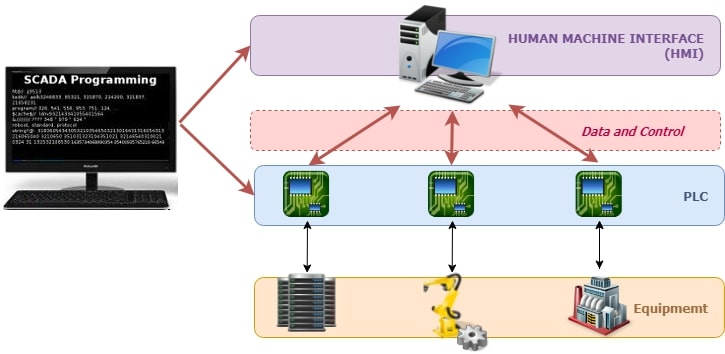
\includegraphics[width=0.7\linewidth]{Immagini/SCADA_system.jpg}
    \caption{Esempio sistema SCADA con componenti principali. Fonte: \cite{exonsys_scada}}
    \label{fig:SCADA_system.jpg}
\end{figure}

\section{Funzioni principali dello SCADA}
Un sistema SCADA svolge diverse funzioni chiave per assicurare una gestione efficace e sicura dei processi industriali, che differiscono da impianto ad impianto. Le fasi principali che generalmente uno SCADA dovrebbe fornire sono:
\begin{itemize}
    \item Acquisizione e raccolta dati: i sistemi SCADA acquisiscono dati dai dispositivi correlati di metadati e li trasferiscono al sistema centrale. Questo avviene in tempo reale per fornire continuamente consistenza sui vari parametri di processo.
    \item Visualizzazione e monitoraggio dei dati in tempo reale: i dati raccolti vengono rappresentati grazie all'HMI in formati intuitivi per favorire la lettura da parte degli operatori, attraverso grafici, tabelle interattive, led per allarmi e diagrammi di flusso.
    \item Archiviazione e storicizzazione del dato: vengono registrati i dati storici sia per analisi successive, sia per tenere traccia delle performance dell'impianto. Risultano essenziali per ottimizzare processi e per la manutenzione predittiva; inoltre i dati possono essere salvati su archivi locali o database relazionali, così da poter essere usufruibili sia tramite i formati sopra citati oppure esportati direttamente su sistemi esterni.
    \item Gestione eventi: un sistema SCADA genera allarmi e warning per segnalare criticità/anomalie nei parametri monitorati, sono una delle funzionalità cardine degli SCADA e richiedono sempre l'interazione con un operatore per evitare guasti o problemi di sicurezza. Inoltre tutti gli eventi vengono registrati e documentati per eventuali verifiche future.
    \item Controllo e manutenzione manuale: i sistemi SCADA oltre che a interfacciarsi con gli operatori, si interfacciano anche con l'impianto. Tale funzionalità è sempre più utilizzata e richiesta dai clienti per i sistemi SCADA, favorendo più flessibilità al sistema stesso, ma anche più complessità a livello progettuale.
\end{itemize}
\begin{figure}
    \centering
    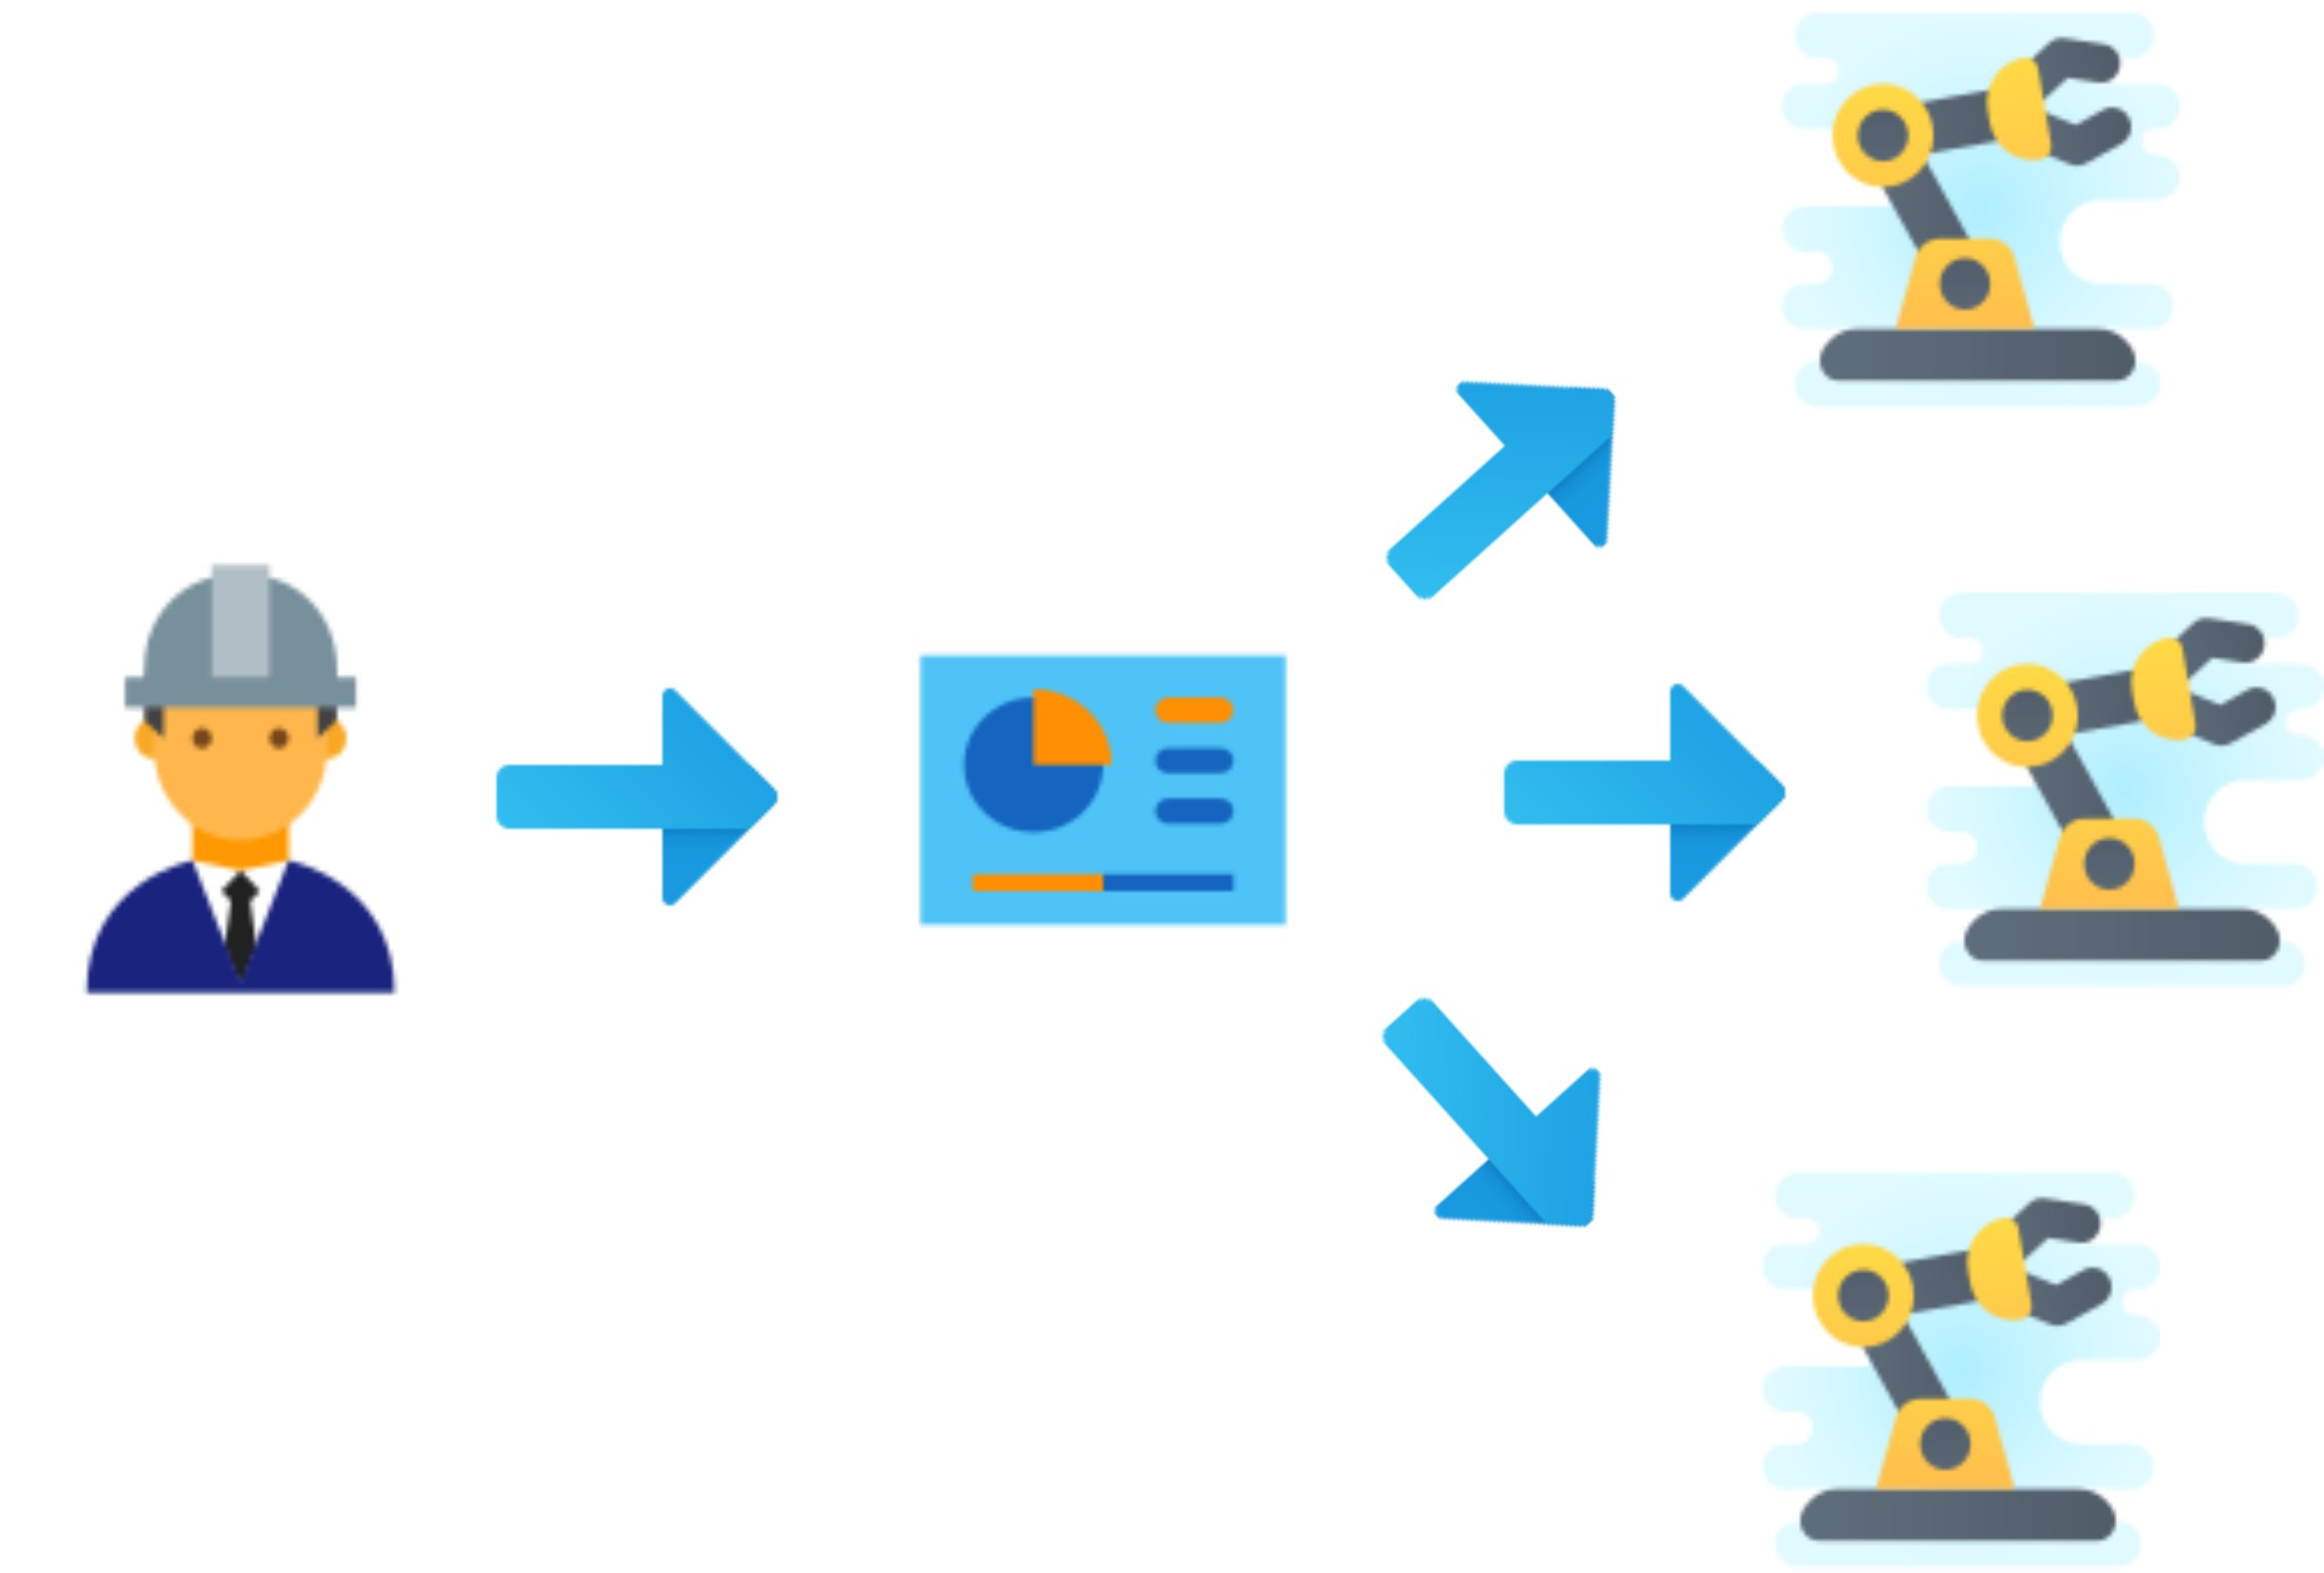
\includegraphics[width=0.5\linewidth]{Immagini/Operatore_SCADA.jpg}
    \caption{Gestione impianto tramite SCADA}
    \label{fig:Operatore_SCADA.jpg}
\end{figure}

\section{Piattaforma SCADA e Strumenti Software per la progettazione}
Con il termine piattaforma SCADA indichiamo solo lo strato software che svolge il lavoro definito in precedenza. Esistono diverse piattaforme che permettono di progettare un'interfaccia HMI per uno SCADA, e ognuna è affiancata dai propri linguaggi di programmazione proprietari, oppure i più famosi per poter progettare interfacce più avanzate (es: Jython, VBScript, C\#, ...)

\begin{figure} [ht]
    \centering
    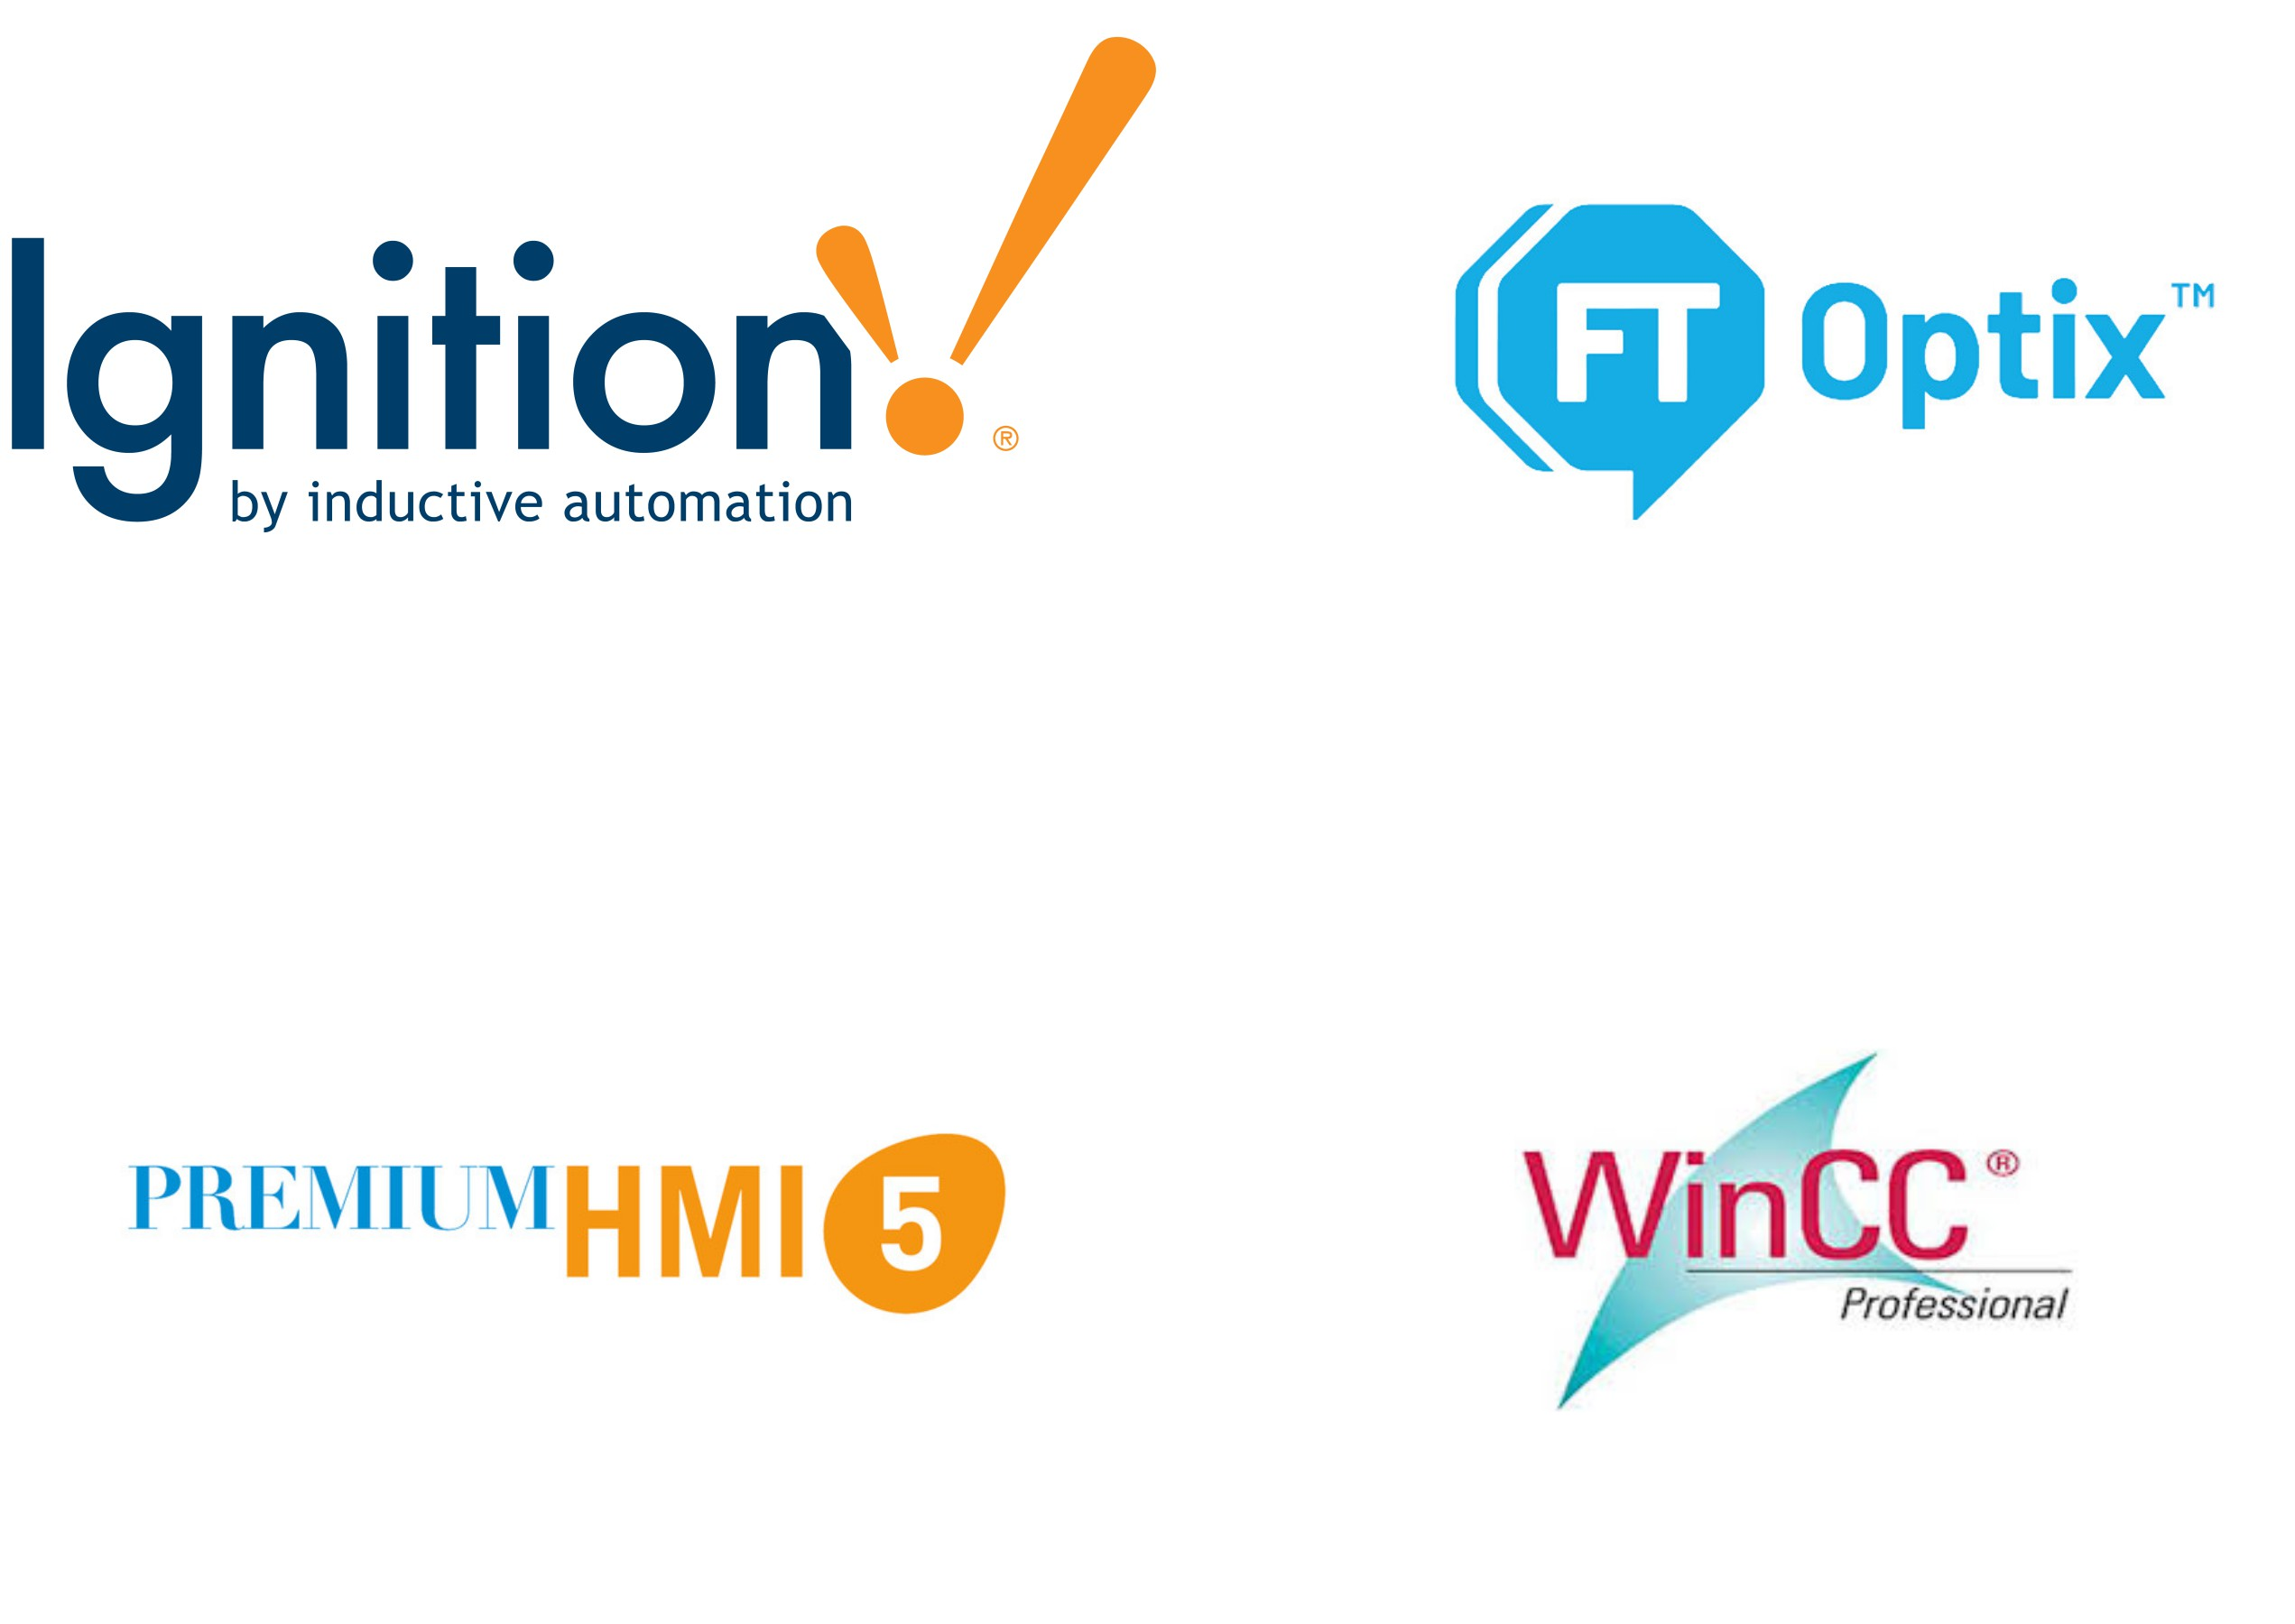
\includegraphics[width=0.5\linewidth]{Immagini/loghi.jpg}
    \caption{Esempi software per progettazione HMI}
    \label{fig:loghi.jpg}
\end{figure}

Ognuna di queste piattaforme possiede logiche diverse per poter progettare uno SCADA, nel mio caso è stata scelta come piattaforma FactoryTalk® Optix™, neo-piattaforma sviluppata da ASEM by Rockwell-Automation: 

\begin{displayquote}
    \textit{È l’innovativa piattaforma software perfetta per realizzare HMI moderne e responsive, con un’esperienza utente di alto livello, Gateway IIoT, applicazioni Edge Computing e in generale soluzioni legate alle esigenze dell’Industry 4.0.} \\ \textit{Grazie ad un’architettura completamente modulare ed estremamente flessibile sviluppata con tecnologie cross-platform, FT Optix™ permette di realizzare applicazioni compatibili con piattaforme ARM e x86 con sistemi operativi Windows e Linux, garantendo la massima flessibilità ai progettisti, che possono scegliere la piattaforma che meglio si adatta all’applicazione.} \\ \textit{FT Optix™ fa parte della suite cloud-based FactoryTalk® Design Hub™, che permette al team di progettazione di collaborare allo sviluppo dell’applicazione HMI tramite un sistema di controllo di versione distribuito, semplificando la gestione del software, aumentando la produttività ed accelerando il time to market.}\textsuperscript{\cite{asemautomation}}
\end{displayquote}

La scelta di approcciare a questa piattaforma di sviluppo è nata dal fatto che in REA l'innovazione è alla base della politica aziendale e il passaggio ad un nuovo software rappresenta la scelta perfetta per rimanere al passo con i tempi. Il software possiede un'interfaccia simile alle altre controparti ma con l'aggiunta che per SCADA più avanzati è possibile sfruttare l'uso di C\# in ambienti di sviluppo basati su .NET. Oltre a questo ho dovuto interfacciarmi con diversi software e librerie per poter far funzionare lo SCADA. 
Sul fronte C\# e ambiente di sviluppo, la scelta è ricaduta su Visual Studio Community per l'ampia customizzazione e il supporto continuo da parte di Microsoft. Inoltre per quanto riguarda la gestione di tutti i dati interni allo SCADA, due sono state le scelte su cui lavorare:
\begin{enumerate}
    \item Database locale di Optix™: per creare e gestire il database in SQLite e con l'ausilio di DB4S, è stato possibile interfacciarsi anche con le macchine più datate.
    \item Microsoft SQL Server Management Studio (SSMS): applicativo utilizzato già in REA per gestire vari database lato Server per gli impianti più complessi.
\end{enumerate}
Infine per il controllo delle versioni del progetto, data l'integrazione tra FT Optix™ e Git, la scelta è ricaduta su Git per tenere traccia di tutte le varie versioni dello SCADA durante lo sviluppo, eventualmente collaborare con altri sviluppatori e mantenere uno storico delle revisioni. 

\subsection{Lista Software utilizzati}
Ecco la lista dei software utilizzati durante la progettazione del sistema SCADA durante il tirocinio:
\begin{itemize}
    \item \textbf{FT Optix™}: versione 1.4.2.3
    \item \textbf{Microsoft Visual Studio 2022}: versione 17.11
    \item \textbf{Microsoft SQL Server Management Studio (SSMS)}: versione 20
    \item \textbf{DB Browser for SQLite (DB4S)}: versione 3.13.0
    \item \textbf{Git}: versione 2.47.0, direttamente da \textbf{GitHub Desktop}
\end{itemize}

\subsection{Struttura Generale di FactoryTalk Optix™}
FT Optix™ è un software strutturato per fornire modularità ai componenti utilizzati affinché i progetti possano essere suddivisi in componenti riutilizzabili, ciascuno con logica indipendente, e che possono essere richiamati in più parti dell'applicazione. Inoltre, come già anticipato, permette la gestione dei progetti multi-utente: con supporto per lo sviluppo collaborativo grazie al versionamento e controllo delle modifiche, oltre al supporto per protocolli industriali, come OPC UA, Modbus TCP/RTU, Ethernet/IP e altri standard di automazione. Altra caratteristica del software è la struttura a incapsulamento dei sinottici: come nella programmazione ad oggetti, viene sfruttato un tipo di design gerarchico, dove sono presenti oggetti grafici compositi, definiti Sinottici. Questi includono componenti nidificate con proprietà specifiche, logiche ed eventi. Inoltre, è possibile creare dei template parametrizzati per simulare macchinari, sensori o attuatori. Tutti questi oggetti grafici possono essere salvati in librerie condivise e riutilizzati in progetti diversi, riducendo tempi di sviluppo e migliorando la consistenza, oltre al fatto che è possibile utilizzare controlli avanzati come grafici, griglie e dashboard dinamiche per avere maggior controllo durante la progettazione. Infine, è possibile sfruttare sinottici reattivi - permettendo l'adattamento a diverse risoluzioni e formati dei pannelli HMI - e associare eventi o trigger ad ogni oggetto per eseguire azioni come aggiornamenti in tempo reale, invio di allarmi o gestione degli errori. Dal lato usabilità, fornisce simulazione attraverso ambiente di sviluppo, ossia è in grado di simulare il progetto completo con dati fittizi prima della messa in servizio, oltre a strumenti integrati per il debugging e la risoluzione di problemi, con visualizzazione di log e delle variabili in tempo reale.

\begin{figure} [ht]
    \centering
    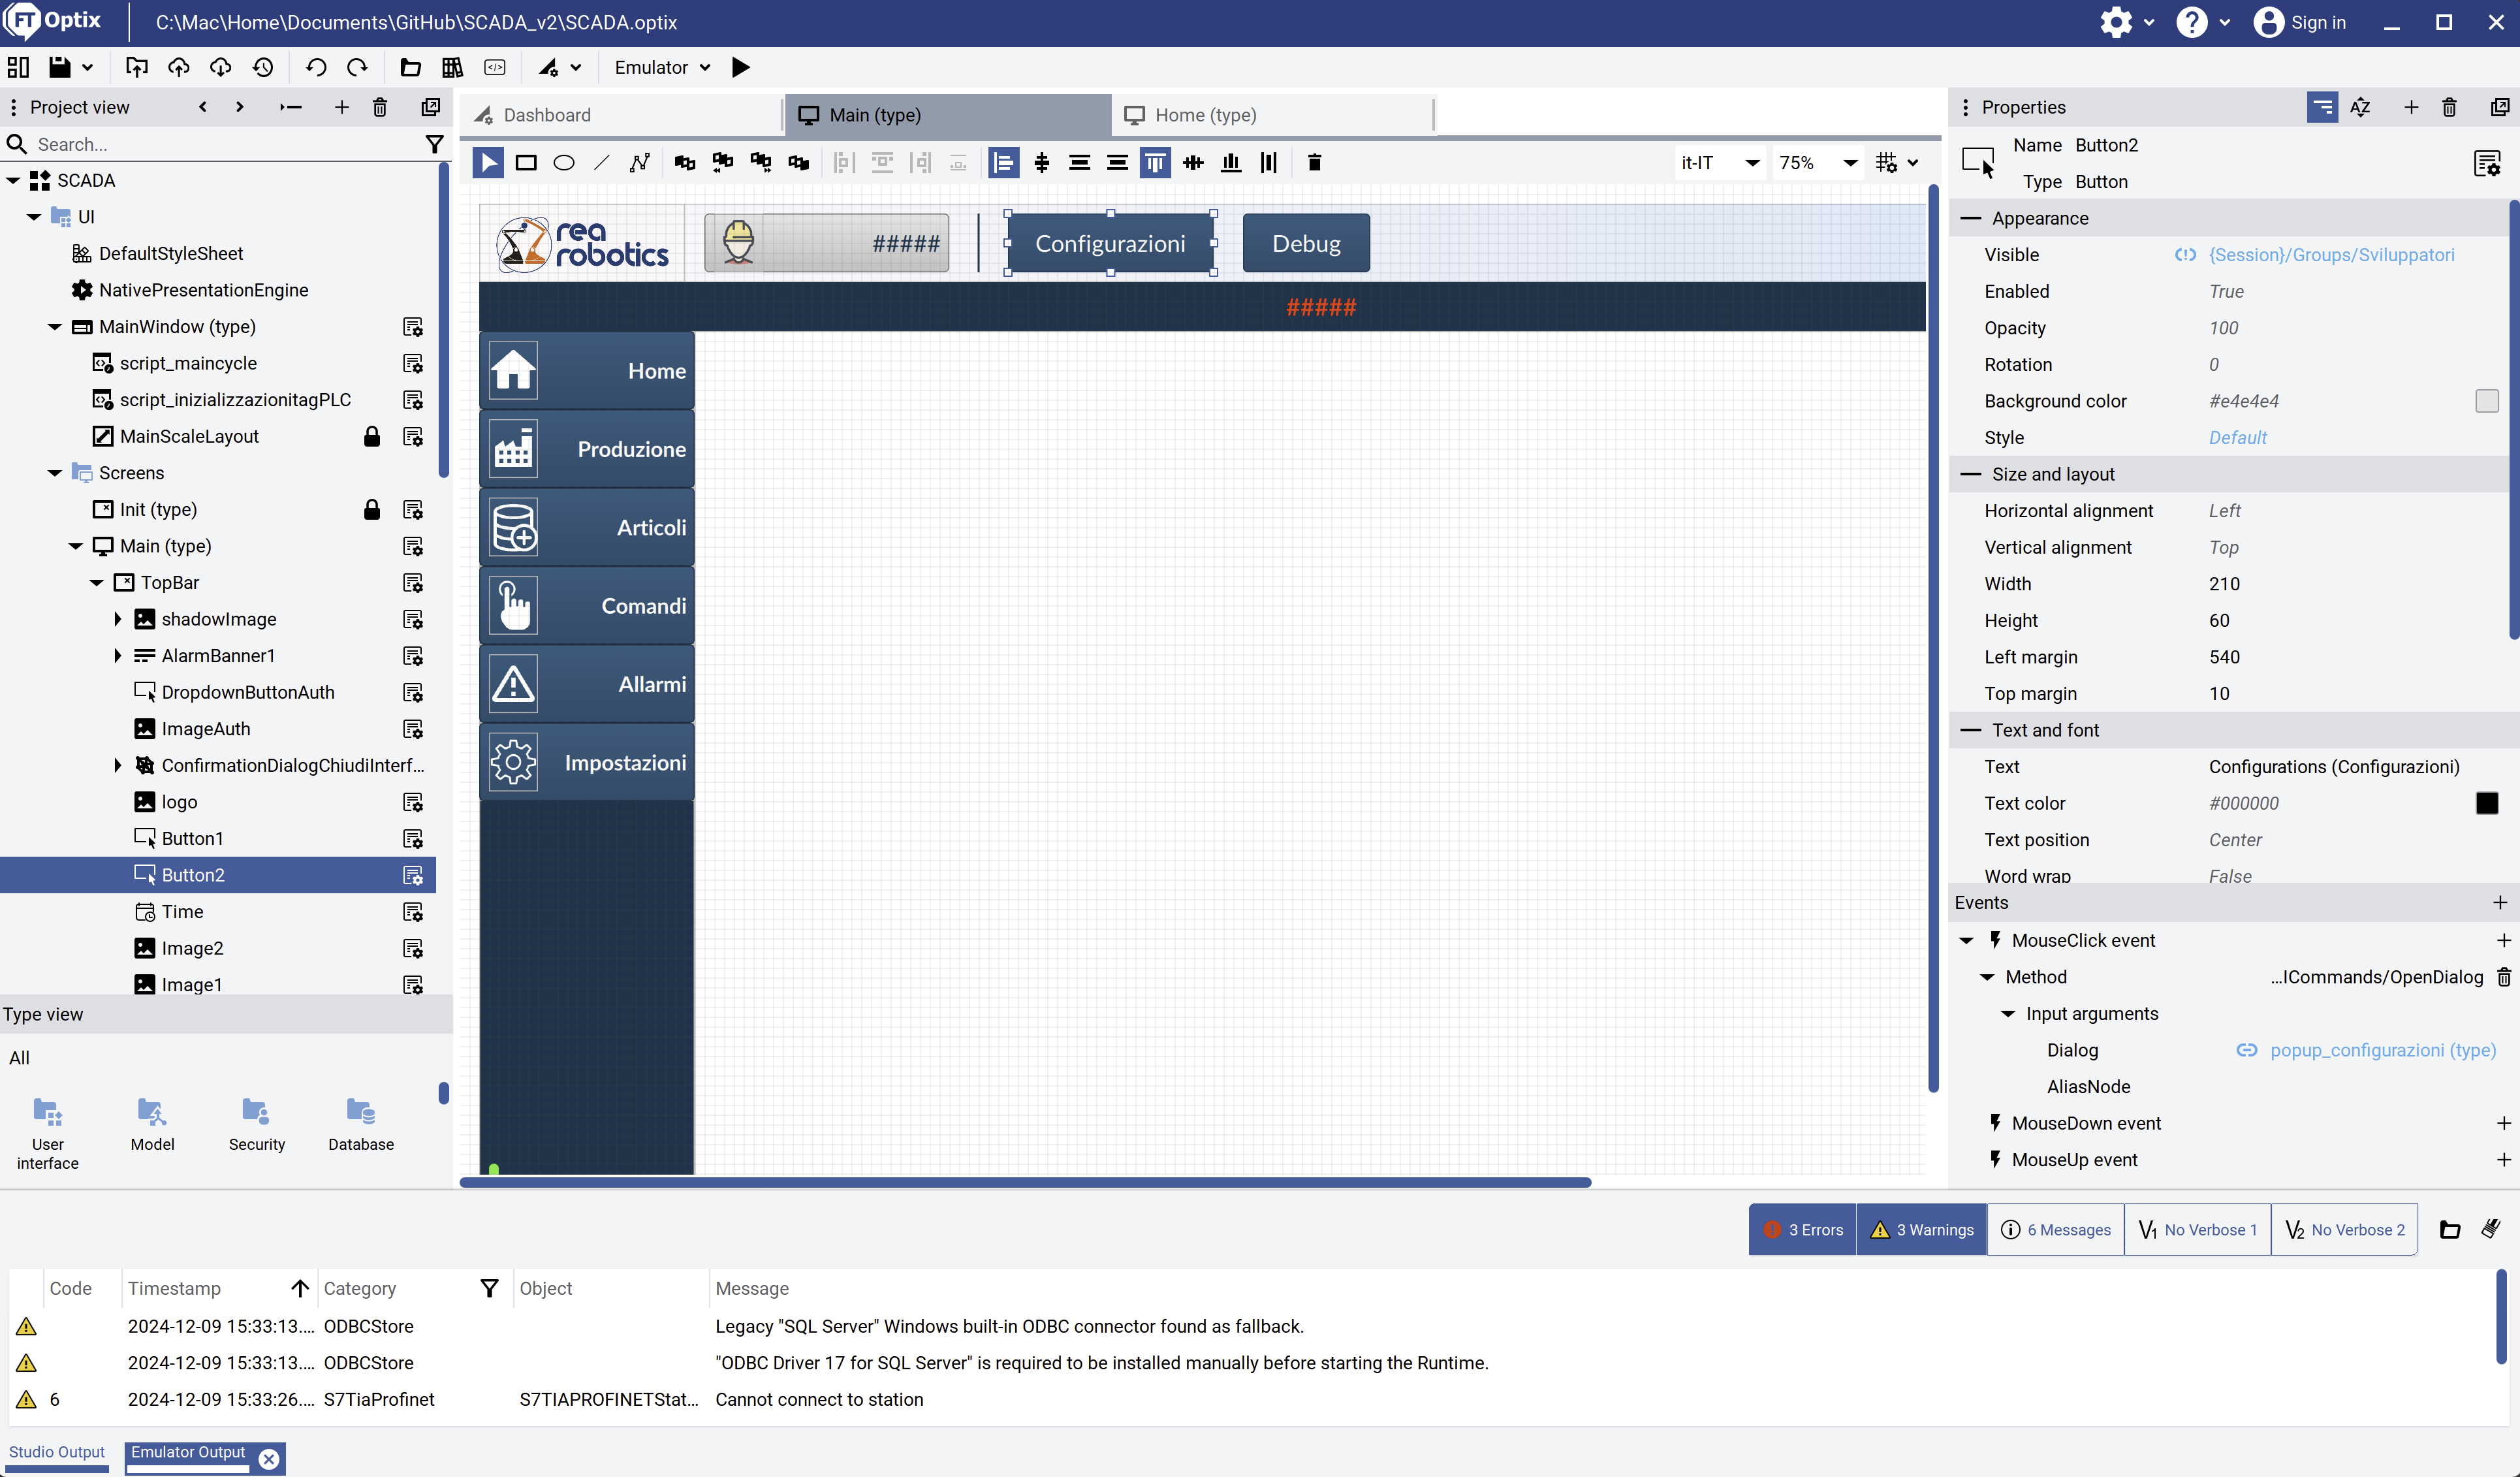
\includegraphics[width=0.5\linewidth]{Immagini/dashboard.png}
    \caption{Illustrazione dashboard di progetto}
    \label{fig:dashboard.png}
\end{figure}
    \chapter{Progettazione del sistema SCADA}

La progettazione di un sistema SCADA è un processo articolato e strategico, che richiede attenta pianificazione e un ampio impiego di risorse. Senza una struttura ben definita, infatti, si possono generare configurazioni di prodotto che necessitano di essere successivamente ripensate, portando inevitabilmente a un incremento di costi, non solo in termini di tempo, ma anche di risorse umane.
Per garantire un corretto avanzamento e rispondere in modo efficiente alle aspettative del cliente, è buona norma suddividere il lavoro in fasi predeterminate. In tal modo, si può procedere con maggiore chiarezza, sapendo già dal principio quali aspetti richiederanno attenzione specifica nelle varie fasi del progetto. Nel mio caso, il lavoro è stato suddiviso in quattro fasi principali:
\begin{enumerate}
    \item Analisi dei requisiti
    \item Strutturazione dell'HMI
    \item Gestione Database
    \item Sviluppo back-end con integrazione al PLC
\end{enumerate}
Ognuna di queste fasi ha contribuito in modo sostanziale a preservare la coerenza e l'integrità del prodotto finito, consentendo di ottenere un risultato che rispecchiasse fedelmente le richieste.

\section{Analisi dei requisiti del cliente}

La prima fase - definita anche come fase di design - prevede un momento di dialogo approfondito con il cliente per comprendere e prendere nota di tutte le necessità, in modo da tradurle in specifiche dettagliate, misurabili e quindi concretamente realizzabili dal team. L'analisi dei requisiti prevede diverse attività, la cui applicazione varia in base alla natura del prodotto finale. Oltre alla raccolta, è fondamentale l'organizzazione del loro sviluppo, soprattutto nei progetti più complessi in cui è necessario stratificare il lavoro tra più individui. 

Per quanto riguarda il mio progetto, dato l'obiettivo di creare un sistema che potesse essere altamente modulare e in grado di costituire una base solida per futuri progetti, mi è stato richiesto di soffermarmi su alcuni aspetti di fondamentale rilevanza:
\begin{enumerate}
    \item Creare un'interfaccia quanto più user-friendly possibile, per facilitare l'utilizzo e l'accessibilità da parte degli operatori di macchina.
    \item Definire un "ricettario" di base, ovvero una struttura configurabile e facilmente aggiornabile, sotto il nome di "anagrafica articoli".
    \item Definire una sezione dedicata agli ordini di produzione che includa sia i comandi di produzione per la gestione operativa, sia gli storici. 
    \item Implementare un sistema efficiente per la gestione e l'accesso agli allarmi e warning, essenziale per il monitoraggio e la diagnostica.
    \item Creare scorciatoie che permettono allo sviluppatore di poter testare il prodotto sia in fase di sviluppo, che a prodotto finito, anche tramite tele-assistenza.
\end{enumerate}

\section{Strutturazione HMI (Human Machine Interface)}
Per la realizzazione dell'HMI, l'azienda mi ha mostrato altri prodotti fornendomi le basi per comprendere il funzionamento delle interfacce. Dopo aver ricevuto piena autonomia decisionale da parte dell'azienda, ho sviluppato un approccio originale, scegliendo di procedere nel seguente modo. All'interno di FT Optix™, per prima cosa l'interfaccia è stata organizzata in una finestra principale denominata \textit{MainWindow}\textsuperscript{\cite{rockwelloptixmainwindow}} (Figura \ref{fig:HMI00.png}), a sua volta suddivisa in 3 sotto-pannelli:
\begin{itemize}
    \item Pannello di stato
    \item Pannello di funzione
    \item Pannello di menù
\end{itemize}
Il \textbf{Pannello di stato} è un elemento presente in tutta l'interfaccia e di conseguenza visibile in ogni menù e sotto-menù. La sua presenza è fondamentale poiché contiene al suo interno informazioni per il funzionamento dell'interfaccia stessa. Procedendo da sinistra troviamo il logo dell'azienda produttrice dell'impianto, che in questo caso è Rea Robotics, per dare riconoscibilità e identità a tutto il sistema. Subito dopo è presente un indicatore che contiene il nome dell'operatore che sta utilizzando la macchina (di default impostato ad anonimo). Se viene selezionato, apre un menù a tendina da cui è possibile poter eseguire l'accesso, sia come operatore, sia come sviluppatore. Tale distinzione è importante perché alcune funzioni dell'interfaccia sono accessibili solo a figure autorizzate come gli sviluppatori, per garantire sicurezza e integrità delle operazioni. 
Continuando verso destra è presente l'orario, utile per avere sempre sotto controllo il tempo durante le operazioni, e il pulsante per la selezione della lingua, che mostra l'icona della lingua attualmente attiva: l'interfaccia è stata progettata per poter funzionare sia in lingua italiana sia in lingua inglese, garantendo maggiore adattabilità anche in ambienti internazionali. Infine è presente il pulsante di spegnimento, che permette di chiudere l'interfaccia in modo sicuro. Per prevenire chiusure accidentali, alla pressione appare un popup che richiede un'ulteriore conferma di spegnimento della macchina, evitando che un tocco involontario possa interrompere il lavoro dell'operatore.
Nella parte inferiore di questo pannello è presente una sezione blu che si occupa di monitorare lo stato degli allarmi e avvisi. In caso di problemi, tale sezione mostra chiaramente l'allarme e la descrizione rilevata, assicurando così pronta visibilità delle condizioni operative del sistema.

\begin{figure} 
    \centering
    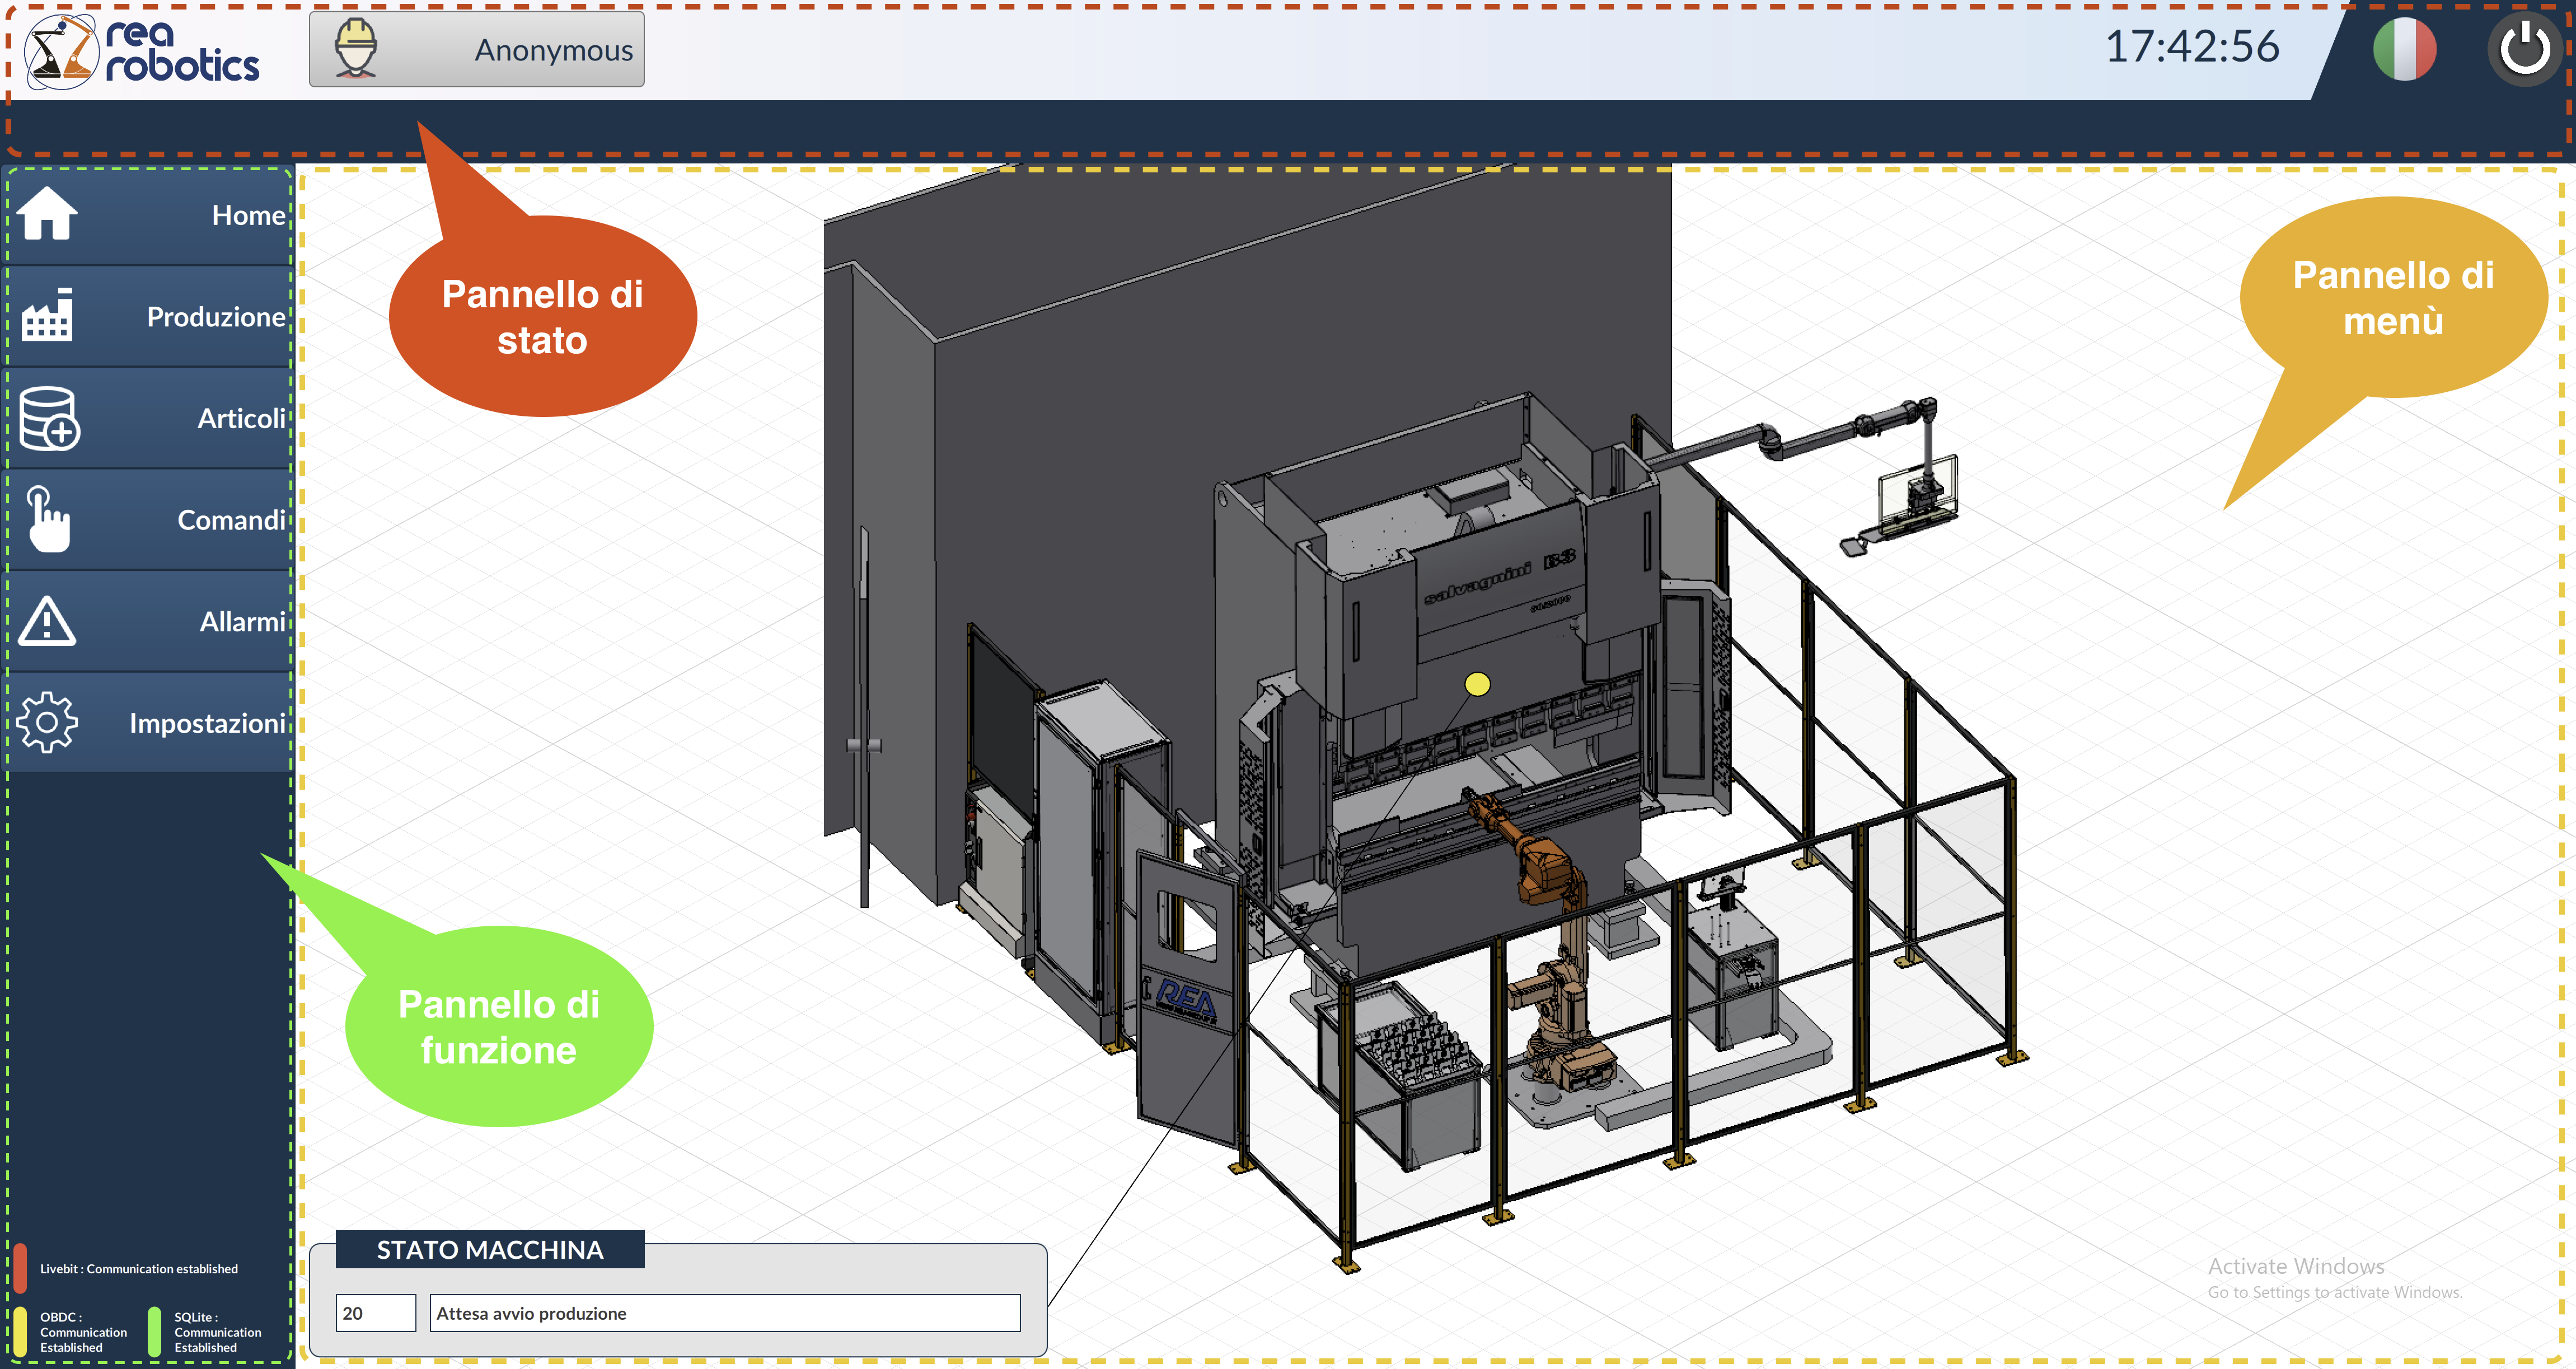
\includegraphics[width=1\linewidth]{Immagini/HMI00.png}
    \caption{Suddivisione interfaccia HMI}
    \label{fig:HMI00.png}
\end{figure}

Il \textbf{Pannello di funzione}, come il pannello di stato, è un elemento fisso che permette la navigazione attraverso i vari menù. Questo pannello è costituito da un layout verticale con una serie di pulsanti che consentono all'operatore di accedere a tutte le principali sezioni dell'interfaccia. Ogni pulsante identifica un menù specifico e, una volta selezionato, consente di passare rapidamente alla schermata desiderata, interagendo dinamicamente con il pannello di menù posizionato alla sua destra.
Il primo bottone è denominato \textit{Home} e offre una panoramica generale dello stato della macchina. In macchine più complesse permette anche la visualizzazione di indicatori di stato delle componenti. Il secondo invece permette di accedere alla \textit{Produzione}, dove l'operatore può decidere di azionare la produzione. Il terzo bottone apre la sezione \textit{Anagrafica articoli}, in cui è possibile inserire e visualizzare tutti i parametri di riferimento degli articoli dell'impianto. A seguire, troviamo la sezione \textit{Comandi manuali}, dove è possibile impartire comandi specifici direttamente al robot di lavoro. Ancora più in basso, sono presenti i bottoni della sezione: \textit{Allarmi} che forniscono una panoramica dettagliata di tutti gli allarmi e avvisi attivi. Infine, \textit{Impostazioni} dove sono presenti i vari settaggi relativi sia allo SCADA sia ai parametri della macchina. 
Nella parte inferiore del pannello di funzione sono presenti tre LED, ognuno dei quali svolge una funzione di monitoraggio importante. Il primo LED, partendo dall'alto, segnala lo stato di collegamento con la Macchina a stati, permettendo di verificare se il programma dello SCADA funziona correttamente. Il secondo e il terzo LED, invece, mostrano rispettivamente lo stato di collegamento con l'ODBC, ovvero il server su cui gira il database, e lo stato di collegamento al database locale in SQLite, che assicurano che l'interfaccia sia connessa correttamente alle risorse necessarie per il suo funzionamento.

Per ultimo abbiamo il \textbf{Pannello di menù}, che a differenza degli altri due, è interamente dinamico. Questo pannello occupa circa l'80\% di tutta l'interfaccia e ha il compito di visualizzare le varie schermate dei menù selezionate tramite il pannello di funzione. 

\begin{figure} [!ht]
    \centering
    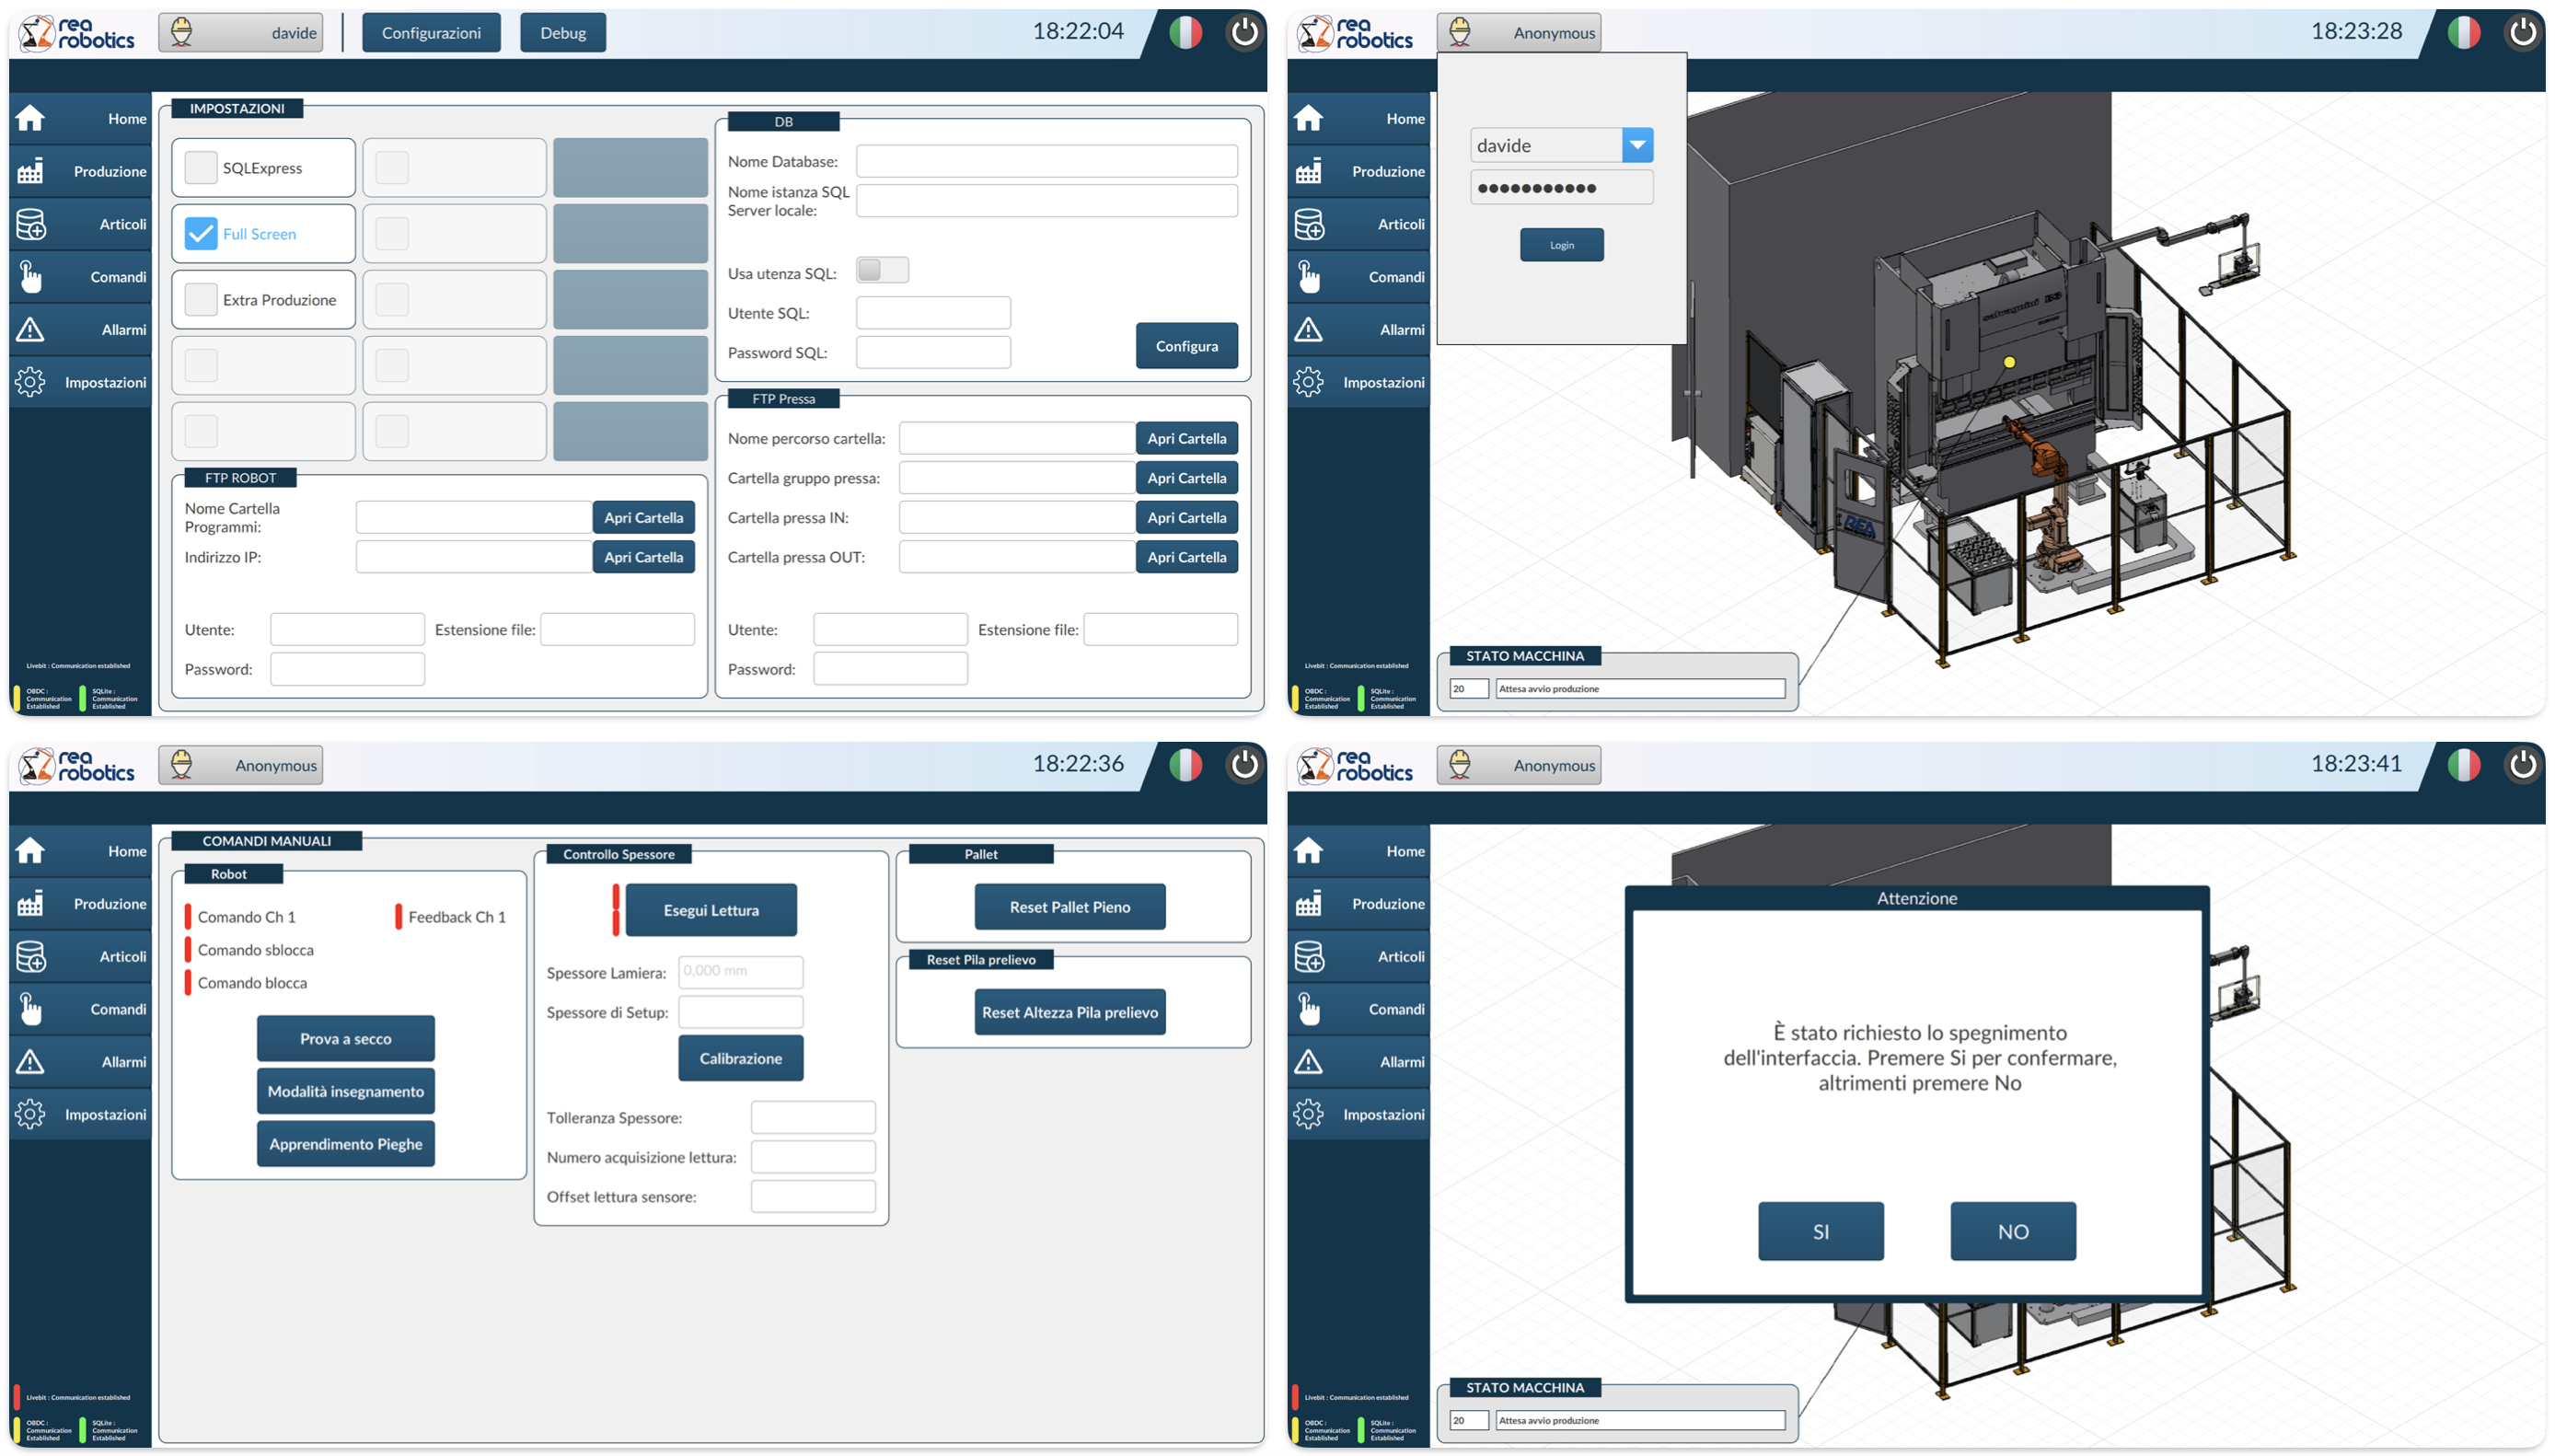
\includegraphics[width=1\linewidth]{Immagini/HMI01.png}
    \caption{4 illustrazioni dell'HMI}
    \label{fig:HMI01.png}
\end{figure}

\subsection{Considerazioni tecniche sulla risoluzione}
Grazie alla tecnologia responsive presente nativamente su FT Optix™, l'intero HMI è adattabile e scalabile su qualsiasi display, garantendo una corretta visualizzazione indipendentemente dalle dimensioni dello schermo. Tuttavia, poiché nel nostro caso lo SCADA è progettato per essere utilizzato principalmente su pannelli con risoluzione Full HD (1920x1080), è di fondamentale importanza che tutta l'interfaccia sia leggibile e fruibile dall'operatore senza barre di scorrimento laterali.
Considerando a maggior ragione che lo SCADA sarà utilizzato su dispositivi dotati di tecnologia touch in ambienti industriali, è cruciale che ogni elemento risulti chiaro, affidabile e di facile accesso. La leggibilità e la precisione dei comandi sono fondamentali per garantire la sicurezza e l'efficacia delle operazioni svolte dall'operatore in tali contesti.

\section{Gestione Database per la produzione}

Per quanto riguarda il database ho deciso di adottare diverse metodologie per la gestione dati. La prima esigenza dell'azienda è stata creare un ricettario per mantenere una serie di record con attributi ben specifici, e che permettesse l'integrazione e la comunicazione verso la scheda di produzione. La mia proposta di soluzione ideale è stata quella di suddividere il database in due tabelle: una completamente dedicata alla parte di \textit{Anagrafica articoli} presenti in macchina, e l'altra che riguardasse la \textit{Produzione}, in cui vengono registrati gli ordini. Questa rappresenta solo la prima fase di progettazione, poiché nello SCADA è necessario anche avere accesso ad altri dati, tra cui: lo \textit{Storico Produzioni}, che archivia tutte le produzioni completate, sia con esito positivo che negativo; tutte le variabili che potrebbero influire sull'integrità dello stato di un ordine (ad es: l'extra produzione); e tutti gli interventi effettuati tramite input all'HMI, come l'importazione e l'esportazione delle ricette. Infine, ho deciso di integrare all'HMI non solo il database locale creato da me, ma anche il SSMS fornito dall'azienda, per garantire maggiore flessibilità al sistema.

\subsection{Anagrafica Articoli} 
Questa sezione si occupa della gestione dell'inserimento di nuovi articoli da produrre nell'impianto. La progettazione ha richiesto due tipi di interventi: il primo ha riguardato la gestione del front-end dell'anagrafica; il secondo ha coinvolto la parte di back-end, con particolare attenzione a bottoni e gestione database. 

Il lavoro è iniziato con la creazione del menù, in particolare di un'interfaccia dedicata che possa integrare tutti i comandi necessari. Grazie a FT Optix™, è possibile implementare una sezione di inserimento dei singoli articoli composta dagli attributi richiesti dal sistema. In aggiunta, è stata predisposta una sezione di visualizzazione, che mostra tutti i dati del database, compresi gli attributi richiesti in precedenza. Per facilitare la gestione dei dati, è stato sfruttato un oggetto di tipo \textit{DataGridView}\textsuperscript{\cite{factorytalk_datagrid_example}}, che emula il funzionamento di una tabella, rendendo chiara e accessibile la consultazione dei dati. Dato che uno SCADA industriale deve gestire qualche centinaio di articoli, sono stati implementati sia un sistema di filtraggio dei prodotti in base a parametri specifici (selezionando gli attributi d'interesse), sia una barra di ricerca che permette di individuare rapidamente un prodotto già presente nel sistema. Inoltre, su richiesta, è stata aggiunta una sezione in basso (Figura: \ref{fig:AnagraficaArticoli.png}) per l'esportazione e l'importazione delle ricette, consentendo al sistema di caricare serie di articoli preconfigurati dal cliente, velocizzando e semplificando il processo di inserimento articoli.

\begin{figure} 
    \centering
    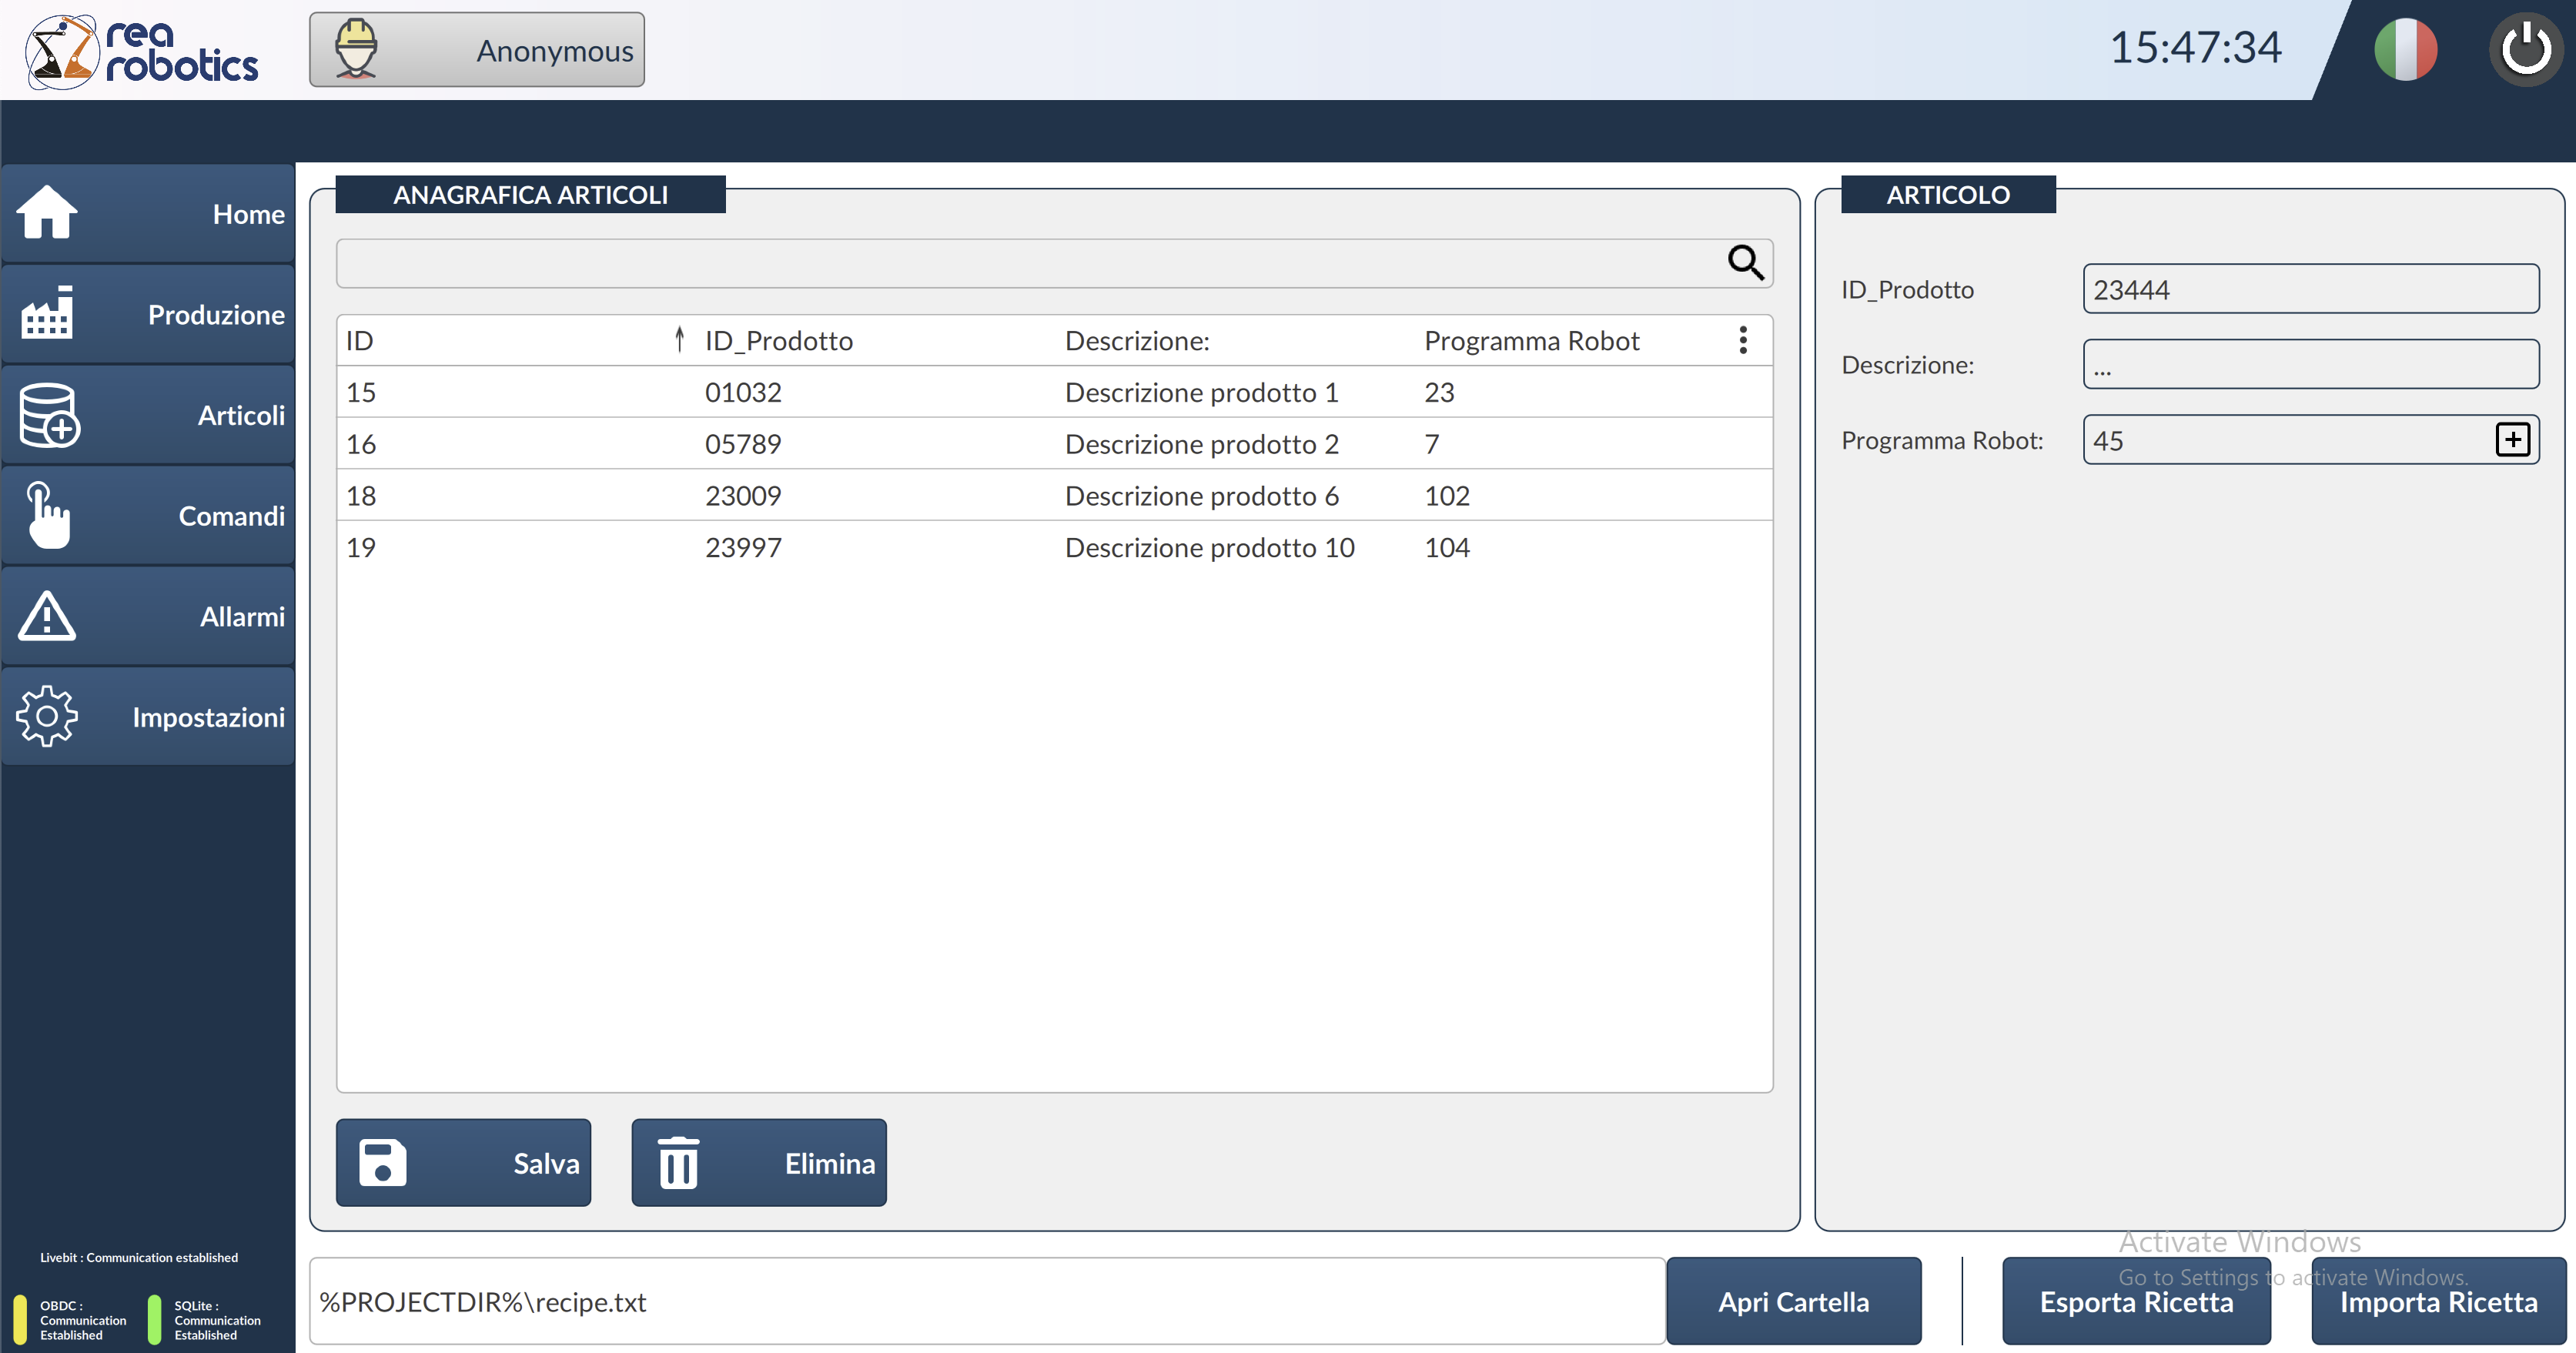
\includegraphics[width=1\linewidth]{Immagini/AnagraficaArticoli.png}
    \caption{Illustrazioni sezione \textit{Articoli}}
    \label{fig:AnagraficaArticoli.png}
\end{figure}

Per quanto riguarda la parte di back-end, il primo passo consiste nel configurare il database di riferimento. All'interno della Project View nella cartella DataStores deve essere creato un oggetto di tipo \textit{Embedded database}, che permette di importare un database \verb|.sqlite| su cui lavorare\textsuperscript{\cite{rockwelloptixdatastore}}. Successivamente, è necessario eseguire una serie di passaggi per poter impostare correttamente la struttura delle tabelle:

\begin{enumerate}
    \item Importare/impostare in \textit{Configuration} il nome del file del database da cui l'eseguibile dovrà estrarre i dati.
    \item Creare, tramite FT Optix™, le tabelle sotto il nome di \textit{RecipeSchema}, includendo tutti gli attributi di interesse necessari per la gestione delle ricette.
    \item Aprire il file creato, sotto il nome di \verb|filename.sqlite| tramite un software come DB4S, presente all'interno della cartella ApplicationFiles del programma, per impostare eventuali vincoli del database. Questo ultimo passaggio è facoltativo e può essere omesso qualora non siano richiesti vincoli specifici per i dati da raccogliere.
\end{enumerate} 

Prima di introdurre la sezione degli script in C\#, è importante chiarire due scelte di stile che ho adottato durante la progettazione del seguente database. Nel nostro caso ogni articolo deve essere caratterizzato da attributi ben definiti, che devono essere sempre presenti, indipendentemente dalla macchina su cui lo SCADA dovrà essere installato. In particolare:

\begin{itemize}
    \item \textbf{\textit{ID}}: un identificatore universale per il database, configurato come un intero, chiave primaria e auto-incrementale (\verb|INTEGER PRIMARY KEY AUTOINCREMENT|). Questo attributo permette ad ogni articolo di avere un identificativo distinto, senza mai ripetersi, nemmeno in caso di eliminazione o modifica di un prodotto. Questa scelta viene fatta per motivi di sicurezza, prevenendo eventuali conflitti di tuple in situazioni di sincronizzazione non corretta. 
    \item \textbf{\textit{Product\_ID}}: un identificatore specifico per il prodotto con vincoli meno restrittivi rispetto al primo. Questo campo non deve essere forzatamente un intero, bensì può essere anche un codice alfa-numerico, a discrezione del cliente. Come unici vincoli aggiunti, per non incorrere in errori di inserimento, ci sono l'unicità e l'obbligo di non essere nullo.
    \item \textbf{\textit{Robot\_Program}}: indica il programma che il robot dovrà utilizzare. Di norma, questi programmi sono identificati da numeri. Anche in questo caso, deve essere specificato il vincolo di obbligatorietà: non nullo, garantendo l'inserimento di un valore.
\end{itemize}
Partendo da questa base, è possibile inserire a piacimento ulteriori attributi in base alla necessità del cliente oppure dell'impianto su cui si sta lavorando, ripetendo i passaggi descritti precedentemente. 
L'altra considerazione da fare riguarda l'uso dei \textit{RecipeSchema} in FT Optix™, per cui esistono alcuni vincoli dati dal software: ad esempio, l'obbligo di anteporre il carattere \verb|/| a tutti gli attributi creati sia nel database locale sia in interfaccia. Inoltre, FT Optix™ supporta nativamente, attraverso le API, solo operazioni di base per le ricette, quali: INSERT, UPDATE, DELETE e SELECT\textsuperscript{\cite{rockwelloptixsqlquery}}. Sebbene inizialmente questo possa sembrare un vantaggio, dato che permette un accesso semplificato tramite i tool integrati, in alcuni casi può rappresentare una limitazione se si desidera interagire attraverso funzioni più complesse con il database. Per questo motivo, FT Optix™ fornisce la possibilità di creare in prima persona script in C\#, dando piena flessibilità e controllo diretto sul database al programmatore. Questa scelta si è dimostrata vincente, perchè mi ha permesso di creare script unici per la successiva gestione dei dati. 


Per quanto riguarda invece la parte di back-end, iniziamo con l'inserimento degli articoli nel database. Utilizzando i \textit{RecipeSchema}\textsuperscript{\cite{factorytalk_recipes}}, FT Optix™ mette a disposizione un oggetto \textit{RunTimeNetLogic}\textsuperscript{\cite{factorytalk_netlogic}} di tipo \textit{RecipeController}, che include già una serie di funzioni di base. Nel nostro caso, è necessario implementare all'interno del file \verb|RecipeController.cs| uno script che permetta l'inserimento di un prodotto in Anagrafica correttamente. In Visual Studio, creiamo quindi una funzione che verrà richiamata dal tasto SALVA presente nell'interfaccia. Per prima cosa, scriviamo il comando \verb|[ExportMethod]|(riga 2) che consente di rendere accessibile la funzione direttamente in FT Optix™ (questa pratica verrà ripetuta anche per futuri script). Successivamente, definiamo la funzione specificando gli attributi in input che ci interessa salvare. All'interno del codice, viene richiamato il database locale (oppure SSMS) tramite \verb|myStore| e la tabella di interesse \verb|myTable| (rispettivamente righe 8-9). Da qui possiamo utilizzare la funzione \verb|.Insert| di FT Optix™, con i valori precedentemente richiamati, per popolare il database (riga 18).
\begin{csharp}
...
    [ExportMethod]
    public void Insert_Product_in_Anagrafica(string Product_ID, string Descr, int Robot_Program)
    {
        try
        {
            // Inserimento nella tabella
            var myStore = Project.Current.Get<Store>("DataStores/EmbeddedDatabase1");
            var myTable = myStore.Tables.Get<Table>("RecipeSchema1");
            string[] columns = { "Name", "/Descr", "/Robot_Program", "/Product_ID" };
            var values = new object[1, 4];
            values[0, 0] = Product_ID;
            values[0, 1] = Descr;
            values[0, 2] = Robot_Program;
            values[0, 3] = Product_ID;
    
            // Eseguire la query di inserimento
            myTable.Insert(columns, values);
    
            // Se l'operazione è andata a buon fine
            Log.Info("RecipeSchema1", "Inserimento riuscito: " + values[0, 1]);
        }
        catch (Exception ex)
        {
            // In caso di errore, viene catturata l'eccezione e viene stampato il messaggio d'errore
            Log.Error("RecipeSchema1", "Errore durante l'inserimento: " + ex.Message);
            popup.OpenPopUp(ex.Message, 0);
        }
    }
...
\end{csharp}
Due aspetti importanti meritano attenzione in questa fase. In primo luogo, si osserva la presenza del carattere \verb|/| negli attributi, come richiesto dalle specifiche di FT Optix™ per le ricette. In secondo luogo, vi è un attributo \verb|Name|, il quale rappresenta un vincolo essenziale nella costruzione delle ricette in FT Optix™; nel nostro caso, assegniamo a tale campo un valore a scelta tra quelli disponibili. Inoltre, la funzione è stata inserita in un blocco \verb|try-catch| per garantire maggiore controllo su eventuali errori di inserimento in FT Optix™ (altra pratica ampliata anche ad altri script, come regola di buona programmazione).
Ora passiamo ad un'ulteriore richiesta che riguarda le importazioni di articoli esterni. In questo caso, è stato necessario avvalerci di un ulteriore oggetto, \textit{RunTimeNetLogic}, direttamente associato alla tabella, al fine di implementare una funzione capace di controllare un file esterno definito come \verb|dati.txt|. Di seguito è riportato il codice:
\begin{csharp}
...
    // Metodo per controllare e leggere il file
    private static void ControllaFile(Object source, ElapsedEventArgs e)
    {
        // Specifica la cartella e il nome del file
        string cartella = @"C:\Users\davide.quartucci\Desktop\InserimentoAnagraficaSuDB";
        string nomeFile = "dati.txt";
    
        // Cerca il file nella cartella specificata
        string percorsoFile = Path.Combine(cartella, nomeFile);
    
        if (File.Exists(percorsoFile))
        {
            try
            {
                // Leggi il contenuto del file
                string[] righe = File.ReadAllLines(percorsoFile);
    
                foreach (string riga in righe)
                {
                    try
                    {
                        // Dividi la riga in tre parti usando il separatore ';'
                        string[] campi = riga.Split(';');
    
                        if (campi.Length != 3)
                        {
                            throw new FormatException("La riga non contiene esattamente 3 campi.");
                        }
    
                        // Assegna i campi a variabili locali
                        string Product_ID = campi[0];
                        string Descr = campi[1];
                        int Robot_Program;
    
                        // Prova a convertire il terzo campo in un intero
                        if (!int.TryParse(campi[2], out Robot_Program))
                        {
                            throw new FormatException("Il campo Robot_Program non è un intero valido.");
                        }
    
                        //Esegue l'inserimento nel DB di una nuova anagrafica
                        var myStore = Project.Current.Get<Store>("DataStores/EmbeddedDatabase1");
                        var myTable = myStore.Tables.Get<Table>("RecipeSchema1");
                        string[] columns = { "Name", "/Descr", "/Robot_Program", "/Product_ID" };
                        var values = new object[1, 4];
                        values[0, 0] = Product_ID;
                        values[0, 1] = Descr;
                        values[0, 2] = Robot_Program;
                        values[0, 3] = Product_ID;
                        myTable.Insert(columns, values);
                    }
                    ... // Gestione eccezioni ed eliminazione file dopo la lettura
\end{csharp}
Nel codice appena illustrato viene richiamata la seguente funzione: \verb|dati.txt| situato in un percorso preimpostato (righe 6-7). La scelta di definire un percorso ben specifico è stata fatta per evitare problemi imprevisti durante l'inserimento dei dati. La funzione prosegue analizzando le righe del file, secondo le specifiche \textit{Product\_ID; Descrizione; Robot\_Program} (righe da 17 a 37). A partire da riga 42, il codice procede con l'inserimento all'interno del database di tutti i dati del file, e infine, lo elimina come richiesto. Ovviamente, questa funzione deve essere richiamata ciclicamente per garantire un aggiornamento continuo del database, facilitando così, ad esempio, la trasmissione di nuovi articoli dagli uffici di produzione direttamente alla macchina. Per automatizzare l'intero processo, nel metodo \verb|Start| (creato nativamente da FT Optix™) ho deciso di configurare un timer che ogni 10 secondi ripete l'operazione di lettura ed importazione degli articoli nell'anagrafica, assicurando aggiornamento costante e sincronizzazione dei dati:
\begin{csharp}
...
    private static Timer timer; // Timer per eseguire l'operazione ogni 10 secondi

    public override void Start()
    {
        // Insert code to be executed when the user-defined logic is started
        
        // Imposta e avvia il timer
        timer = new Timer(10000); // 10000 millisecondi = 10 secondi
        timer.Elapsed += ControllaFile; // Associa l'evento Elapsed all'handler
        timer.AutoReset = true; // Ripeti l'operazione ogni 10 secondi
        timer.Enabled = true; // Abilita il timer
    }
...
\end{csharp}
Per tutte le altre funzionalità, come l'eliminazione di articoli, ricerche ed importazioni/esportazioni da HMI, sono state sfruttate funzionalità di base già presenti nel programma. Il lavoro si è concentrato sull'ampliamento e personalizzazione di questi strumenti affinché si integrassero correttamente con il sistema.

\subsection{Ordini di Produzione}

Questa sezione si focalizza sulla fase di produzione degli articoli, con focus sull'inserimento, l'avvio e la gestione di una nuova produzione. La progettazione ha seguito il medesimo approccio adottato per la sezione dell'anagrafica. Per quanto riguarda l'interfaccia, ho preferito dividere la creazione di un nuovo ordine di produzione dalla gestione della produzione stessa, poiché nel monitoraggio è necessario tenere in primo piano molti più attributi rispetto alla sezione di anagrafica. Dal punto di vista progettuale, troviamo ancora un oggetto di tipo \textit{DataGridView}, che anche in questo caso serve per tenere sotto controllo lo stato degli ordini. Infatti, è stato anche configurato in modo che cambi colore in base allo stato dell'ordine: verde per gli articoli che sono attualmente in produzione, giallo per quelli in attesa e rosso per eventuali interruzioni impreviste. Anche in questa sezione è stato implementato un sistema di filtraggio, mentre nella parte inferiore della schermata troviamo un pannello che tiene sotto controllo lo stato/passo in cui si trova la macchina (il suo funzionamento verrà illustrato nella sezione \ref{sec:Sviluppo back-end e integrazione con il PLC}). Sempre nella parte inferiore della schermata, inoltre, sono presenti i pulsanti che permettono la gestione degli ordini di macchina. Prima di procedere alla fase implementativa, è stato progettato anche un popup per \textit{Nuova Produzione} (Figura:\ref{fig:Produzione.png}), che permette di inserire gli ordini in database. Questo popup è una finestra che richiede le specifiche di produzione, ovvero:
\begin{itemize}
    \item \textit{\textbf{Ordine di Produzione}}: identificativo dell'ordine, configurato come campo testuale.
    \item \textit{\textbf{Nome Articolo}}: mostra a schermo un menù a tendina che consente di selezionare il \textit{Product\_ID} dell'articolo già presente in database, ereditando tutte le caratteristiche definite nella sezione Anagrafica.
    \item \textit{\textbf{Quantità\_Richiesta}}: è la quantità dell'ordine da produrre inizialmente.
\end{itemize}

\begin{figure} 
    \centering
    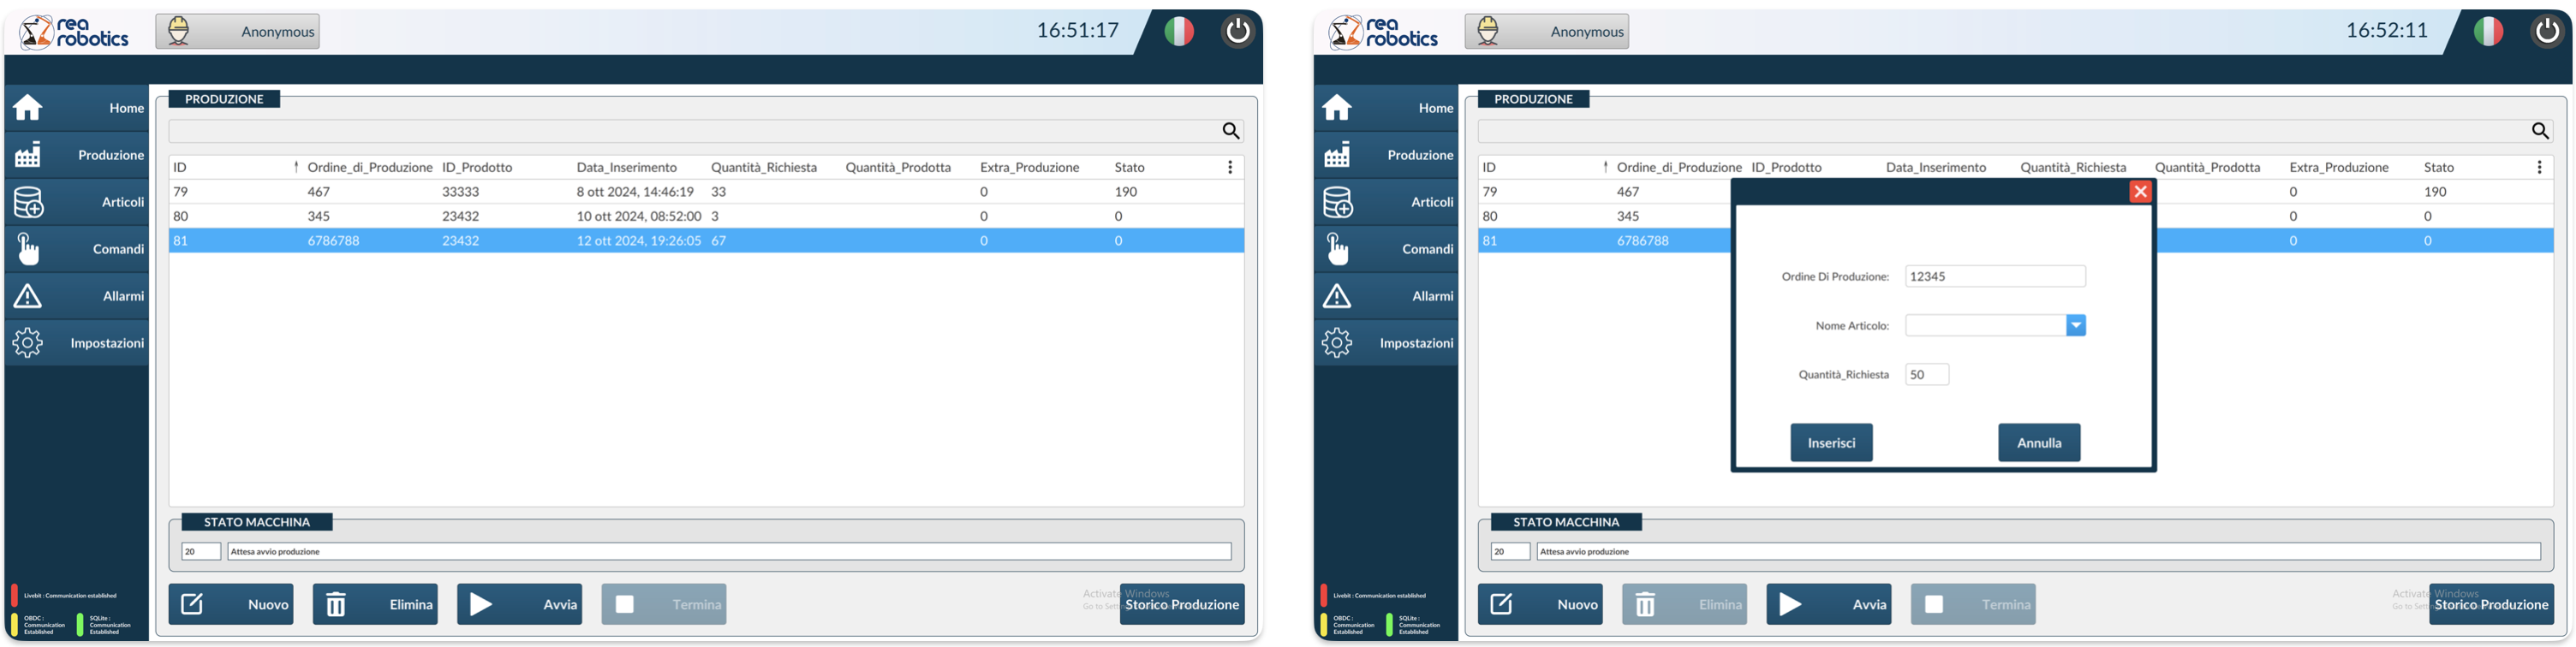
\includegraphics[width=1\linewidth]{Immagini/Produzione.png}
    \caption{Illustrazioni sezione \textit{Produzione} e sottosezione \textit{Nuova Produzione}}
    \label{fig:Produzione.png}
\end{figure}

Fatto questo, ulteriori attributi vengono impostati durante l'inserimento dell'ordine. Infatti, dopo aver specificato i dati precedenti e premuto il tasto "inserisci", viene richiamata una funzione all'interno di \verb|RecipeController.cs|, sviluppata seguendo le stesse linee guida di quella già analizzata in Anagrafica. In questo caso, poiché la produzione necessita di parametri aggiuntivi, come ad esempio: \textit{Date\_Insert, Status, Extra\_Production, ...}, questi attributi vengono inizialmente impostati su valori predefiniti. Un attributo che necessita di analisi è la Data di Inserimento (gestita a riga 16). Qui viene utilizzato \verb|DateTime.Now| per ottenere il momento esatto del salvataggio, con successivo parsing in \verb|.ToString|, come richiesto per il corretto inserimento dei dati nel database.

\begin{csharp}
...
[ExportMethod]
public void Insert_newProduction(string Odp, string NomeArticolo, int quantità)   
{
    try
    {
        // Inserimento nella tabella
        var myStore = Project.Current.Get<Store>("DataStores/EmbeddedDatabase1");
        var myTable = myStore.Tables.Get<Table>("RecipeSchema2");
        string[] columns = { "Name", "/Odp", "/NomeArticolo", "/Date_Insert", "/Quantità", "/Extra_Production", "/Total_Reject", "/Status" };
        var values = new object[1, 8];

        values[0, 0] = Odp;
        values[0, 1] = Odp;
        values[0, 2] = NomeArticolo;
        values[0, 3] = DateTime.Now.ToString("yyyy-MM-ddTHH:mm:ss.fffffffK"); 
        values[0, 4] = quantità;
        values[0, 5] = 0;
        values[0, 6] = 0;
        values[0, 7] = 0;

        // Eseguire la query di inserimento
        myTable.Insert(columns, values);

        // Se l'operazione è andata a buon fine
        Log.Info("RecipeSchema2", "Inserimento riuscito: " + values[0, 1]);
    }
    catch (Exception ex)
    {
        // In caso di errore, viene catturata l'eccezione e viene stampato il messaggio d'errore
        Log.Error("RecipeSchema2", "Errore durante l'inserimento: " + ex.Message);
        popup.OpenPopUp(ex.Message, 0);
    }
}
...
\end{csharp}

Prima di passare all'implementazione della funzione \textit{Avvia Produzione}, è necessario soffermarci su un'ulteriore richiesta da parte dell'azienda: la gestione di un'eventuale \textit{Extra Produzione} per rispondere a esigenze particolari di produzione. Per questo motivo, sono stati attuati 2 passaggi:
\begin{enumerate}
    \item Assicurarsi che l'\textit{extra produzione} sia sempre disponibile e attivabile su richiesta tramite un'opzione accessibile solamente dal programmatore.
    \item Nel caso in cui sia attiva, permettere alla macchina di poterla gestire lato back-end (che verrà approfondito nella sezione \ref{sec:Sviluppo back-end e integrazione con il PLC}).
\end{enumerate}
Per il primo punto la soluzione adottata consiste nell'inserire all'interno della sezione \textit{Impostazioni} un interruttore \textit{Extra Produzione}, attivabile esclusivamente in modalità sviluppatore o con le opportune autorizzazioni\textsuperscript{\cite{factorytalk_users_groups}}. Fatto questo è stato progettato un popup che appare al termine di ogni ciclo di produzione e, tramite un menù, chiede se si vogliono produrre ulteriori componenti, permettendo così alla macchina di riavviare il ciclo produttivo (Figura:\ref{fig:Extraproduzione.png}).

\begin{figure} 
    \centering
    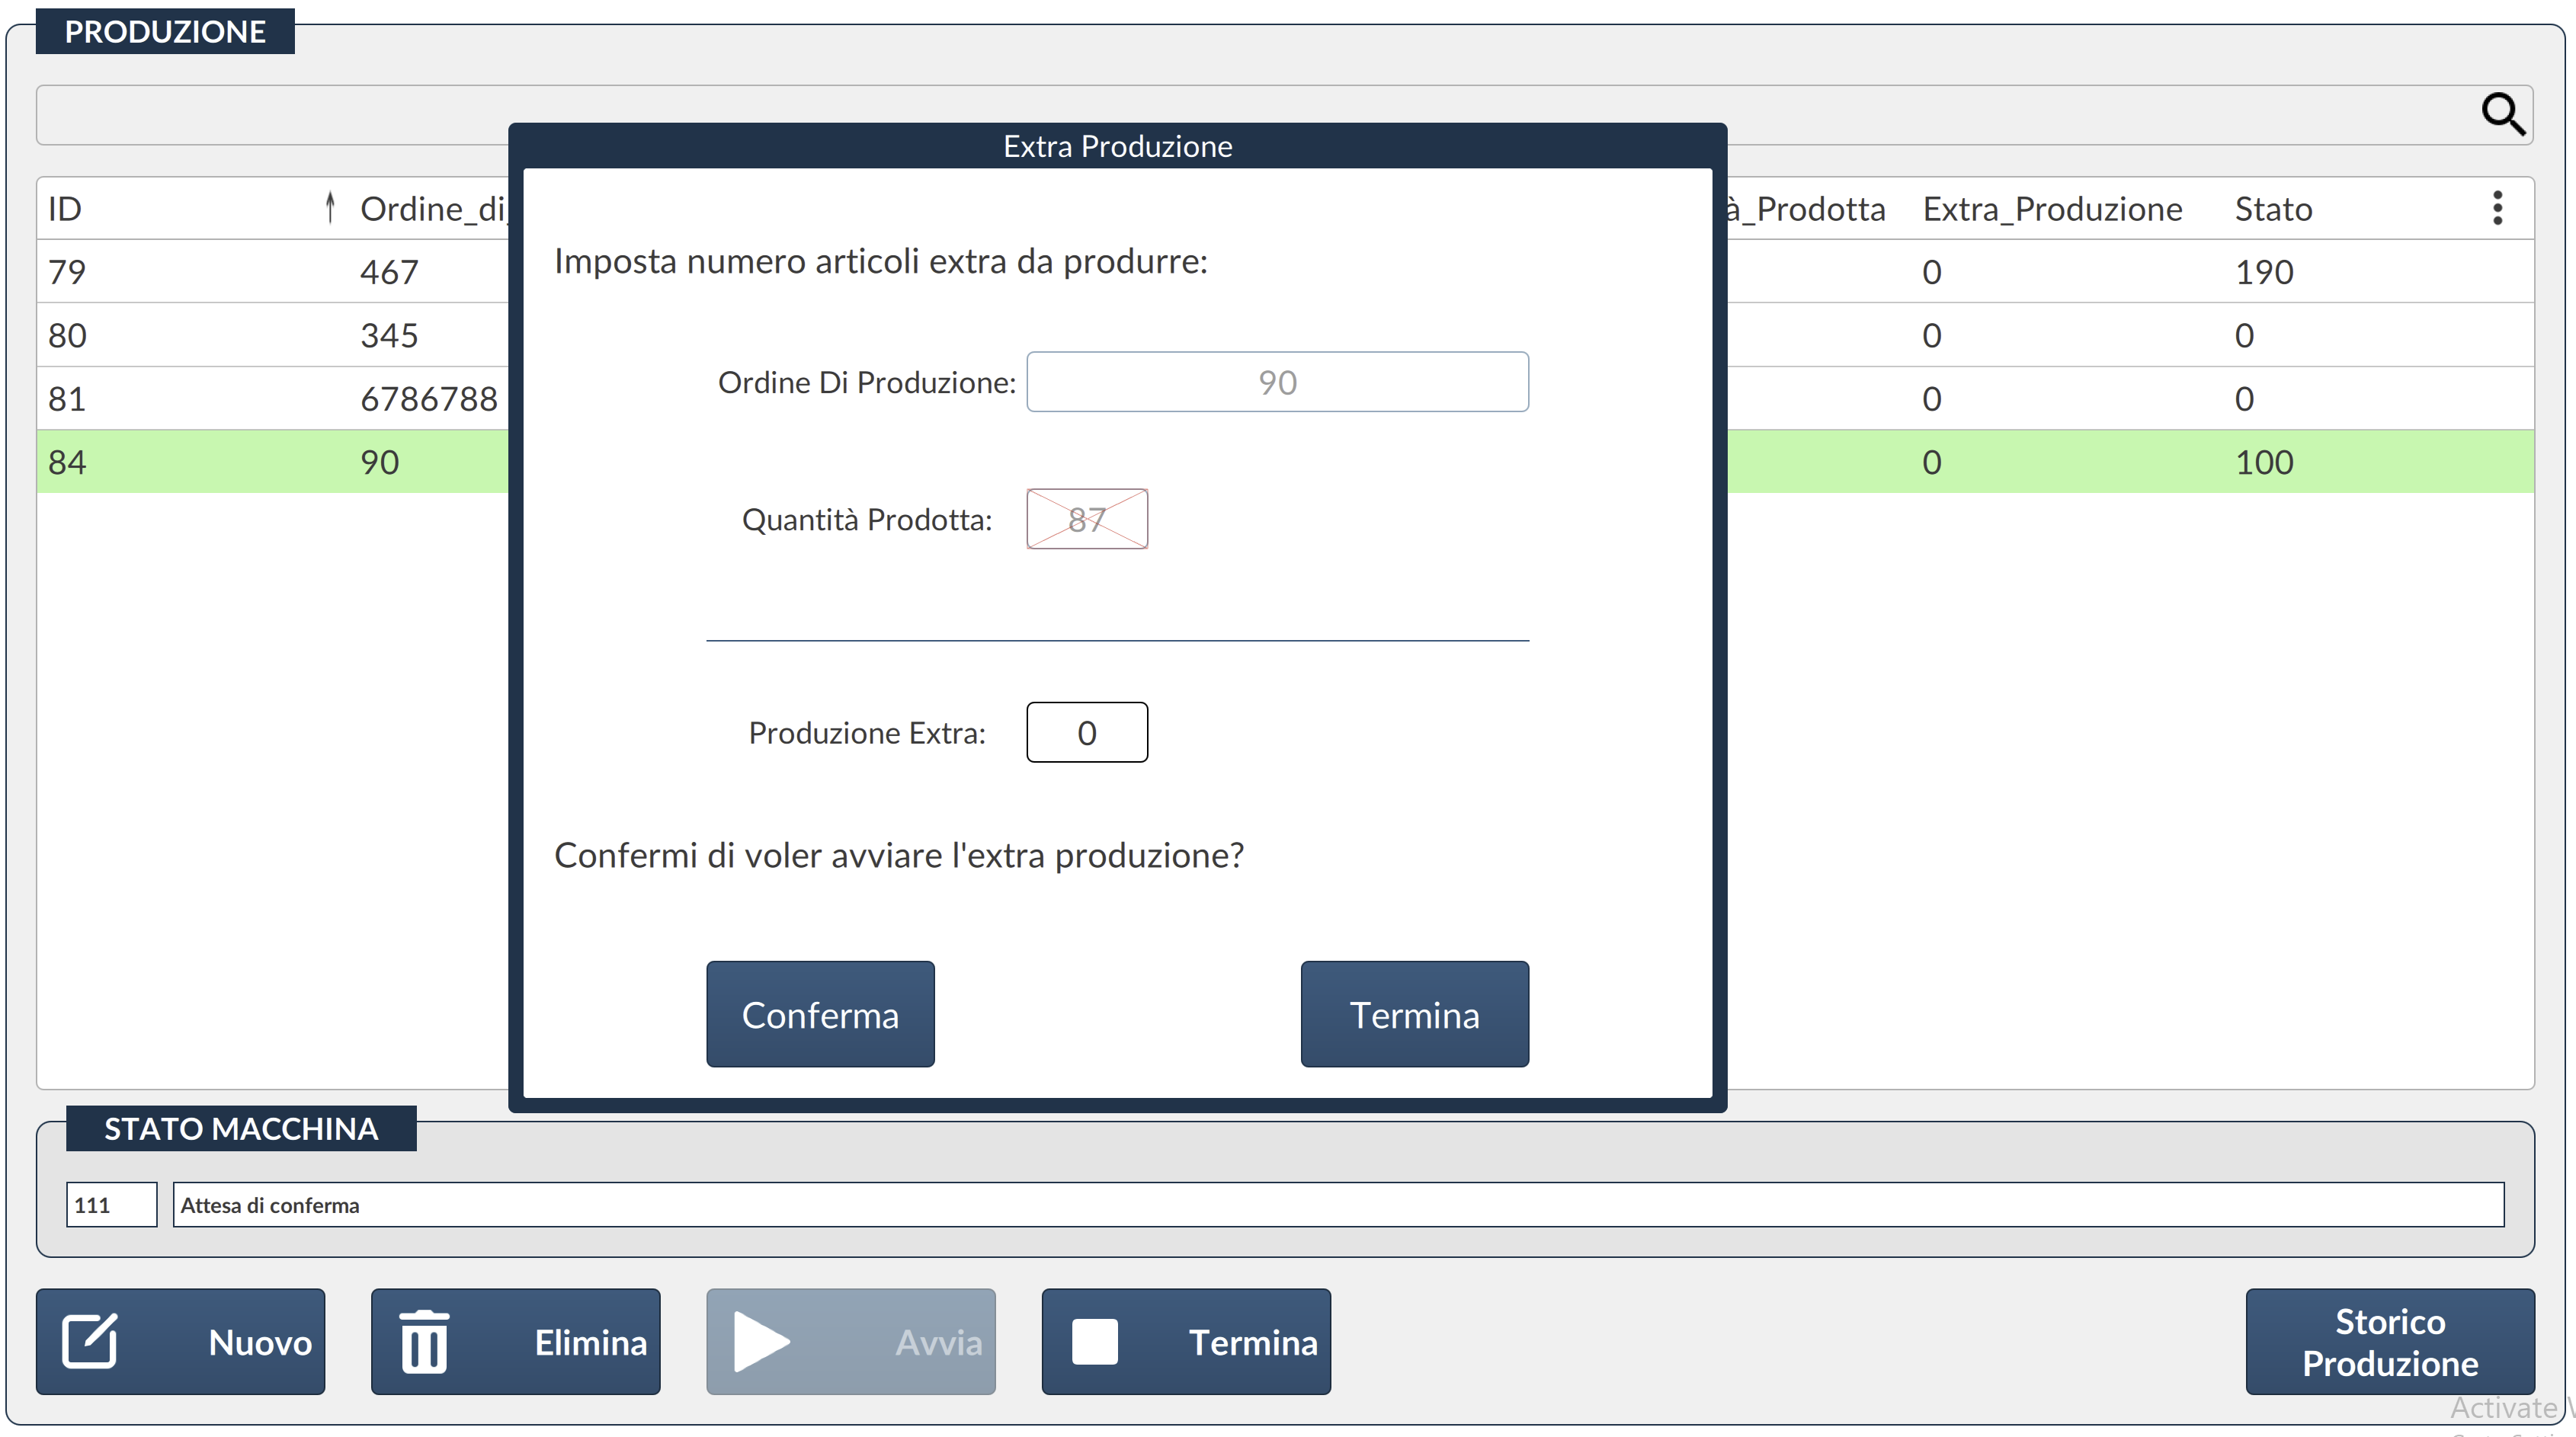
\includegraphics[width=1\linewidth]{Immagini/ExtraProduzione.png}
    \caption{Esempio richiesta di \textit{Extra Produzione}}
    \label{fig:Extraproduzione.png}
\end{figure}

Passiamo ora a due iterazioni principali nello SCADA: \textit{Avvia Produzione} e \textit{Termina Produzione}. Nel caso di \textit{Avvia Produzione}, dopo aver dato conferma tramite apposito popup di verifica, viene richiamata la funzione \verb|pr_AvviaLocale|, che si occupa di configurare in autonomia le variabili fondamentali della produzione, permettendo alla macchina a stati di poterne usufruire:

\begin{csharp}
...
    /// <summary>
    /// Avvia produzione
    /// </summary>
    [ExportMethod]
    public void pr_AvviaLocale(long id)
    {
        Project.Current.GetVariable(VariablePaths.PathOdlStart).Value = id;
        Project.Current.GetVariable(VariablePaths.Pathap_start).Value = true;
    }
...
\end{csharp}

Per quanto riguarda \textit{Termina Produzione} invece, viene semplicemente impostata la variabile \verb|pr_ButtonTerminaSelected = TRUE|, invocando la macchina a stati. Quest'ultima, nel passo corrispondente, richiama la funzione \verb|pr_TerminateAllRunningLocale|, che si occupa per spostare l'ordine nello storico della produzione. Nella funzione indicata e successivamente illustrata, il sistema procede dapprima ad individuare l'ordine con lo stato 160 "di aggiornamento tabelle e spostamento nello storico" (righe 8-9). Poi, una volta trovato l'ordine, viene creato un nuovo oggetto temporaneo in cui vengono inseriti tutti gli attributi dell'ordine, con l'aggiunta della data di terminazione della produzione (da riga 17 a riga 25). Infine, l'oggetto risultante viene trasferito nella tabella di \textit{Storico Produzione} (riga 28).

\begin{csharp}
...
    /// <summary>
    /// Recupera i dati delle produzioni terminate e li sposta nello storico
    /// </summary>
    public void pr_TerminateAllRunningLocale()
    {
        object[,] result;
        _store = Project.Current.Get<Store>(DATASTORE_DATABASE);
        _store.Query($"SELECT * FROM {TABLE_NAME} WHERE \"/Status\" = 160", out _, out result);
    
        if (result.GetLength(0) == 0 || result.GetLength(1) == 0)
        {
            Log.Warning("pr_TerminateAllRunning no record found");
            return;
        }
    
        ReaToClienteLocale prod = new ReaToClienteLocale();
        prod.Production_Command = "" + result[0, 0];
        prod.Product_ID = (string)result[0, 3];
        prod.dt_start = (DateTime?)result[0, 4];
        prod.dt_end = DateTime.Now;
        prod.Quantity_Requested = (long)result[0, 8];
        prod.Quantity_Produced = (long)result[0, 9];
        prod.Total_Reject = (long)result[0, 11];
        prod.Extra_Production = (long)result[0, 10];
    
        _storicoprod = new RuntimeNetLogicReaToClienteStoricoLocale();
        _storicoprod.sp_InsertLocale(prod);

    }
...
\end{csharp}

\subsection{Storici Produzione/Allarmi}
Lo storico di produzione risulta accessibile tramite pulsante apposito, inserito nell'interfaccia di \textit{Produzione}. Al suo interno è stata progettata un'interfaccia simile a quella di \textit{Produzione}, ma con alcune differenze. Nello specifico, non è presente nessun pulsante per l'interazione diretta con la macchina, ma solo un \textit{DataGridView} che mostra tutte le informazioni sugli ordini prodotti. Difatti, le uniche iterazioni disponibili avvengono tramite un filtro di ricerca simile a quelli già trattati in precedenza, con l'aggiunta della possibilità di effettuare ricerche basate su data, o su un determinato periodo di tempo. La popolazione di questa tabella avviene solamente tramite la funzione analizzata nella sezione precedente, seguendo pressoché lo stesso approccio utilizzato per l'interfaccia di \textit{produzione}. Per quanto riguarda la parte back-end, è stato dapprima creato un \textit{RecipeSchema} contenente gli attributi necessari e, successivamente, sulla base del \verb|RuntimeNetLogic| fornito, è stata implementata la funzione di inserimento nel database \verb|sp_InsertLocale|. Questa funzione, come già descritto nelle sezioni precedenti, si occupa di inserire l'oggetto \verb|prod|, completo di tutti i suoi attributi nella tabella dello storico.

\begin{figure} 
    \centering
    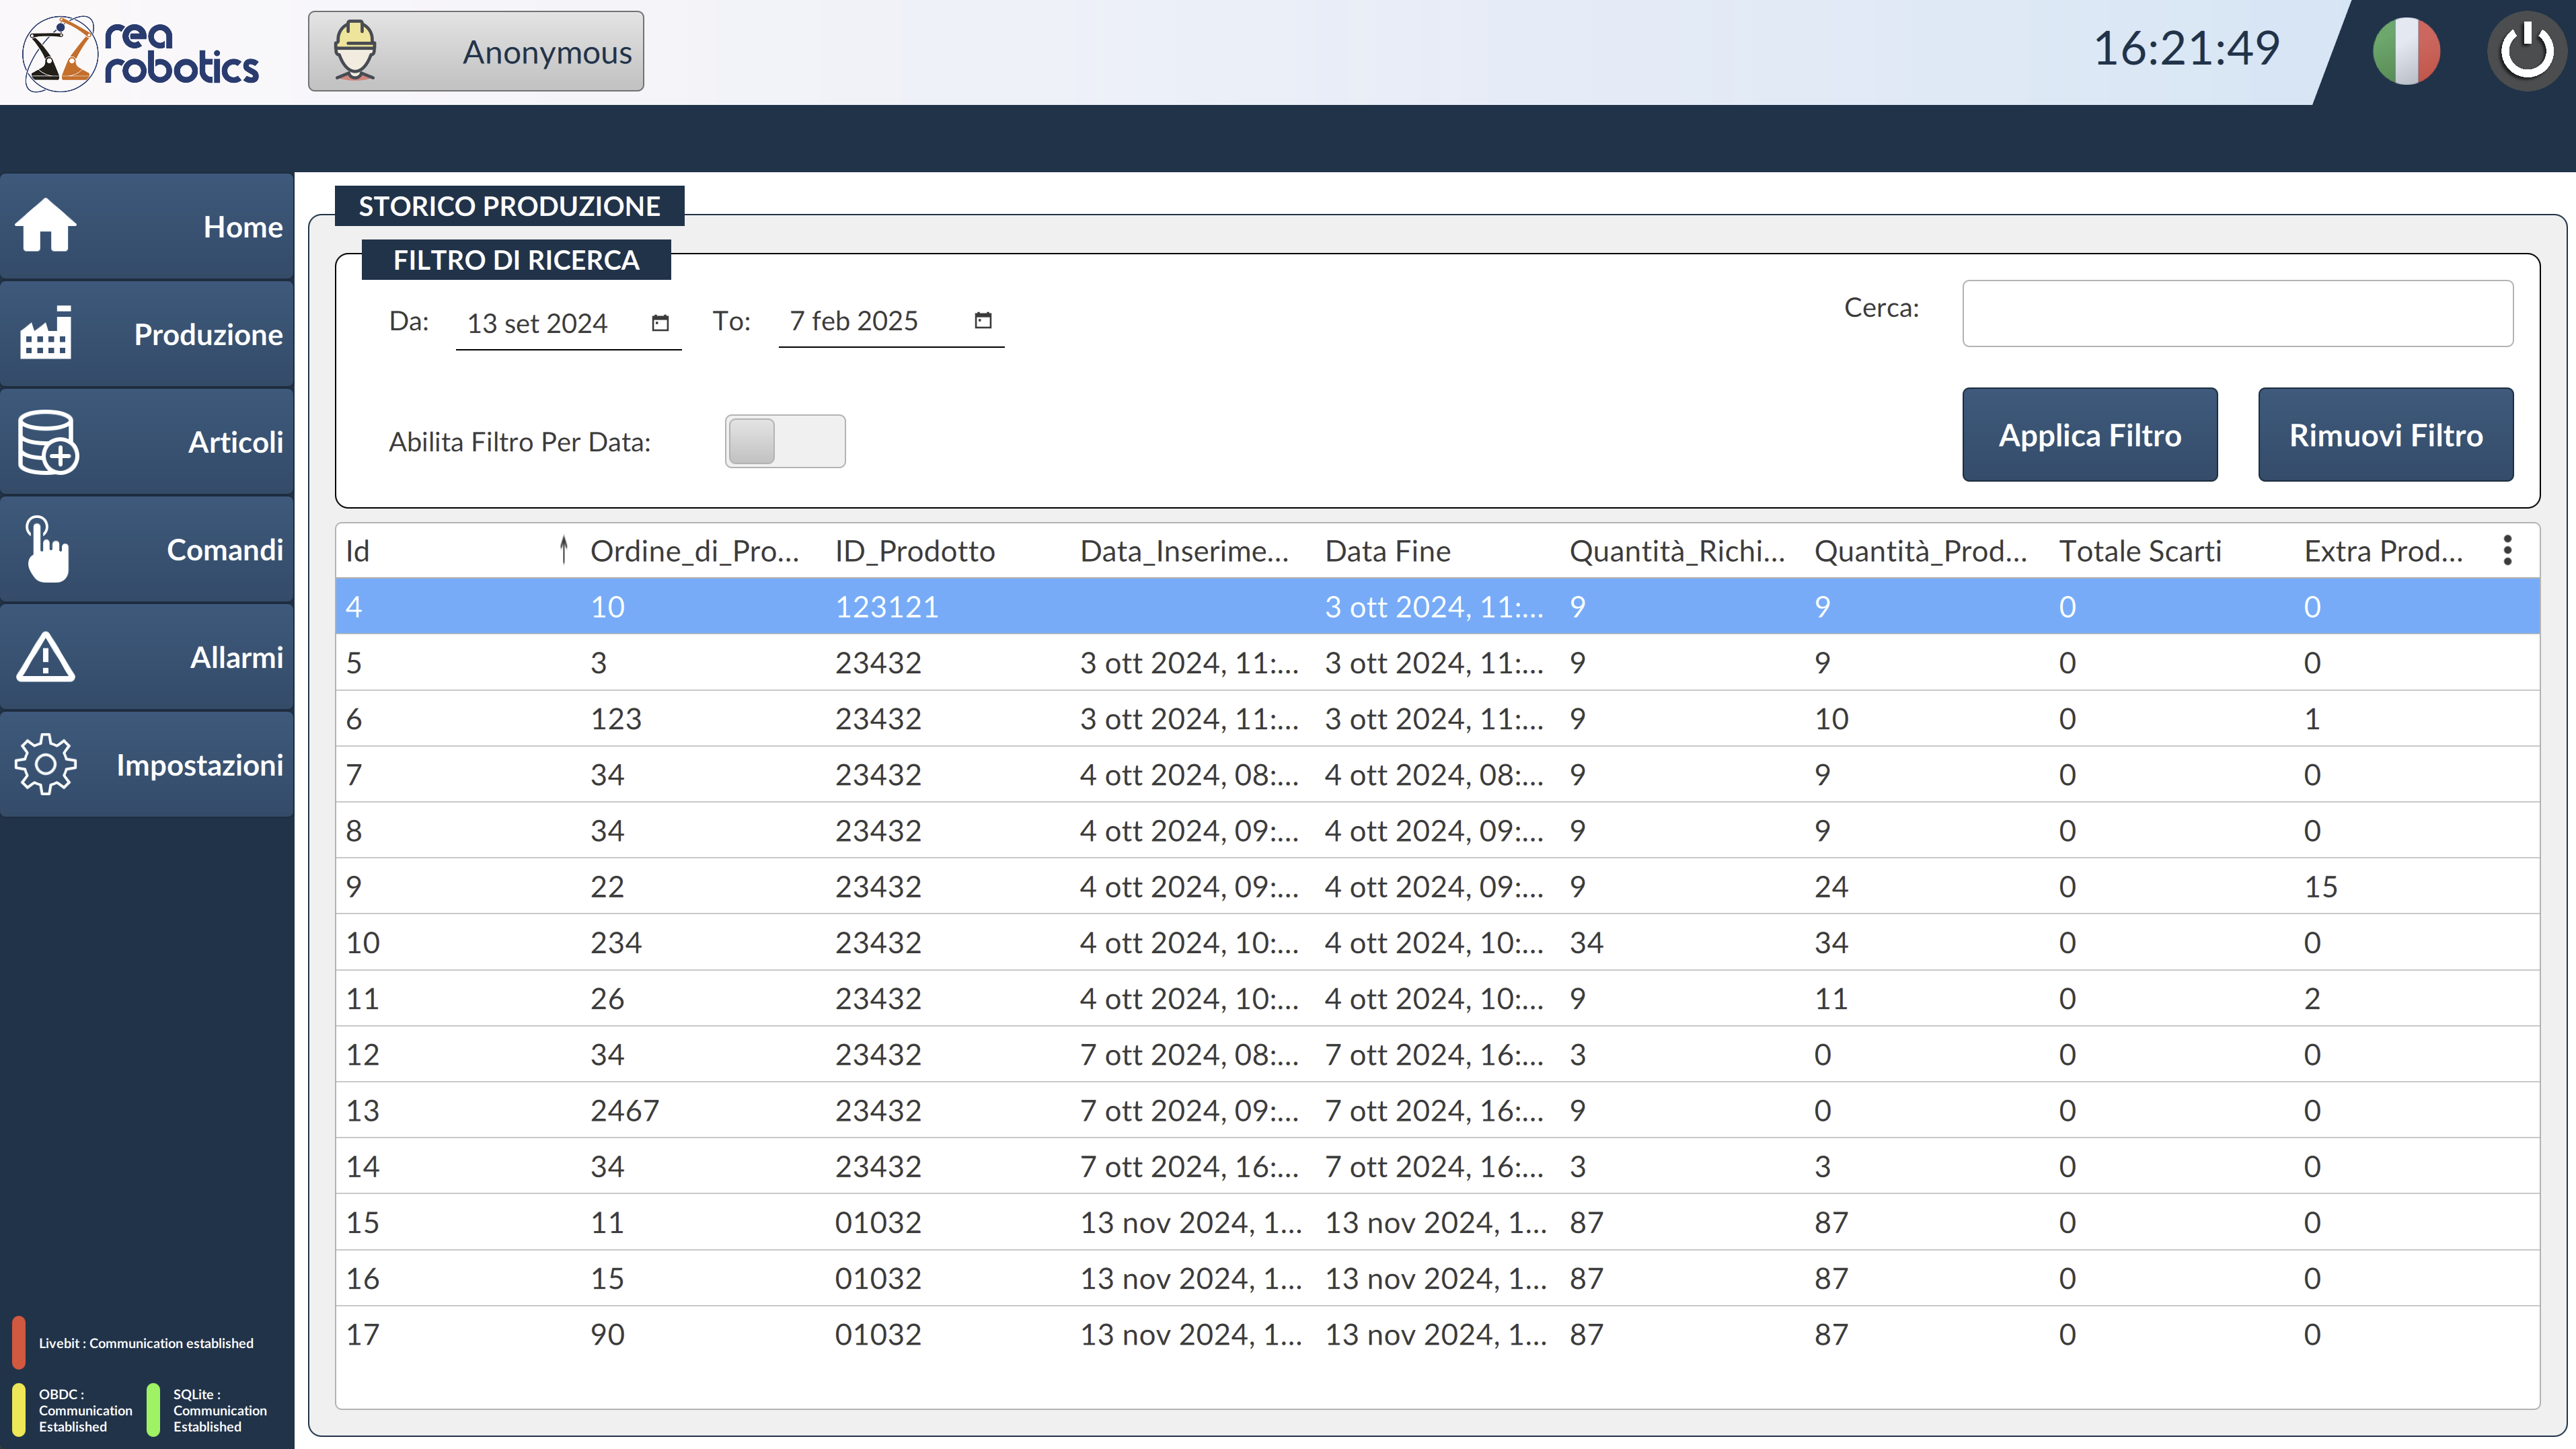
\includegraphics[width=1\linewidth]{Immagini/StoricoProduzione.png}
    \caption{Illustrazione sezione \textit{Storico Produzione}}
    \label{fig:StoricoProduzione.png}
\end{figure}

\begin{csharp}
...
public class RuntimeNetLogicReaToClienteStoricoLocale : BaseNetLogic
{
    ... //Altro codice fornito da FT Optix

    /// <summary>
    /// Inserisce un record nello storico
    /// </summary>
    public void sp_InsertLocale(ReaToClienteLocale prod)
    {
        try
        {
            string[] columns = { "/Production_Command", "/Product_ID", "/dt_start", "/dt_end", "/Quantity_Requested", "/Quantity_Produced", "/Total_Reject", "/Extra_Production" };

            var values = new object[1, 8];
            values[0, 0] = prod.Production_Command;
            values[0, 1] = prod.Product_ID;
            values[0, 2] = prod.dt_start;
            values[0, 3] = prod.dt_end;
            values[0, 4] = prod.Quantity_Requested;
            values[0, 5] = prod.Quantity_Produced;
            values[0, 6] = prod.Total_Reject;
            values[0, 7] = prod.Extra_Production;

            _store = Project.Current.Get<Store>(DATASTORE_DATABASE);
            _table = _store.Tables.Get<Table>(TABLE_NAME);
            _table.Insert(columns, values);

        }
        catch (Exception ex)
        {
            Log.Warning($"ERROR: sp_InsertLocale {ex.Message}");
        }
    }

}
...
\end{csharp}

Per quanto riguarda la gestione degli allarmi\textsuperscript{\cite{factorytalk_alarms}}, ci sono diversi aspetti da analizzare. Innanzitutto, dal punto di vista progettuale sono stati creati due pannelli dedicati: uno per la visualizzazione della lista di allarmi e un altro per i warning attivi. Di seguito, la schermata rimane essenziale, includendo solamente i pulsanti per la gestione di alcuni allarmi e warning, oltre alla sezione di \textit{Storico Allarmi}. A differenza di altre sezioni, gli allarmi non vengono gestiti tramite database ma direttamente da FT Optix™. Infatti, all'interno della cartella di progetto è presente una sotto-cartella dedicata a contenere solamente allarmi e warning (\ref{fig:CartellaAllarmi.png}) dell'impianto. 

\begin{figure}[!ht]
    \centering
    \begin{subfigure}[t]{0.35\textwidth} % 45% della larghezza del testo
        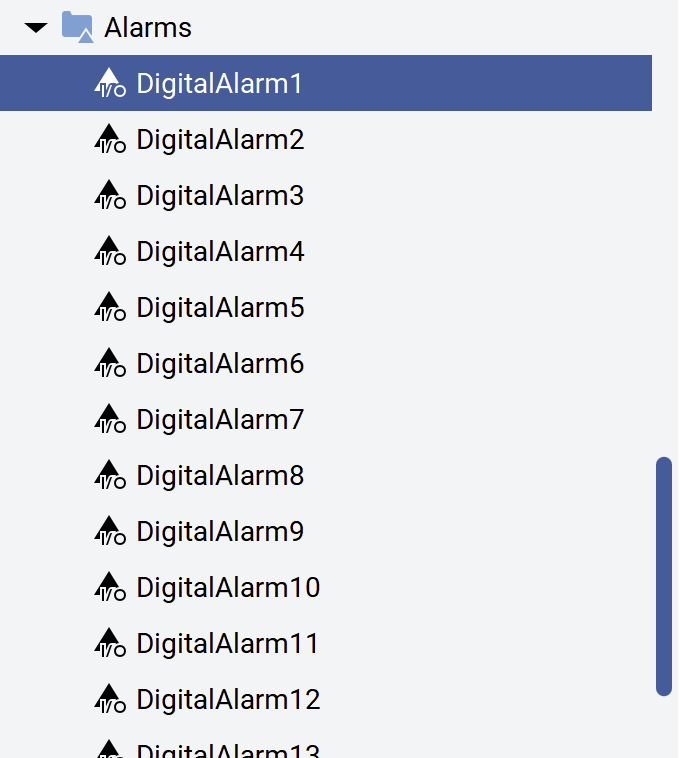
\includegraphics[width=\linewidth]{Immagini/CartellaAllarmi.png}
        \caption{Project view su \textit{Allarmi} in FT Optix™}
        \label{fig:CartellaAllarmi.png}
    \end{subfigure}
    \hfill
    % Seconda immagine
    \begin{subfigure}[t]{0.55\textwidth} % 45% della larghezza del testo
        \centering
        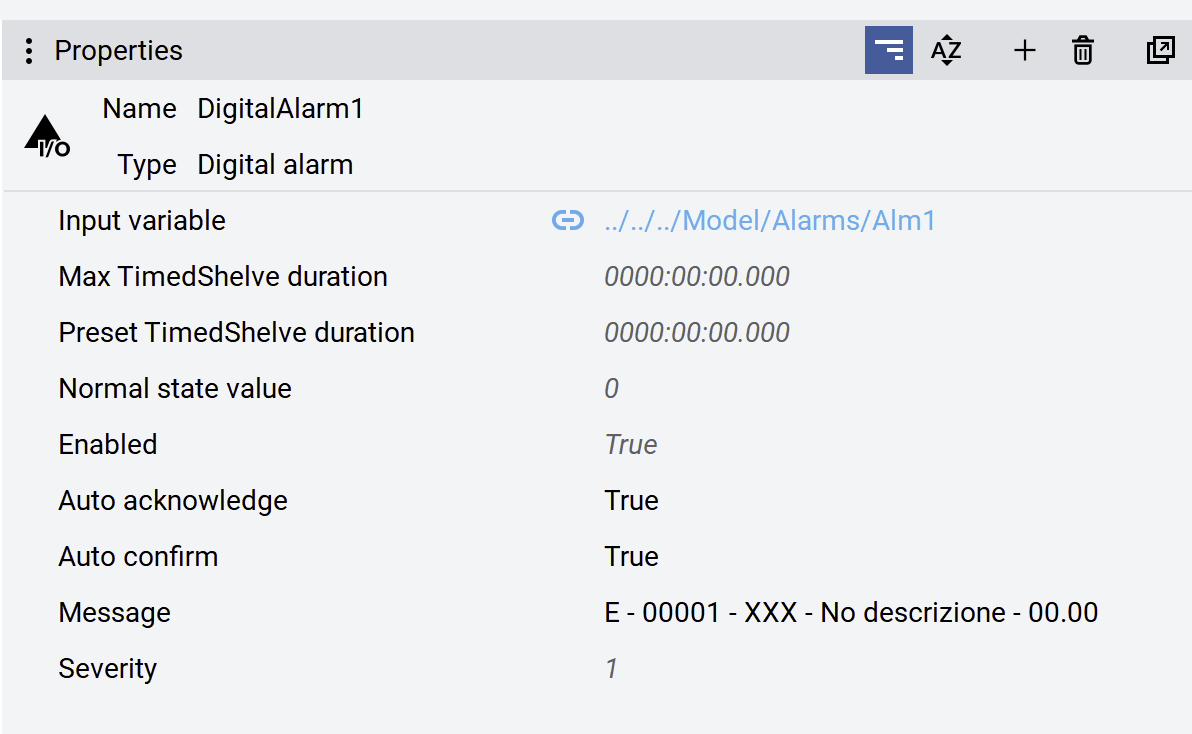
\includegraphics[width=\linewidth]{Immagini/AllarmiInfografica.png}
        \caption{Proprietà \textit{Allarmi}}
        \label{fig:AllarmiInfografica.png}
    \end{subfigure}
    \caption{Illustrazione pannelli presenti in FT Optix™}
    \label{fig:two-images00}
\end{figure}

Attraverso l'interfaccia di programma è, inoltre, possibile impostare diverse proprietà per ogni singolo allarme, come ad esempio il messaggio da visualizzare nello SCADA, la priorità e i tempi di visualizzazione del segnale (\ref{fig:AllarmiInfografica.png}). Tutta la parte di gestione degli allarmi viene poi effettuata da FT Optix™. Infine, se è necessario visualizzare i messaggi di allarme in altre sezioni, come ad esempio sul Pannello di Stato, è sufficiente richiamarli tramite funzioni specifiche di FT Optix™. In particolare, nel nostro caso, grazie alla libreria \verb|AllarmBannerlogic| il processo di visualizzazione degli allarmi viene automatizzato. Questo approccio permette di semplificare il lavoro, poiché è necessario solo inserire gli allarmi nella cartella di progetto. Naturalmente in sistemi SCADA più complessi è possibile lavorare manualmente tramite script sulla libreria, permettendo di personalizzare ulteriormente la gestione degli allarmi.

\begin{figure} [ht]
    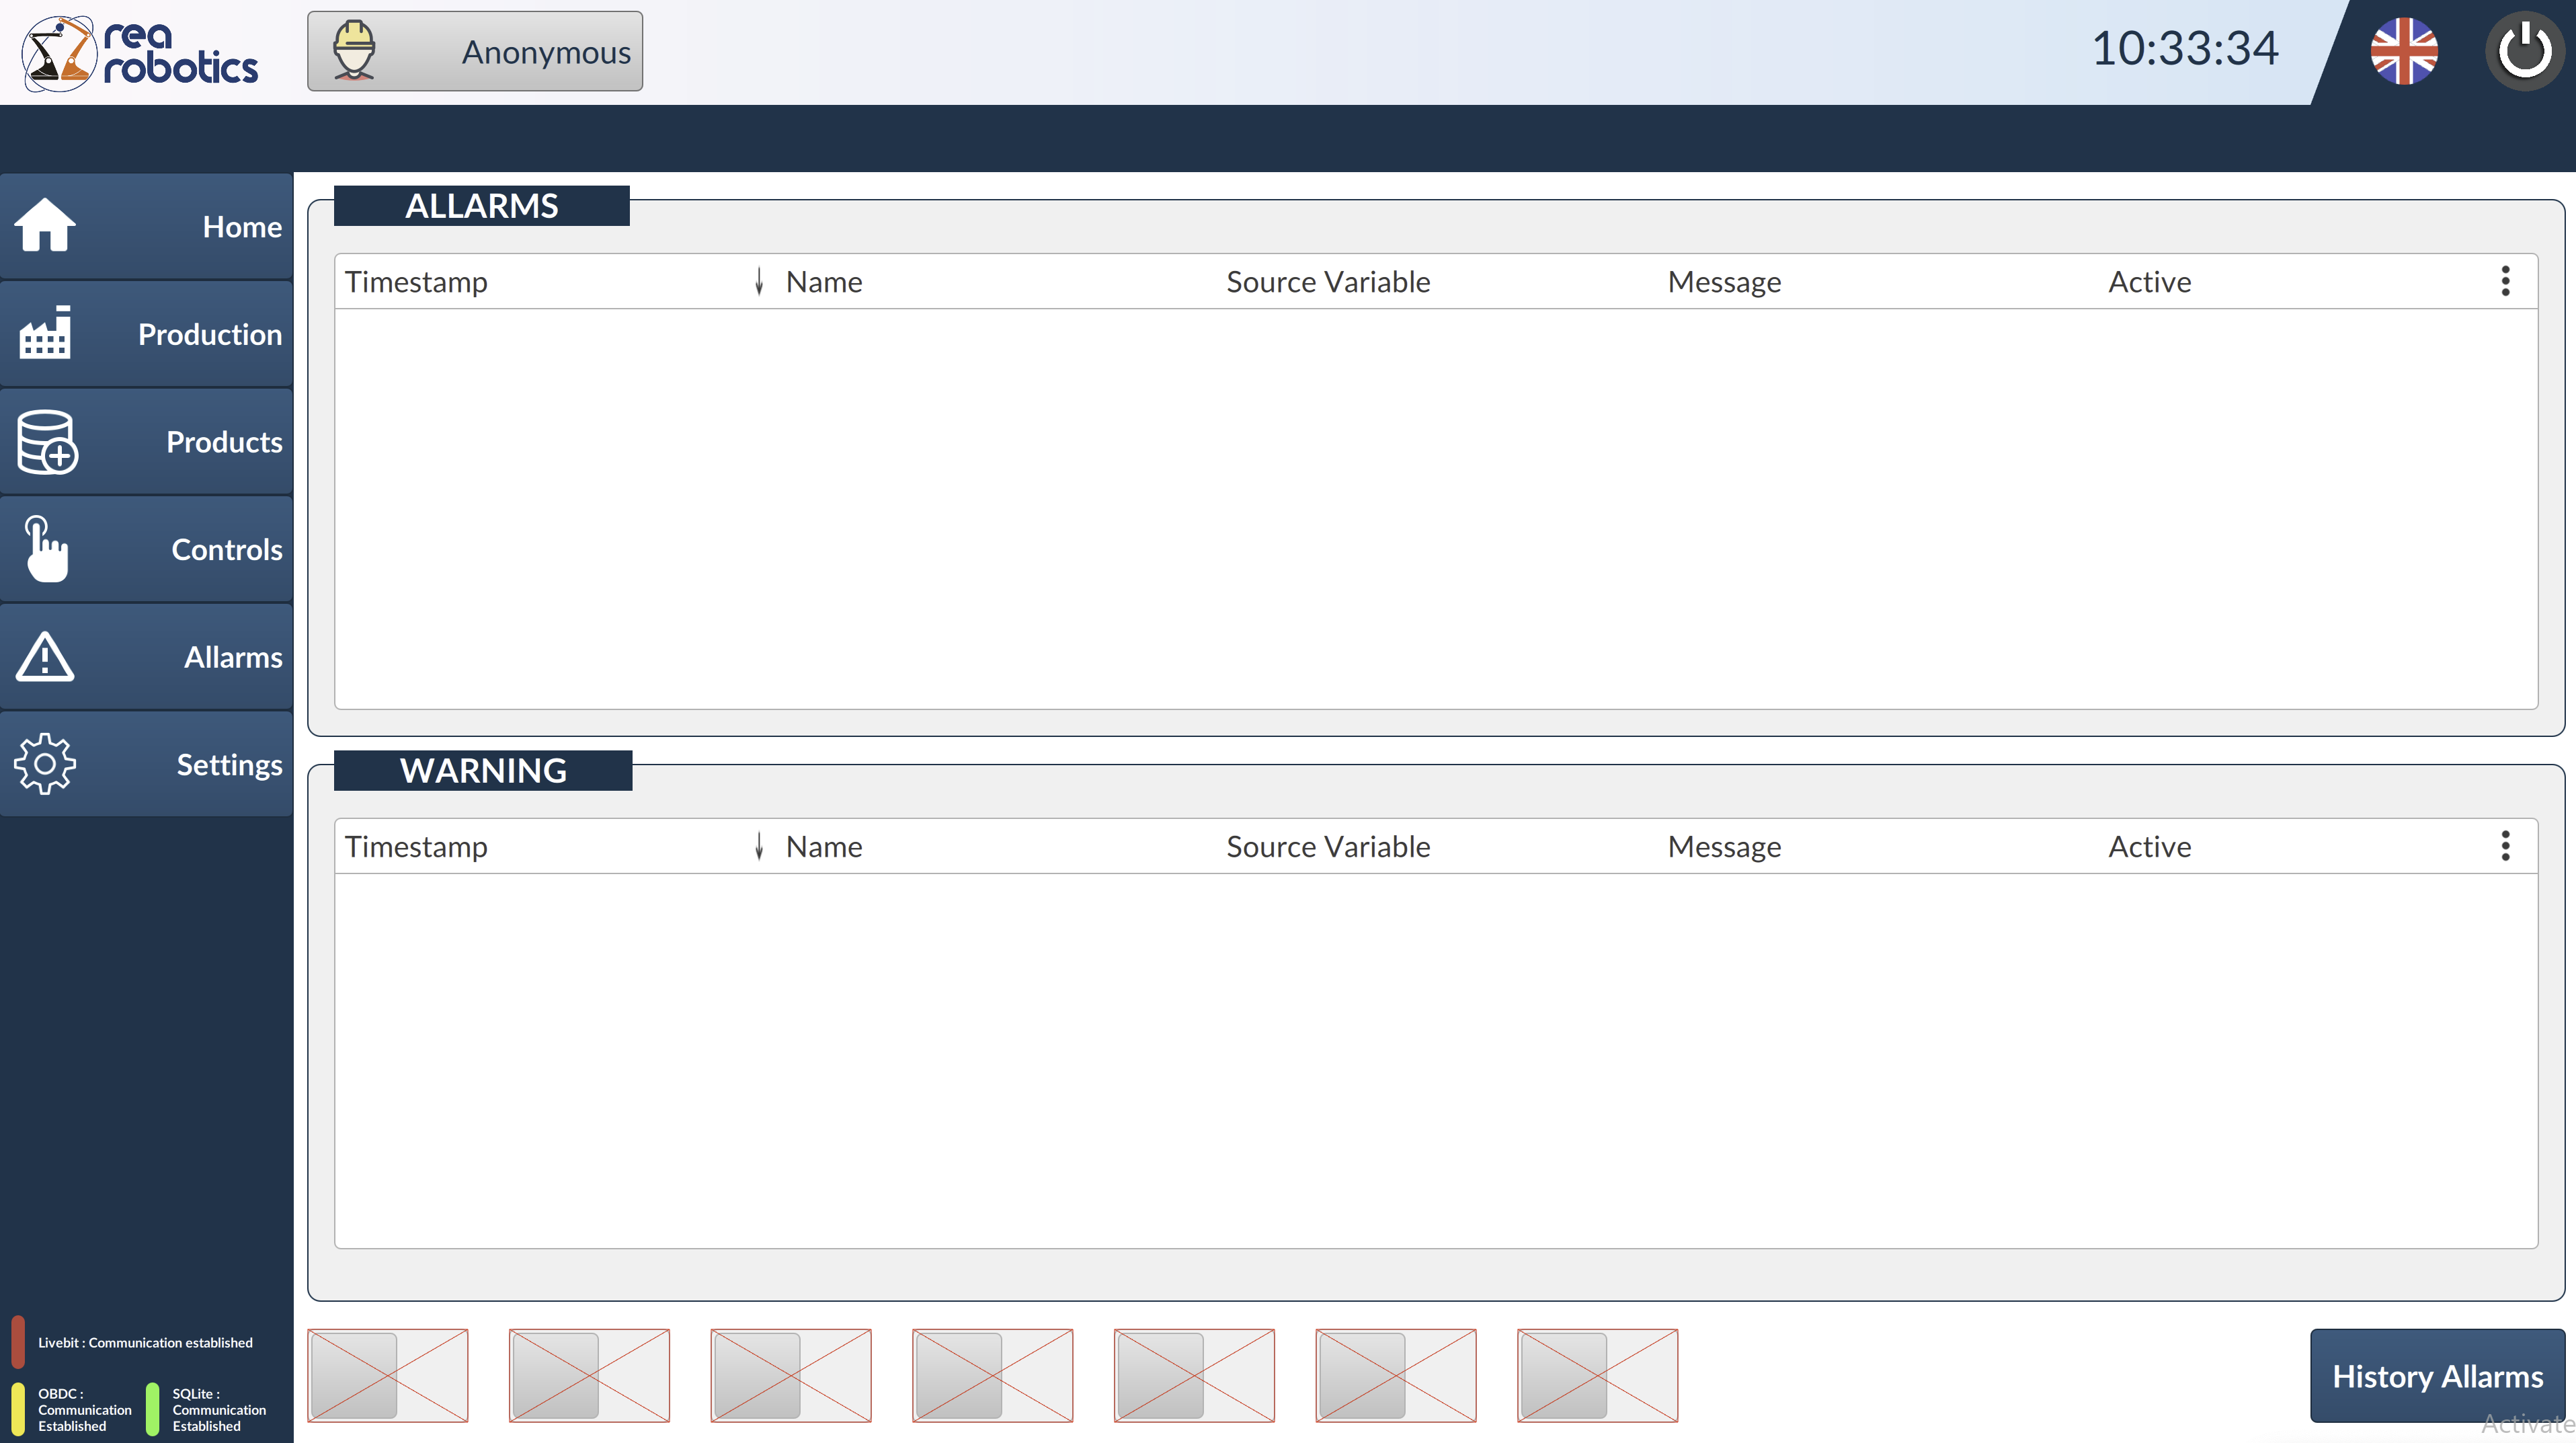
\includegraphics[width=\linewidth]{Immagini/Allarmi.png}
    \caption{Illustrazione sezione \textit{Allarmi}}
    \label{fig:Allarmi.png}
\end{figure}

\subsection{Configurazione Database aziendale}
Per quanto riguarda la parte di database aziendale, in questa sottosezione ci occuperemo della configurazione base di un database di tipo \verb|SQL Server|, come già visto per \verb|SQLite|. Inizialmente andiamo ad aggiungere all'interno della Project View, nella cartella DataStores, un oggetto di tipo \textit{ODBC database}\textsuperscript{\cite{factorytalk_odbcstore}}. A questo punto dobbiamo impostare sulle proprietà del database appena creato:
\begin{enumerate}
    \item Il DBMS type uguale a SQL Server.
    \item La struttura compresa dei vari campi delle tabelle, come già visto per \verb|SQLite|.
    \item Compilare i campi con le informazioni di accesso a SSMS
    \item Un \textit{DesignTimeNetLogic}, chiamato \verb|DesignTimeConfiguraDB| in cui andremo ad inserire informazioni fondamentali per l'utilizzo del database esterno.
\end{enumerate}
Successivamente non resta altro che replicare tutto ciò che è stato fatto per SQLite con le diverse variabili di modello, ricette e script specifici per far funzionare il database. Prima di passare al NetLogic di configurazione, è bene sottolineare che la scelta di utilizzare un database rispetto all'altro si trova all'interno della sezione Impostazioni, con la prima flag presente nel pannello. Grazie a questa flag viene cambiato il valore di una variabile booleana DB, impostando l'utilizzo delle tabelle corrette. Inoltre, questa variabile agisce sull'interfaccia di \textit{Produzione} e \textit{Articoli} visualizzata dall'operatore, che ha a disposizione due sezioni di facile utilizzo e comprensione per chi opera direttamente sul campo. Per quanto riguarda \verb|DesignTimeConfiguraDB|, è stata innanzitutto creata la classe con le costanti di riferimento del database:
\begin{csharp}
public class DesignTimeConfiguraDB : BaseNetLogic
{
    const string DB_SERVER = ".\\SQLEXPRESS";
    const string DB_NAME = "PRG_OPTIX";
    const string DB_USER = "sa";
    const string DB_PASSWORD = "reaSQL";

    private string _connectionString = $"Server={DB_SERVER};Database={DB_NAME};User Id={DB_USER};Password={DB_PASSWORD};";

    ...
\end{csharp}
Per poi configurare tramite il metodo \verb|ConfigureDB| l'accesso al database ed aggiungere eventuali tabelle necessarie al datastore OBDC di FT Optix™. Quindi, è stata copiata la libreria \verb|sni.dll| per fornire comunicazione con SQL Server, per poi aggiungere le tabelle necessarie:
\begin{csharp}
...
    sourcePath = Path.Combine(RuntimePath, "sni.dll");
    destinationPath = Path.Combine(RuntimePath, "NetSolution", "bin", "sni.dll");
    System.IO.File.Copy(sourcePath, destinationPath, true);
...
    //aggiungo le tabelle necessarie con le relative colonne
    List<string> tables = new List<string>();
    tables = ListTables();
    
    if (tables.Count>0 )
    {
        foreach (string tbl in tables)
        {
            AddNewTable(db, tbl);
        }
    }
...
\end{csharp}
Infine vengono gestiti i tipi di dati SQL, mappandoli correttamente:
\begin{csharp}
...
     static Type MapSqlType(string sqlType)
 {
     switch (sqlType.ToLower())
     {
         case "int":
             return typeof(int);
         case "varchar":
         case "nvarchar":
         case "char":
         case "nchar":
             return typeof(string);
         // Aggiungi altri casi secondo necessità
         default:
             return typeof(object); // Tipo generico per altri tipi non gestiti
     }
 }
\end{csharp}
Questo script automatizza la configurazione del collegamento ad un database SQL Server garantendo che le tabelle e le colonne siano mappate correttamente nell'ODBC dell’HMI. Nondimeno, lo script gestisce la copia delle librerie necessarie, le connessioni e soprattutto il recupero dinamico delle strutture delle tabelle, rendendo le tabelle facilmente scalabili.

\section{Sviluppo back-end e integrazione con il PLC}\label{sec:Sviluppo back-end e integrazione con il PLC}

In questa sezione analizziamo gli aspetti necessari per poter unire tutto ciò che è stato progettato finora. Lato back-end, dobbiamo garantire che lo SCADA comunichi correttamente con uno o più PLC, a seconda dell'impianto, ottenendo pieno controllo del sistema. Questo approccio permette di gestire qualsiasi caso d'uso o variabile che potrebbe comportarsi in modo imprevisto durante l'operatività della macchina. Ho deciso di focalizzare l'attenzione su due elementi chiave: la possibilità che lo SCADA determini esattamente il passo operativo del PLC in ogni momento, e la certezza che ci sia una comunicazione bidirezionale tra lo SCADA e il PLC. Per arrivare a ciò, è stata creata una macchina a stati, con un ciclo che inizia nel momento in cui la macchina viene avviata e che avanza esclusivamente in risposta ai segnali del PLC. Questa macchina rappresenta un'astrazione del comportamento del PLC, offrendo pieno controllo in qualsiasi momento. Il lavoro è stato suddiviso in più fasi:
\begin{enumerate}
    \item Inizializzazione di tutti i tag del PLC e dello SCADA.
    \item Sviluppo di un programma in grado di gestire tutti i casi d'uso e gli errori dell'impianto.
    \item Verifica che tutto sia coerente tra FT Optix™ e il Database.
\end{enumerate}

\subsection{Indicizzazione tag variabili}

L'idea a livello progettuale è stata di creare un contenitore, implementato sotto forma di classe, che raccogliesse tutti i percorsi delle variabili presenti su FT Optix™, inclusi quelli del PLC. Il primo passo consiste nell'identificare, su FT Optix™, tutte le variabili di nostro interesse. È fondamentale che sia attivata la modalità avanzata in FT Optix™ per eseguire i passi seguenti. Attraverso la \textit{Project View} vanno estrapolati i percorsi delle variabili. Ad esempio, consideriamo una variabile di modello scelta casualmente (\ref{fig:tag.png}). Una volta estratto il percorso, si ottiene una stringa di questo tipo: \verb|SCADA/Model/Produzione/ResetProduction|. Da quest'ultima conviene sempre escludere la prima parte del percorso, che rappresenta il nome del progetto, e utilizzare solo la parte rimanente. Questa scelta è motivata dal fatto che la prima parte, nel nostro caso: \verb|SCADA/| rappresenta il nome del Progetto, e se dovessimo riutilizzare tutto il modello in contesto multi-progetto, dovremmo aggiornarle globalmente tutte. Riducendo il percorso alla sola parte: \verb|Model/Produzione/ResetProduction|, si garantisce maggior flessibilità e portabilità. 

\begin{figure} [ht]
    \centering
    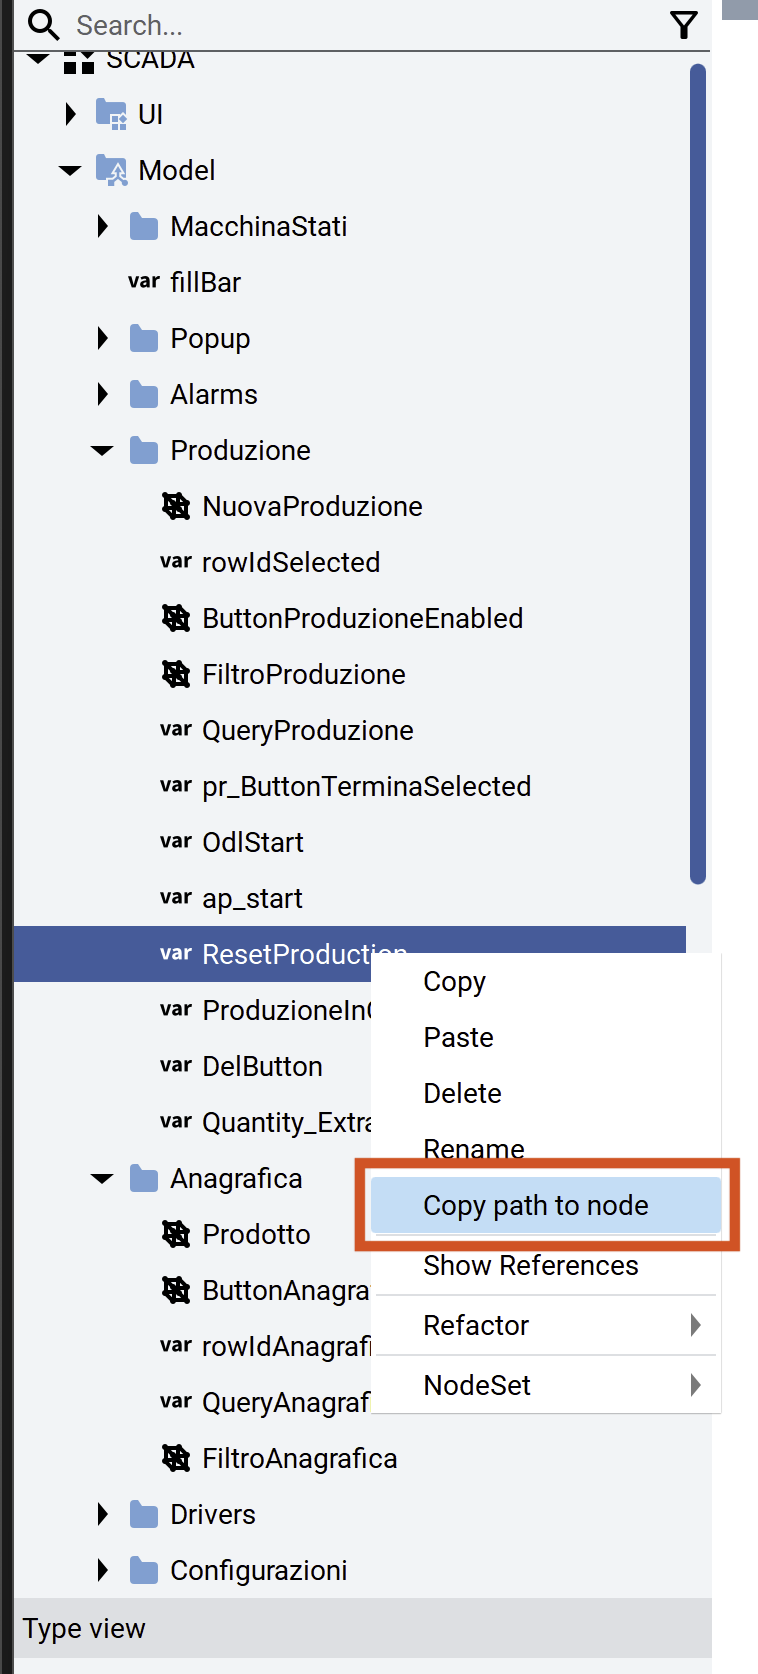
\includegraphics[width=0.3\linewidth]{Immagini/tag.png}
    \caption{esempio di salvataggio percorso variabile di modello}
    \label{fig:tag.png}
\end{figure}

Procediamo a creare la classe e ad inserire volta per volta tutti i percorsi delle variabili necessarie. Alla fine dovremmo ottenere una classe del genere:

\begin{csharp}
...

public static class VariablePaths
{
    ... // lista variabili per HMI

    //cliente_to_rea -> produzione
    public const string PathQueryProduzione                         = "Model/Produzione/QueryProduzione";
    public const string PathProduzioneFilterActive                  = "Model/Produzione/FiltroProduzione/FilterActive";
    public const string PathProduzioneTextFilter                    = "Model/Produzione/FiltroProduzione/TextFilter";
    public const string PathProduzioneAvviaEnabled                  = "Model/Produzione/ButtonProduzioneEnabled/AvviaEnabled";
    ...

    //rea_to_cliente -> storico
    public const string PathQueryStorico                            = "Model/Storico/QueryStorico";
    public const string PathStoricobdateFilter                      = "Model/Storico/bdateFilter";
    public const string PathStoricoDateFrom                         = "Model/Storico/DateFrom";
    public const string PathStoricoDateTo                           = "Model/Storico/DateTo";

    //anagrafica
    public const string PathQueryAnagrafica                         = "Model/Anagrafica/QueryAnagrafica";
    public const string PathAnagraficaFilterActive                  = "Model/Anagrafica/FiltroAnagrafica/FilterActive";
    public const string PathAnagraficaTextFilter                    = "Model/Anagrafica/FiltroAnagrafica/TextFilter";
    ...
    
    ... // lista variabili per HMI
\end{csharp}

Nella classe sono state inserite variabili secondo una precisa struttura: il percorso salvato in precedenza associato ad una stringa. Questo approccio consente maggiore controllo delle variabili all'interno della macchina a stati e, qualora sia necessario, permette di aggiungere nuove variabili semplicemente aggiornando la suddetta classe. È inoltre consigliato, ma non estremamente essenziale, suddividere le variabili secondo una logica ben definita in modo che siano facilmente rintracciabili, specialmente in impianti enormemente più strutturati.

Per la gestione delle variabili nella macchina a stati è stata definita una regola di suddivisione in due tipologie principali per fornire maggiore sicurezza:
\begin{enumerate}
    \item \textbf{DB92-PLCtoHMI}: sono tutte le variabili gestite dal controllore logico programmabile e inviate all'HMI, che le può leggere ma non modificare.
    \item \textbf{DB91-HMItoPLC}: variabili gestite sempre dal PLC, ma scrivibili solo dallo scada e leggibili dal PLC.
\end{enumerate}
Questa classificazione rimane costante indipendentemente dall'impianto; ciò che cambierà sono la quantità e il tipo di segnale dei tag. Nel caso specifico, verranno considerate le variabili utilizzate in un impianto di piegatura, che sarà analizzato più dettagliatamente nel capitolo \ref{sec:CasoStudio}. 

\subsection{Sviluppo Macchina a Stati}

 Dal lato progettazione, è stato inserito un oggetto \textit{RunTimeNetLogic} associato alla \textit{MainWindow}. Per quanto concerne la programmazione, lo script associato è stato suddiviso in diverse parti. Inizialmente, vengono dichiarati alcuni script strettamente legati al database, che vengono richiamati all'interno della \verb|StateMachine|. Successivamente, all'interno della funzione \verb|Start| (riga 19), è stata definita una \verb|PeriodicTask| con i seguenti attributi: 
 \begin{itemize}
     \item \verb|Maincycle|: contiene la logica periodica del sistema
     \item \verb|250ms|: indica la frequenza con cui la logica viene ripetuta periodicamente 
     \item \verb|LogicObject|: contiene le risorse necessarie per l'esecuzione.
 \end{itemize}
Grazie a questa configurazione, dopo aver avviato l'impianto, il maincycle viene eseguito ogni 250ms. Questa frequenza garantisce una sincronizzazione quasi istantanea tra HMI e PLC, riducendo al minimo gli errori.

\begin{csharp}
...
public class script_maincycle : BaseNetLogic
{
    private PeriodicTask myPeriodicTask;
    private RuntimeNetLogicClienteToRea _prod;
    private RuntimeNetLogicAnagrafica _art;

    private RuntimeNetLogicClienteToReaLocale _prodLocale;
    private RuntimeNetLogicAnagraficaLocale _artLocale;

    public override void Start()
    {
        _prod = new RuntimeNetLogicClienteToRea();
        _art = new RuntimeNetLogicAnagrafica();

        _prodLocale = new RuntimeNetLogicClienteToReaLocale();
        _artLocale = new RuntimeNetLogicAnagraficaLocale();

        myPeriodicTask = new PeriodicTask(Maincycle, 250, LogicObject);
        myPeriodicTask.Start();

    }

    public override void Stop()
    {
        myPeriodicTask.Dispose();
    }

    public void Maincycle()
    {
        StateMachine();
    }

    private void StateMachine()
    {
    ...
\end{csharp}

La struttura della\verb|StateMachine| è stata organizzata in diverse sezioni. La prima si occupa di inizializzare le variabili, richiamando i percorsi definiti nella classe \verb|VariablePaths| illustrata in precedenza, che contiene tutti i tag di interesse. Di seguito, una parte del codice illustrato:

\begin{csharp}
...
    private void StateMachine()
{
    //inizializzo variabili plc
    PopUpNetLogic popup                             = new PopUpNetLogic();
    var popupOK                                     = Project.Current.GetVariable(VariablePaths.PathPopupOK);
    var popupYes                                    = Project.Current.GetVariable(VariablePaths.PathPopupYes);
    var popupNo                                     = Project.Current.GetVariable(VariablePaths.PathPopupNo);

    var MachineStatusText                           = Project.Current.GetVariable(VariablePaths.PathMachineStatusText);
    var MachineStatus                               = Project.Current.GetVariable(VariablePaths.PathMachineStatus);
    var OdlStart                                    = Project.Current.GetVariable(VariablePaths.PathOdlStart);
    long OdlStartLong                               = OdlStart.Value; 
    var ap_start                                    = Project.Current.GetVariable(VariablePaths.Pathap_start);
    var pr_ButtonTerminaSelected                    = Project.Current.GetVariable(VariablePaths.Pathpr_ButtonTerminaSelected);
    var ResetProduction                             = Project.Current.GetVariable(VariablePaths.PathResetProduction);
    var ProduzioneInCorso                           = Project.Current.GetVariable(VariablePaths.PathProduzioneInCorso);

    var DB91_CambioProduzione                       = Project.Current.GetVariable(VariablePaths.PathDB91_CambioProduzione);
    var DB91_TerminaProduzione                      = Project.Current.GetVariable(VariablePaths.PathDB91_TerminaProduzione);
    ... // altre variabili plc
\end{csharp}
Dopo l'indicizzazione, la macchina stati è composta da vari passi definiti all'interno di uno \verb|switch-case| e numerati da 0 a 199, ciascuno per uno specifico stato operativo. Questo approccio logico è ampiamente utilizzato negli impianti industriali in REA, in quanto consente di gestire in modo modulare e scalabile le varie operazioni dallo scada oltre a facilitare la manutenzione futura. Di seguito, una panoramica dei passi standard:
\begin{itemize}
    \item \verb|0 = "Inizializzazione"|: passo che identifica l'avvio della macchina, solitamente corrisponde alla schermata di caricamento dell'HMI.
    \item \verb|1 = "Stato iniziale (IDLE)"|: passo in cui avviene un reset completo delle variabili HMI e DB91.
    \item \verb|10 = "Controllo allineamento con PLC-SCADA"|: sincronizzazione tra SCADA e PLC.
    \item \verb|20 = "Attesa avvio produzione"|: stato di attesa, con macchina operativa per la produzione.
    \item \verb|70 = "Attesa esito da PLC - ok/ko"|: attesa del segnale di risposta dal PLC dopo un comando inviato dall'HMI.
    \item \verb|80 = "Attesa RESET segnali da PLC - ok/ko"|: verifica di sicurezza, attesa ulteriore segnale dal PLC.
    \item \verb|100 = "IN LAVORO"|: identifica che l'impianto è in piena attività produttiva.
    \item \verb|150 = "Fine produzione + attesa handshake PLC"|: stato di attesa del segnale di handshake da parte del PLC.
    \item \verb|165 = "Attesa reset richiesta termina produzione dal PLC"|: pulizia delle variabili per garantire la sicurezza operativa.
    \item \verb|190 = "ANNULLAMENTO CARICAMENTO DA OPERATORE"| annullamento di qualsiasi produzione attiva o in chiusura.
    \item \verb|199 = "Termina produzione completata correttamente"| controllo finale e ritorno al passo 20.
\end{itemize}
Come si può notare, non tutti i passi seguono un ordine sequenziale; questo consente di aggiungere eventuali estensioni future agli impianti. Partiamo con l'analizzare il codice di tutti i passi principali, escludendo l'implementazione di alcuni per l'impianto di piegatura, che analizzeremo successivamente nel capitolo \ref{sec:CasoStudio}.

Il codice di \verb|case 0| rappresenta la prima iterazione del ciclo e quindi l'avvio della macchina. Qui si gestisce il caricamento iniziale, inclusa l'interfaccia HMI. Viene monitorata la variabile \verb|fillBar|, cioè la barra di caricamento, per verificare che l'intero programma sia caricato (righe 7-10). Una volta completato il caricamento, lo stato viene impostato a 1, e nell'HMI viene caricata la pagina iniziale completa di tutta l'interfaccia (righe 13-20). Infine esce dal passo.
\begin{csharp}
...
    case 0:
        //-------------------------------------------
        MachineStatusText.Value = "Inizializzazione";
        //-------------------------------------------
    
        if (Project.Current.GetVariable("Model/fillBar").Value <15)
        {
            Project.Current.GetVariable("Model/fillBar").Value += 1;
        }
        else
        {
            MachineStatus.Value = 1;
            
            //cambia pagina
            var myPanel = LogicObject.GetPanelLoader("PanelLoader1");
            myPanel.ChangePanel("Main");
    
            var mainPanel = LogicObject.GetPanelLoader("PanelLoaderScreens");
            mainPanel.ChangePanel("Home");
        }
    
        break;
...
\end{csharp}
Il \verb|case 1| rappresenta uno dei passi più critici, poiché si occupa di controllare variabili, allarmi e sensori sia dell'HMI che del PLC. Questo passo è importante per garantire continuità in caso di blackout o spegnimenti anomali del pannello HMI, che potrebbero de sincronizzare PLC-SCADA. Al suo interno vengono eseguiti i seguenti reset:
\begin{enumerate}
    \item \verb|DB91_CambioProduzione.Value|: impostato a false (riga 7).
    \item \verb|ResetHMIProductVar()|: richiama la funzione di reset delle variabili HMI di produzione (riga 10).
    \item \verb|ResetPLCProductVar()|: richiama la funzione di reset delle variabili PLC (riga 13).
\end{enumerate}
Concluso il reset, la macchina imposta il passo successivo, cioè 10, ed esce dal passo (riga 15).
\begin{csharp}
...
    case 1:   
        //------------------------------------------------
        MachineStatusText.Value = "Stato iniziale (IDLE)";
        //------------------------------------------------
    
        DB91_CambioProduzione.Value = false;
    
        //Reset di tutte le variabili legate al caricamento programma su HMI
        ResetHMIProductVar();
    
        //Reset variabili PLC DB91
        ResetPLCProductVar();
    
        MachineStatus.Value = 10;
    
        break;
...
\end{csharp}
Dal \verb|case 10| tutto il codice è stato strutturato con l'implementazione sia per il database locale, sia per il database aziendale. Tuttavia, in questa spiegazione ci concentriamo su una singola implementazione, poiché le logiche principali rimangono identiche. Per prima cosa avviene un check sulla variabile \verb|DBExpress.Value| configurata nelle impostazioni dell'HMI che determina quale database è in utilizzo (riga 7). Fatto questo avviene un confronto diretto con la variabile di status nel PLC (riga 17): se maggiore di 0, il PLC sta già lavorando ad un ordine. In questo caso, tutte le variabili dello SCADA vengono aggiornate per riallinearsi con il PLC e continuare la produzione senza problemi (righe 20-29); se invece \verb|DB92_ODP.Value| è uguale a zero, il sistema procede al passo successivo senza ulteriori azioni (riga 33). 
\begin{csharp}
...
    case 10:
    //---------------------------------------------------------------
    MachineStatusText.Value = "Controllo allineamento con PLC-SCADA";
    //---------------------------------------------------------------

    if (DBExpress.Value)
    {
       ... //implementazione per SSMS
    }
    else
    {
        //sincronizzo il campo /Status con lo stato corretto dell'ordine che sta girando sul PLC
        _prodLocale.pr_StatusSyncro_Locale(DB92_ODP.Value);

        //se in plc sto lavorando con una ricetta allineo tabella in running
        if (DB92_ODP.Value > 0)
        {
            //Sincronizzo OdlStart
            OdlStartLong = DB92_ODP.Value;

            //mando prodotti al plc
            SendProductDataToPLCLocale(OdlStartLong);

            //mi metto in produzione in corso 
            ProduzioneInCorso.Value = true;

            //vado in produzione
            MachineStatus.Value = 100;
        }
        else
        {
            MachineStatus.Value = 20;
        }
    }

    break;
...
\end{csharp}
Il \verb|case 20| rappresenta lo stato in cui l'impianto è in attesa avvio produzione, monitorando continuamente le seguenti variabili (riga 12): 
\begin{itemize}
    \item \verb|ap_start.Value|: è stato avviato un ordine dall'operatore.
    \item \verb|OdlStartLong|: è maggiore di zero se esiste un ordine di produzione in attesa.
\end{itemize}
Se avvengono queste condizioni, i dati relativi all'ordine vengono inviati al PLC tramite funzione \verb|SendProductDataToPLCLocale| (riga 15). Se avviene l'invio, viene impostata \verb|ProduzioneInCorso.Value| a TRUE (riga 18), con  cambio al passo successivo (riga 21). In caso contrario viene aperto un popup di avvertimento e conseguentemente cambiato il passo (righe 26, 27).
\begin{csharp}
...
    case 20:
    //--------------------------------------------------
    MachineStatusText.Value = "Attesa avvio produzione";
    //--------------------------------------------------
    if (DBExpress.Value)
    {
        ... //implementazione per SSMS
    }
    else
    {
        if (ap_start.Value && OdlStartLong > 0)
        {
            //mando dati al plc
            if (SendProductDataToPLCLocale(OdlStartLong))
            {
                //vado in produzione in corso
                ProduzioneInCorso.Value = true;

                //cambio stato
                MachineStatus.Value = 25;
            }
            else
            {
                //Dati anagrafica non esistenti, popup e KO diretto
                popup.OpenPopUp("Dati anagrafica non esistenti: crea prima l'articolo in Anagrafica", 0);
                MachineStatus.Value = 21;
            }
        }
    }
    
    break;
...
\end{csharp}
Il \verb|case 21| gestisce l'attesa di lettura del popup da parte dell'operatore, procedendo al ripristino delle variabili di produzione e al cambio del passo. Nel \verb|case 25| viene impostata la variabile di cambio produzione a TRUE (riga 13), per avvisare il PLC del cambio di ordine. Viene aggiornato l'attributo dello stato dell'ordine nel database (riga 16), e viene richiamata la funzione per abilitare/disabilitare i pulsanti della schermata di produzione. Infine cambiamo passo (riga 19).
\begin{csharp}
...
    case 25:
    //---------------------------------------------------------
    MachineStatusText.Value = "Invio cambio produzione al PLC";
    //---------------------------------------------------------
    if (DBExpress.Value)
    {
        ... //implementazione per SSMS
    }
    else
    {
        //Handshake PLC - attendo risposta
        DB91_CambioProduzione.Value = true;

        //Aggiorno stato in db
        _prodLocale.pr_UpdateStatusLocale(OdlStartLong, MachineStatus.Value);

        //Aggiorno pulsanti
        _prodLocale.pr_ManageProductionButtonsLocale(MachineStatus.Value);

        //Cambio stato
        MachineStatus.Value = 50;
    }

    break;
...
\end{csharp}
I passi \verb|case 50, 55, 60| verranno trattati nel Capitolo \ref{sec:CasoStudio}, essendo progettati secondo l'impianto su cui gira lo SCADA. Se tutto risulta corretto arriviamo al \verb|case 70| in cui siamo in attesa dell'esito da parte del PLC relativo al cambio produzione:
\begin{enumerate}
    \item Il PLC da l'OK (da riga 8): allora vengono resettate le variabili precedenti di cambio produzione e caricamento ordine, per poi cambiare passo.
    \item Il PLC mi manda un KO (da riga 21): allora l'HMI mostra a schermo l'errore e rimane in attesa di risposta da parte dell'operatore.
\end{enumerate}
\begin{csharp}
...
    case 70:
    //------------------------------------------------------
    MachineStatusText.Value = "Attesa esito da PLC - ok/ko";
    //------------------------------------------------------

    //Se ricevo OK
    if (DB92_CambioProduzioneOK.Value)
    {
        //reset bit di cambio produzione
        DB91_CambioProduzione.Value = false;

        //reset richiesta caricamento nuovo prodotto
        ap_start.Value = false;

        //cambio stato
        MachineStatus.Value = 80;
    }

    //Se ricevo KO
    if (DB92_CambioProduzioneKO.Value)
    {
        //mostra popup
        popup.OpenPopUp("KO da PLC: dati errati", 0);

        //Cambio stato
        MachineStatus.Value = 71;
    }

    break;
...
\end{csharp}
Il \verb|case 71| gestisce il reset della variabile del popup mostrato in errore e passa direttamente al 180 (ne discuteremo l'implementazione in seguito). Il \verb|case 80| attende che il PLC resetti entrambi i segnali precedenti (riga 12), successivamente cambia il passo per avviare la produzione (riga 15), e aggiorna nuovamente lo stato dell'ordine nel database (riga 18) e i pulsanti dell'HMI (riga 21).
\begin{csharp}
...
    case 80:
    //--------------------------------------------------------------
    MachineStatusText.Value = "Attesa RESET segnali da PLC - ok/ko";
    //--------------------------------------------------------------
    if (DBExpress.Value)
    {
        ... //implementazione per SSMS
    }
    else
    {
        if (!DB92_CambioProduzioneOK.Value && !DB92_CambioProduzioneKO.Value)
        {
            //Cambio stato
            MachineStatus.Value = 100;

            //Aggiorno status in db
            _prodLocale.pr_UpdateStatusLocale(OdlStartLong, MachineStatus.Value);

            //Aggiorno pulsanti
            _prodLocale.pr_ManageProductionButtonsLocale(MachineStatus.Value);
        }
    }
    
    break;
...
\end{csharp}
Il \verb|case 100| rappresenta il cuore del processo produttivo, in cui la macchina lavora sull'ordine e aggiorna continuamente i dati relativi alla produzione. Per prima cosa viene selezionato il database con annessi campi per l'aggiornamento dei dati durante la produzione. Successivamente vengono mandate continuamente richieste al PLC in cui viene controllato che i pezziDepositati, quindi i pezzi prodotti, siano uguali a quelli memorizzati dall'HMI. In caso di discrepanza, si aggiorna il database e si sincronizzano i valori in memoria (righe 10-14). Questo avviene finché non si raggiunge la quantità richiesta, sommata all'extra produzione (riga 18), che inizialmente sarà a 0. Di seguito se l'operatore preme il pulsante di fine produzione, resetta il flag e cambia stato a fine produzione (righe 21-24). Nel codice sottostante vengono illustrate anche alcune parti fondamentali delle funzioni ausiliarie di aggiornamento parametri richiamate precedentemente.
\begin{csharp}
...
    case 100:
    //------------------------------------
    MachineStatusText.Value = "IN LAVORO";
    //------------------------------------
    // Seleziona il data store e i nomi dei campi in base a DBExpress.Value
    ...

    // Aggiorna le quantità se necessario
    if (DB92_PezziDepositati.Value != Mem_PezziDepositati.Value ||
        DB92_PezziScarti.Value != Mem_PezziScarti.Value ||
        DB92_QtaRiordino.Value != Mem_QtaRiordino.Value)
    {
        AggiornaQuantita(myStore, tableName, idField, quantityProducedField, totalRejectField);
    }

    // Verifica se è stata raggiunta la quantità richiesta più l'extra produzione
    ControllaExtraProduzione(myStore, tableName, idField, quantityRequestedField, extraProductionField);

    // Gestisce la richiesta di fine produzione
    if (pr_ButtonTerminaSelected.Value)
    {
        pr_ButtonTerminaSelected.Value = false;
        MachineStatus.Value = 148; // Codice di stato per "fine produzione"
    }

    // Funzione per aggiornare le quantità
    void AggiornaQuantita(... //variabili richieste)
    {
        ...
        // Aggiorna quantità pezzi prodotti
        if (DB92_PezziDepositati.Value != Mem_PezziDepositati.Value)
        {
            string query = $"UPDATE {table} SET {quantityProducedFieldName} = '{(uint)DB92_PezziDepositati.Value}' WHERE {idFieldName} = '{OdlStartLong}'";
            store.Query(query, out Header, out ResultSet);
            Mem_PezziDepositati.Value = DB92_PezziDepositati.Value;
        }

        // Aggiorna quantità scarti
        if (DB92_PezziScarti.Value != Mem_PezziScarti.Value)
        {
            string query = $"UPDATE {table} SET {totalRejectFieldName} = '{(uint)DB92_PezziScarti.Value}' WHERE {idFieldName} = '{OdlStartLong}'";
            store.Query(query, out Header, out ResultSet);
            Mem_PezziScarti.Value = DB92_PezziScarti.Value;
        }

        // Aggiorna quantità di riordino
        if (DB92_QtaRiordino.Value != Mem_QtaRiordino.Value)
        {
            string query = $"UPDATE {table} SET {quantityProducedFieldName} = '{(uint)DB92_PezziDepositati.Value}' WHERE {idFieldName} = '{OdlStartLong}'";
            store.Query(query, out Header, out ResultSet);
            Mem_QtaRiordino.Value = DB92_QtaRiordino.Value;
        }
    }

    // Funzione per controllare l'extra produzione
    void ControllaExtraProduzione(... //variabili richieste)
    {
        ...
        string query = $"SELECT {quantityRequestedFieldName}, {extraProductionFieldName} FROM {table} WHERE {idFieldName} = '{OdlStartLong}'";
        store.Query(query, out HeaderExtra, out ResultSetExtra);

        int quantityRequested = Convert.ToInt32(ResultSetExtra[0, 0]);
        int extraProduction = Convert.ToInt32(ResultSetExtra[0, 1]);

        // Richiesta per extra-produzione
        if (DB92_PezziDepositati.Value >= quantityRequested + extraProduction)
        {
            MachineStatus.Value = 110; // Codice di stato per "extra produzione raggiunta"
        }
    }
    break;
...
\end{csharp}
Illustriamo anche la gestione di extra produzione tramite popup, eseguita tramite il codice seguente. Il tutto è strutturato su due \verb|case|, il \verb|110| che gestisce l'apertura del popup e il \verb|111| che gestisce le risposte attese dal popup. Nello specifico deve gestire sia la terminazione della produzione senza aggiunta di extra (righe 10-14), sia, in caso affermativo, il ritorno allo stato di produzione (da riga 18).
\begin{csharp}
...
    case 111:
    //---------------------------------------------
    MachineStatusText.Value = "Attesa di conferma";
    //---------------------------------------------
    // Seleziona il data store e i nomi dei campi in base a DBExpress.Value
    ...

    // Richiesta fine produzione
    if (pr_ButtonTerminaSelected.Value)
    {
        pr_ButtonTerminaSelected.Value = false;
        DB91_TerminaProduzione.Value = true;
        MachineStatus.Value = 150;
    }

    // Ritorno in produzione
    if (Extra_Produzione.Value)
    {
        Extra_Produzione.Value = false;
        DB91_RiordinoProduzione.Value = true;

        // Recupera il valore di Extra_Production
        Object[,] ResultSetOldExtra;
        String[] HeaderOldExtra;
        string queryOldE = $"SELECT {extraProductionFieldPopup} FROM {tableNamePopup} WHERE {idFieldPopup} = '{OdlStartLong}'";
        myStoreE.Query(queryOldE, out HeaderOldExtra, out ResultSetOldExtra);
        int OldExtraProduction = Convert.ToInt32(ResultSetOldExtra[0, 0]);

        // Aggiorna Quantity_ExtraProduzione
        Quantity_ExtraProduzione.Value += OldExtraProduction;

        // Aggiorna il database
        Object[,] ResultSet;
        String[] Header;
        string query = $"UPDATE {tableNamePopup} SET {extraProductionFieldPopup} = '{(uint)Quantity_ExtraProduzione.Value}' WHERE {idFieldPopup} = '{OdlStartLong}'";
        myStoreE.Query(query, out Header, out ResultSet);

        // Cambio stato
        MachineStatus.Value = 100;
    }
    break;
...
\end{csharp}
Se il processo produttivo è avvenuto correttamente, ci troveremo al \verb|case 148| in cui viene richiesto all'operatore di confermare la chiusura ordine. Le varie risposte sono gestite al \verb|case 149|, in cui vengono gestiti i comandi di reset popup, il \verb|DB91_TerminaProduzione| è il prossimo passo a cui passare. Nel caso in cui venga confermata la chiusura ordine, lo scopo del \verb|case 150| è di rimanere in attesa dell'handshake da parte del PLC, cioè la variabile \verb|DB92_AckTerminaProduzione|. Se tutto avviene in modo corretto, vengono resettate tutte le variabili di produzione (righe 10-14) e si passa al \verb|case 160| in cui viene fatto l'aggiornamento delle tabelle spostando la produzione appena conclusa in storico produzione. Il \verb|case 165| monitora il reset della variabile \verb|DB92_AckTerminaProduzione| di handshake e imposta il passo direttamente a quello finale. 
\begin{csharp}
...
    case 150:
    //-----------------------------------------------------------------
    MachineStatusText.Value = "Fine produzione + attesa handshake PLC";
    //-----------------------------------------------------------------

    //rimango in attesa dell'ack PLC
    if (DB92_AckTerminaProduzione.Value)
    {
        DB91_TerminaProduzione.Value = false;

        ProduzioneInCorso.Value = false;

        MachineStatus.Value = 160;
    }

    break;

    case 160:
    //----------------------------------------------------------------------------
    MachineStatusText.Value = "Aggiornamento tabelle e spostamento nello storico";
    //----------------------------------------------------------------------------
    if (DBExpress.Value) {
        ... //implementazione per SSMS
    }
    else
    {
        //Aggiorno stato in db
        _prodLocale.pr_UpdateStatusLocale(OdlStartLong, MachineStatus.Value);

        //Aggiorno pulsanti
        _prodLocale.pr_ManageProductionButtonsLocale(MachineStatus.Value);

        //sposto su storico e elimino record
        _prodLocale.pr_TerminateAllRunningLocale();
        _prodLocale.pr_EliminaLocale(OdlStart.Value);

        //reset variabili
        ResetHMIProductVar();
        ResetPLCProductVar();

        MachineStatus.Value = 165;
    }
    
    break;
...
\end{csharp}
I passi \verb|case 180, 181, 190 e 191| servono per gestire i vari KO in cui ci siamo imbattuti durante tutto il processo e che sono stati rispettivamente richiamati.
\begin{itemize}
    \item \verb|case 180 = errore caricamento ricetta KO da PLC|: segnala un qualsiasi errore nel caricamento della ricetta da parte del PLC, aggiornando lo stato nel database e resettando le variabili sia del PLC, sia dell'HMI, per poi passare al passo successivo.
    \item \verb|case 181 = Attesa rimozione segnali KO da PLC|: il sistema è in attesa che i segnali di KO vengano rimossi dal PLC, passando poi al passo 199.
    \item \verb|case 190 = annullamento caricamento da operatore|: gestisce l'annullamento manuale del caricamento della ricetta da parte dell'operatore, aggiornando stato, pulsanti e resettando variabili. Di seguito viene riportata una parte del codice.
    \item \verb|case 191 = Attesa fine produzione da PLC|: il sistema attende una conferma di terminazione di produzione da parte del PLC, passando poi al passo finale.
\end{itemize}
\begin{csharp}
...
    case 190:
    //----------------------------------------------------------------
    MachineStatusText.Value = "ANNULLAMENTO CARICAMENTO DA OPERATORE";
    //----------------------------------------------------------------
    if (DBExpress.Value)
    {
        ... //implementazione per SSMS
    }
    else
    {
        //aggiorno status
        _prodLocale.pr_UpdateStatusLocale(OdlStartLong, MachineStatus.Value);

        //aggiorno pulsanti
        _prodLocale.pr_ManageProductionButtonsLocale(MachineStatus.Value);

        ResetHMIProductVar();
        ResetPLCProductVar();

        DB91_TerminaProduzione.Value = true;

        MachineStatus.Value = 191;
    }

    break;
...
\end{csharp}
Infine, il \verb|case 199| finalizza il processo e riporta la macchina in attesa di un nuovo ciclo produttivo, quindi in attesa di avvio produzione \verb|case 20|. Questo passo vale sia in caso di avvenuta produzione precedente, sia nel caso in cui non sia stato prodotto nulla per errori di percorso.
\begin{csharp}
...
        case 199:
        //----------------------------------------------------------------------
        MachineStatusText.Value = "Termina produzione completata correttamente";
        //----------------------------------------------------------------------

        if (!DB92_AckTerminaProduzione.Value)
        {
            MachineStatus.Value = 20;
        }

        break;

    default:
        break;
}
...
\end{csharp}
In questo capitolo abbiamo analizzato i punti salienti del main cycle. Per visionare il codice completo far riferimento alla repository GitHub, più precisamente al file: \verb|script_maincycle.cs|.


    \chapter{Caso Studio: Isole robotizzate di piegatura} \label{sec:CasoStudio}

In questo capitolo analizziamo la messa a punto dello SCADA su un impianto demo, nello specifico una cella di presso-piegatura robotizzata fornita da Salvagnini, uno dei maggiori clienti di REA. Dopo aver progettato l'HMI, la fase successiva consiste nel far comunicare PLC allo SCADA attraverso l'importazione dei tag del PLC e la configurazione di questi ultimi su variabili di modello.

\section{Importazione Tag}
Per quanto riguarda l'importazione dei tag, esistono due modalità principali da seguire in FT Optix™:
\begin{enumerate}
    \item \textbf{Collegamento diretto}: Viene sfruttato il protocollo interno di FT Optix™ per stabilire una connessione diretta tra software e PLC.
    \item \textbf{Importazione da file di progetto:} Viene utilizzato un file con estensione \verb|.ap17|, generato da tecnici PLC attraverso il software \textit{Siemens TIA Portal}. Questo metodo è spesso preferito per la sua praticità, in quanto permette di lavorare con un file già configurato sulle scelte progettuali dei tecnici PLC.
\end{enumerate}
Per il nostro caso studio utilizzeremo la seconda modalità. L'intera procedura si svolge su ambiente FT Optix™, seguendo questi passaggi. In primo luogo, la configurazione avviene nella Project view, come mostrato in figura \ref{fig:ImportTag.png}, nella sezione \verb|CommDrivers|. Al suo interno viene creato un nuovo driver dalla lista di quelli supportati da FT Optix™. Nel nostro caso andremo a crearne uno di tipo \verb|S7 TIA PROFINET driver|, compatibile con il PLC Siemens utilizzato. Fatto questo, viene aggiunta una nuova Station con annesso il percorso del file \verb|.ap17|, nella sezione delle proprietà. Una volta completati i passaggi sopra descritti, da FT Optix™, dovremo selezionare la cartella contenente i tag di nostro interesse e trovarci davanti ad una struttura contente la cartella importata, con le relative variabili tag organizzate per tipologia (fare riferimento alla cartella generata in figura \ref{fig:ImportTag.png}). Questo facilita il mapping e la configurazione successiva.

\begin{figure} 
    \centering
    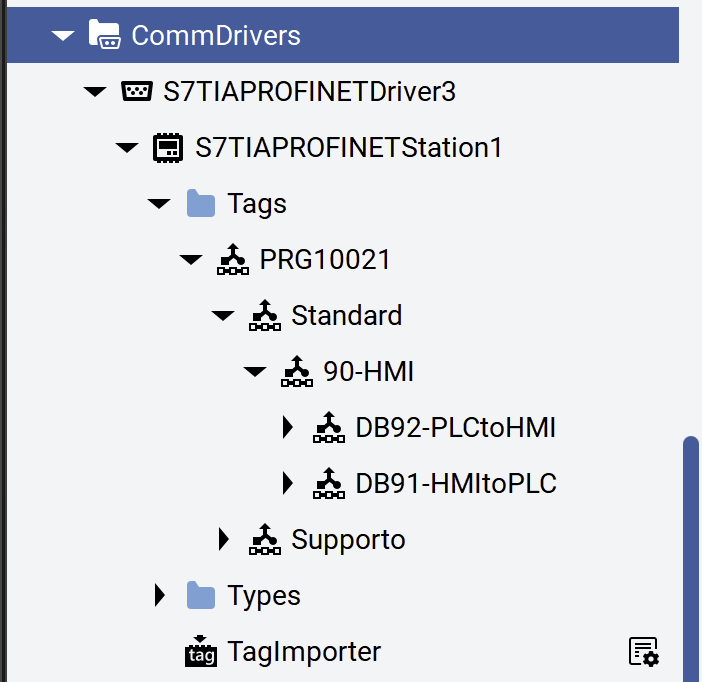
\includegraphics[width=0.4\linewidth]{Immagini/ImportTag.png}
    \caption{Illustrazione Tag importati}
    \label{fig:ImportTag.png}
\end{figure}

\section{Configurazione variabili}
Per quanto riguarda la gestione dei tag importati in precedenza, ci sono due strade da poter percorrere: lavorare direttamente sui tag importati con il rischio di avere accessi indesiderati e difficoltà nella manutenzione del sistema; oppure definire un livello di astrazione che separi i tag PLC dalle funzionalità dell'HMI. Per ovviare al problema della prima strada, adottiamo l'approccio che prevede sin da subito la creazione di variabili di modello in FT Optix™, per poi renderle intermediarie tra i tag del PLC e le funzionalità di FT Optix™. Questo approccio permette di rendere molto più sicuro l'utilizzo dell'HMI non avendo accessi diretti ai tag, e favorisce un maggior controllo dello SCADA. In secondo luogo si utilizza uno script per creare associazioni bidirezionali (\textit{dynamic links})\textsuperscript{\cite{factorytalk_setdynamiclink}} tra le variabili appena create e i tag importati dal PLC. Partiamo con il creare le variabili di modello, per cui è sufficiente creare all'interno della sezione Project view sotto la voce \verb|Model,| una cartella \verb|Drivers| in cui si definiscono tutte le variabili. Ovviamente le variabili devono essere configurate con nomi significativi per facilitare l'identificazione e l'uso. Una volta definite le variabili di modello, si passa alla parte di associazione, grazie ad un nuovo script di tipo \verb|Design-time NetLogic| in cui viene creata una funzione che comprenda la seguente struttura:
\begin{itemize}
    \item \textbf{Lista variabili di modello}: le variabili di modello sono ottenute tramite il metodo \verb|GetVariable|, specificando il path all'interno della struttura di progetto. Per ottenere il path eseguiamo gli stessi passaggi illustrati nei capitoli precedenti.
    \item \textbf{Lista dei tag PLC}: analogamente, i tag del PLC sono identificati con il loro path sotto la sezione \verb|CommDrivers|.
    \item \textbf{Creazione dynamic link}: l'associazione tra le variabili di modello e i tag del PLC avviene grazie al metodo \verb|SetDynamicLink| fornito da FT Optix™, configurato con la modalità \verb|ReadWrite| nel caso di lettura e scrittura su variabile, \verb|Read| per la lettura e \verb|Write| per la sola scrittura.
\end{itemize}
\begin{minted}[bgcolor=bgcolor, 
               linenos=true, 
               numbersep=8pt, 
               fontfamily=tt, 
               fontsize=\tiny, 
               breaklines=true, 
               breakanywhere=true]{csharp}
...

public class AssociazioneVarModelloAPLC : BaseNetLogic
{
    [ExportMethod]
    public void Method1()
    {
        /*------------------------------------------------
          variabili di modello 
        */
        
        //DB91
        var modello000 = Project.Current.GetVariable("Model/Drivers/DB91/DB91_CambioProduzione");
        ... // la lista prosegue con tutte le variabili di modello

        /*------------------------------------------------
          variabili di PLC
        */

        // DB91
        var varPLC000 = Project.Current.GetVariable("CommDrivers/S7TIAPROFINETDriver3/S7TIAPROFINETStation1/Tags/PRG10021/Standard/90-HMI/DB91-HMItoPLC/CambioProduzione");
        ... // la lista prosegue con tutte le variabili di PLC

        /*------------------------------------------------
          dynamicLink per Optix
        */
        modello000.SetDynamicLink(varPLC000, DynamicLinkMode.ReadWrite);
        ... // la lista prosegue con tutti i dynamicLink tra la prima e seconda lista
        
        }
}
\end{minted}
Questa modalità ha molteplici vantaggi. Prima di tutto, la sicurezza è migliorata: l'astrazione evita che l'HMI interagisca direttamente con i tag del PLC e permette di impostare la modalità in lettura e/o scrittura, che riduce significativamente il rischio di accesso non autorizzato. Inoltre, la manutenzione viene semplificata: la separazione tra modello e tag facilita eventuali modifiche future al sistema ed un eventuale reimpiego dell'HMI. Infine, la scalabilità: l’utilizzo di uno script per la configurazione consente di gestire facilmente un numero elevato di variabili e tag direttamente in un'unica funzione. Nonostante i numerosi vantaggi offerti da questo approccio, è importante evidenziare alcune criticità operative legate a sistemi complessi con migliaia di variabili. Più nello specifico, nei sistemi con elevato numero di variabili, il processo di messa a punto diventa un'operazione altamente dispendiosa in termini di tempo. Ciò accade perché ogni variabile di modello viene associata al corrispondente tag PLC tramite script. Una soluzione plausibile per sistemi avanzati potrebbe essere di automatizzare lo script di configurazione tramite il mapping delle variabili.

\subsection{Gestione FTP Robot, FTP Pressa e passi 50, 55 e 60}
Nei \verb|case 50, 55 e 60| citati in precedenza, vengono gestiti tutti i caricamenti dei programmi, sia della pressa piegatrice, sia del robot dell'impianto. Per richiesta, è stato scelto sin dall'inizio di gestire entrambi i programmi lato interfaccia, con la seguente lettura dei dati tramite macchina a stati. Partendo dalla progettazione HMI, entrambi i pannelli sono stati inseriti nella sezione impostazioni, con accesso riservato solo agli utenti con autorizzazione appropriata, come in figura \ref{fig:FTP.png}.
\begin{figure} [ht]
    \centering
    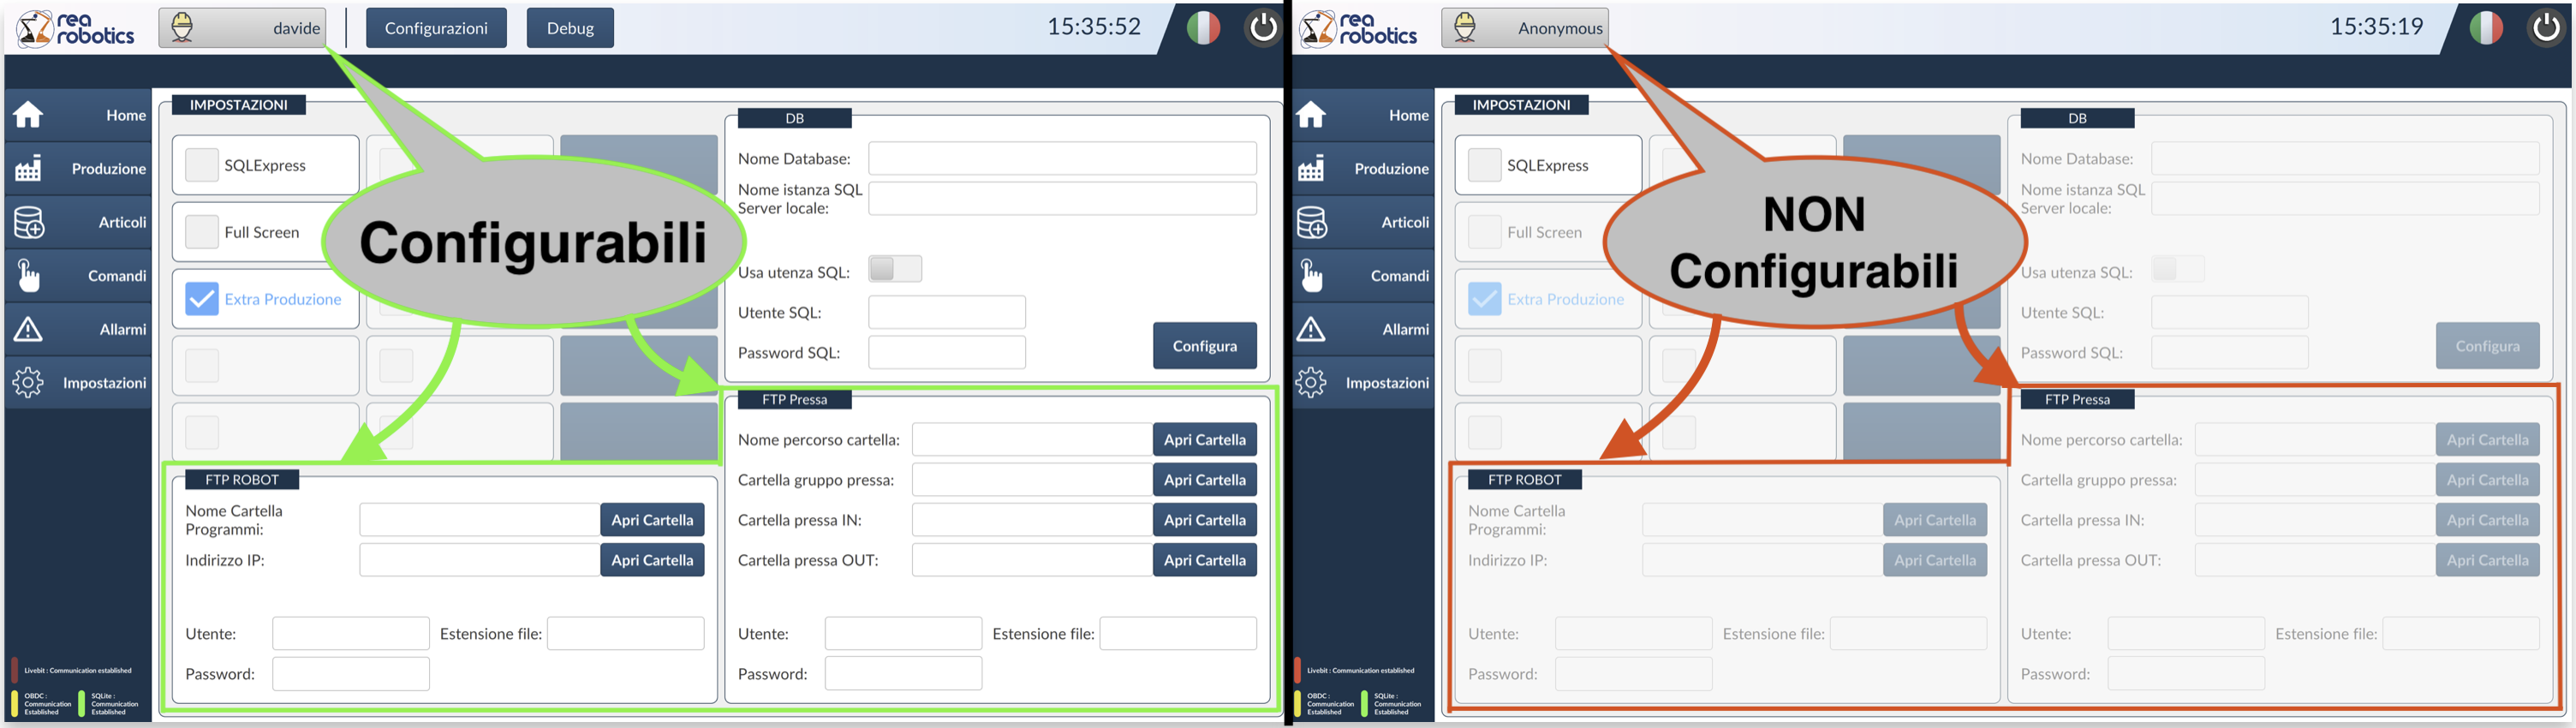
\includegraphics[width=\linewidth]{Immagini/FTP.png}
    \caption{Illustrazioni Gestione FTP Robot ed FTP Pressa}
    \label{fig:FTP.png}
\end{figure}

Entrando nello specifico, in questa sezione sono stati inseriti 2 pannelli che rispettassero i seguenti requisiti:
\begin{enumerate}
    \item \textbf{FTP Robot:} in cui è permesso selezionare il nome della cartella contenente i programmi robot, con estensione ed altri parametri specifici dell'impianto.
    \item \textbf{FTP Pressa:} richiede informazioni più dettagliate, tra cui le cartelle di input ed output del programma, oltre al nome specifico per la pressa e le credenziali di rete per un'eventuale gestione tramite FTP.
\end{enumerate}
Queste due sezioni sono fondamentali per poter riuscire a far comprendere all'impianto che tipo di istruzioni debba eseguire la macchina (robot e/o pressa) durante il caricamento di un ordine di produzione. I file contenenti le istruzioni del robot e quelli per la pressa vengono prodotti rispettivamente da chi si occupa della gestione robot e della gestione pressa. Per quanto riguarda, invece, la lettura tramite macchina stati, i passi da analizzare sono il 50, 55 e 60:
\begin{itemize}
    \item \verb|case 50|: in questo passo, il sistema si trova in attesa della richiesta da parte del PLC del caricamento del programma. Una volta ricevuta, in caso affermativo il sistema passa al passo 55; in caso di KO invece il passo viene impostato a 180.
    \item \verb|case 55|: il sistema esegue una serie di operazioni in cui vengono lanciate le funzioni di gestione programma, con annesso controllo dell'esistenza del file nel percorso indicato, copia del file dalla sorgente alla destinazione e verifica della consistenza del file copiato. Inoltre, ogni funzione ha una gestione degli errori con popup adeguati, restituendo valori in base all'esito (questa parte è presente in \verb|script_maincycle.cs|). Se tutto avviene in modo corretto, si passa al passo 60.
    \item \verb|case 60|: seconda ed ultima fase di attesa da parte dell'HMI nei confronti del PLC. Più nello specifico, l'HMI verifica che la variabile di richiesta caricamento programma desiderato sia resettata dal PLC, ed in base al risultato di questa verifica, il sistema decide quali saranno i prossimi passi da eseguire.
\end{itemize}
Quello che abbiamo analizzato in questo capitolo è la minima parte di tutto il lavoro che compone la gestione dei robot e di altri vari componenti presenti in un impianto; nel nostro caso la gestione era di due sole macchine con istruzioni ben definite. In contesti industriali più complessi, dove sono coinvolti numerosi apparati e macchine, la gestione può risultare molto più articolata e richiede soluzioni più sofisticate per garantire scalabilità, sincronizzazione e gestione di malfunzionamenti.

\begin{figure} [ht]
    \centering
    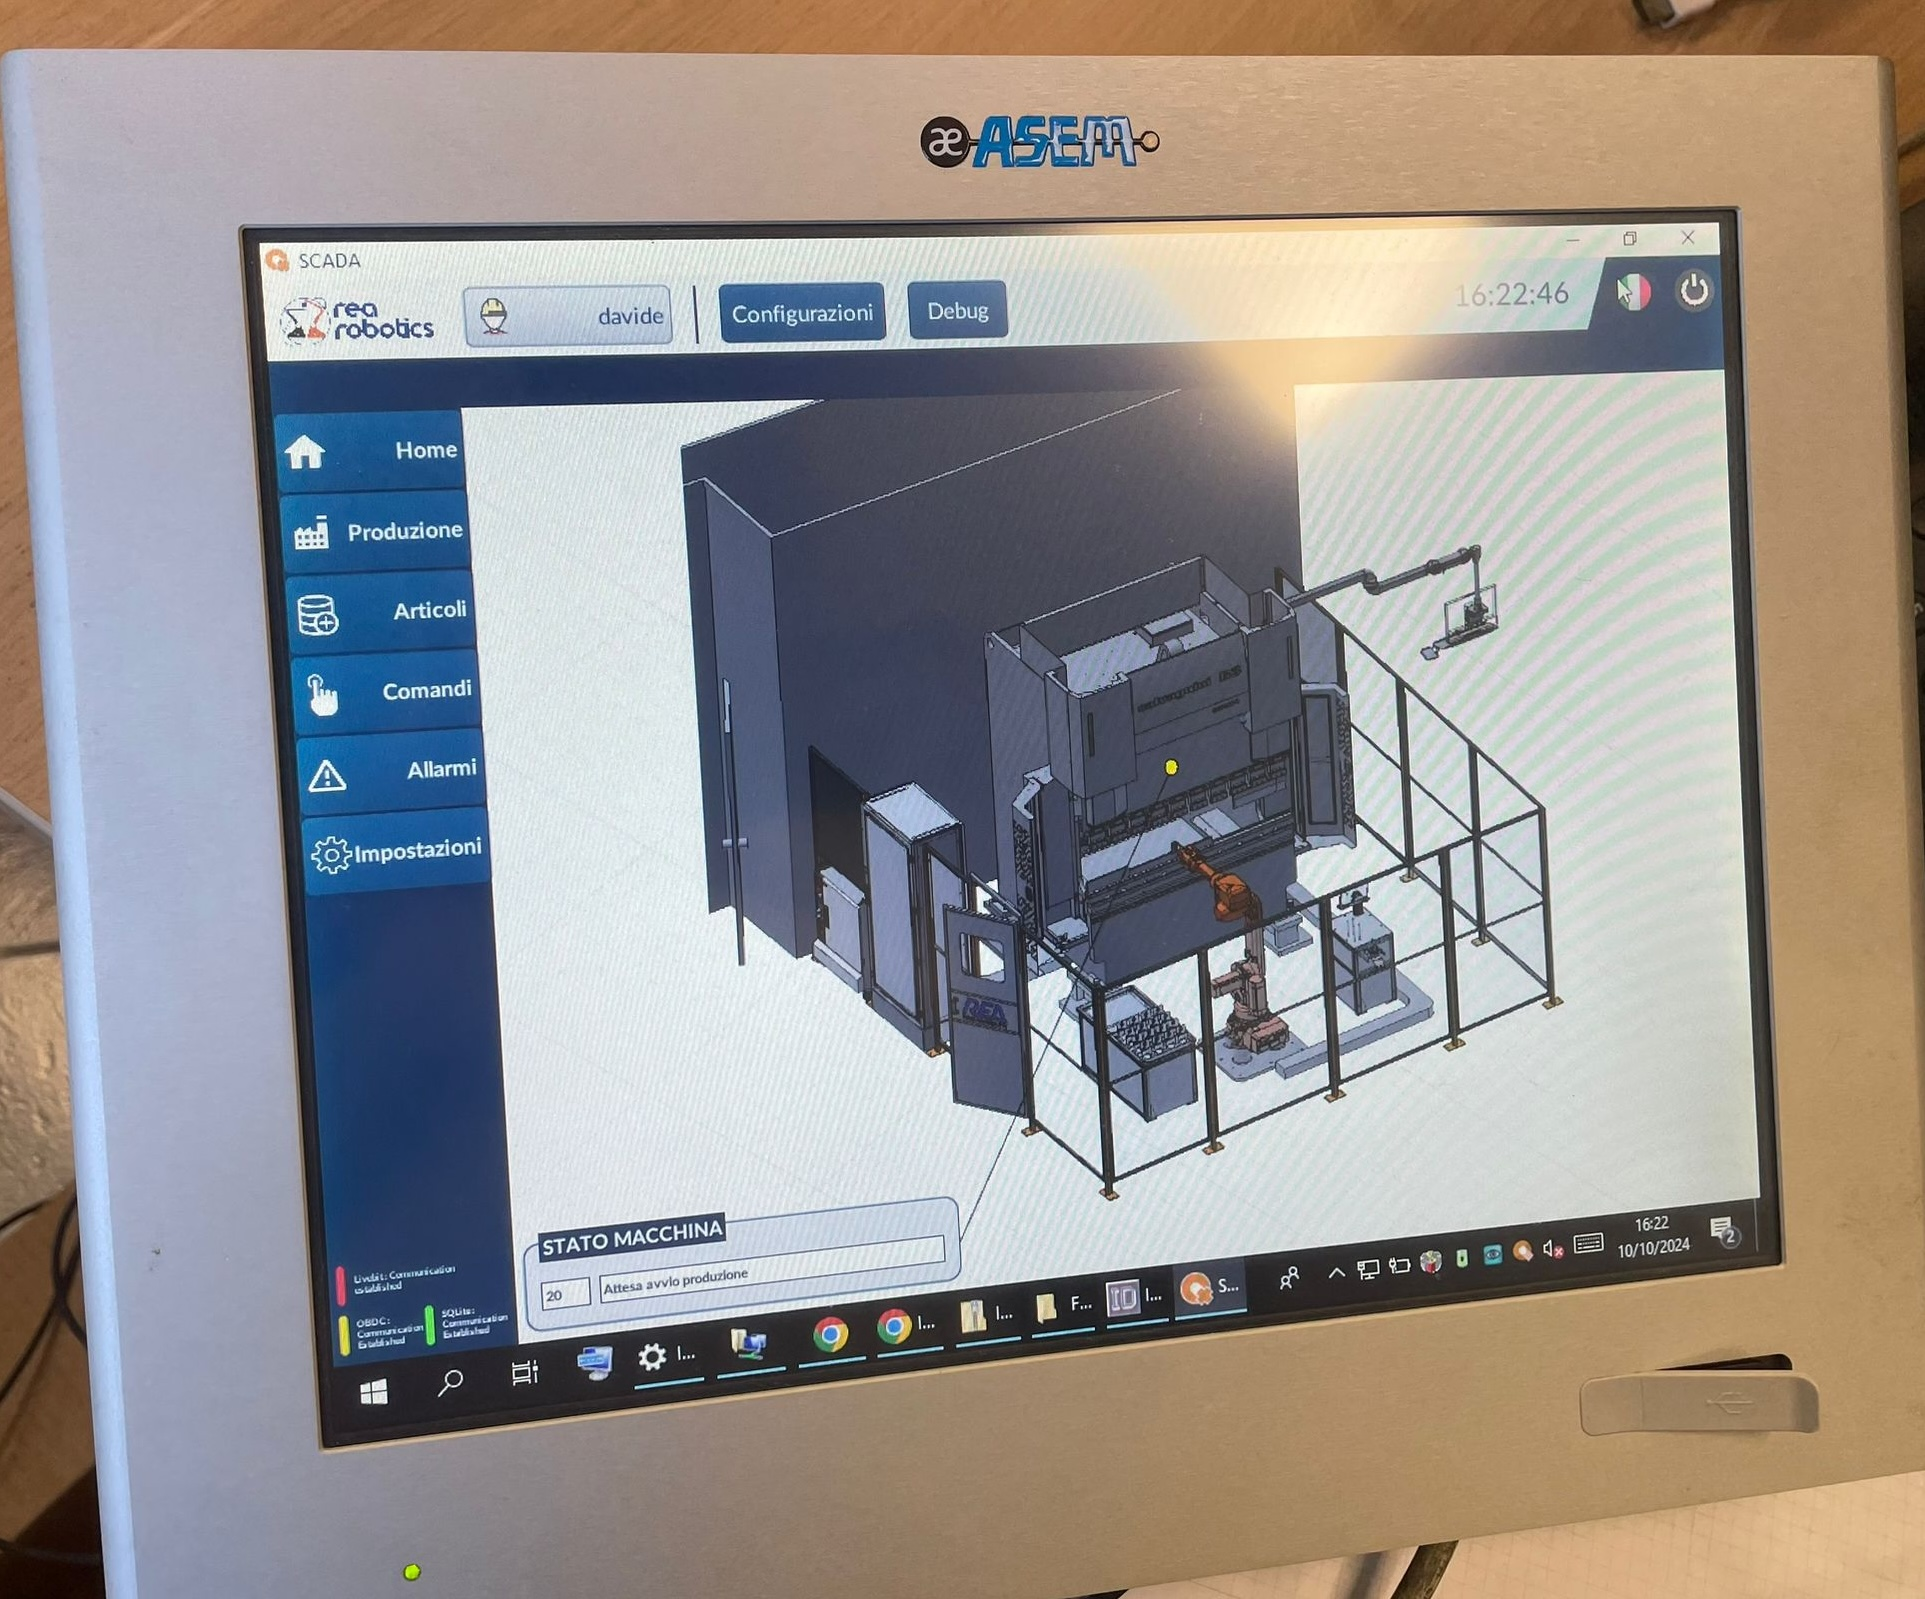
\includegraphics[width=0.7\linewidth]{Immagini/PannelloASEM.jpg}
    \caption{Prova messa in funzione dello SCADA su pannello prova ASEM}
    \label{fig:PannelloASEM.jpg}
\end{figure}
    \chapter{Conclusioni}

Il lavoro svolto per questa tesi ha avuto come obiettivo principale lo sviluppo di una soluzione SCADA integrata per la gestione di sistemi industriali, con focus sulle tecnologie utilizzate in REA Robotics. Nello specifico, la finalità è stata di implementare una piattaforma in grado di gestire in modo efficiente e sicuro il flusso di dati tra HMI e PLC, non solo permettendo di rispondere con successo alla task iniziale fornita dall'azienda, ma anche garantendo funzionalità operativa, sicurezza ed affidabilità del sistema. Il progetto ha visto come cardini l'utilizzo di strumenti e software come FT Optix™, C\#, SSMS e SQLite, per permettere la realizzazione di un'interfaccia che semplifica il monitoraggio e controllo dei macchinari. Nonostante sia stata raggiunta la task richiesta, sono emerse alcune criticità che meritano attenzione. Una delle principali sfide è stata la gestione separata dei due database, che ha comportato maggiore complessità nella progettazione da un lato e nella manutenzione futura dall'altro. Sarebbe auspicabile in futuro unificare la parte di database in un'unica implementazione generica che permetta una gestione più scorrevole, al fine di semplificare la mole di dati e codice presente e ridurre il rischio di incoerenze. Un'altra criticità riscontrata riguarda l'utilizzo dei recipe schema. La rigida dipendenza dalle regole imposte dal sistema di gestione di questi ultimi ha limitato la flessibilità del progetto, rendendo difficile adattare il sistema a future modifiche o implementazioni per altri impianti. In tal senso, una possibile evoluzione futura potrebbe prevedere il refactoring di alcuni script di codice per permettere la gestione dei dati più modulare e indipendente dalle regole imposte dai recipe schema, garantendo maggiore personalizzazione per i clienti. Guardando al futuro, sono diverse le opportunità di miglioramento e sviluppo. Per esempio, l'uso di C\# per ottimizzare la lettura delle variabili dei PLC consentirebbe un aggiornamento in tempo reale dei dati, una maggiore reattività del sistema alle modifiche e soprattutto meno tempo da dedicare lato programmazione, grazie a una gestione intelligente dei dynamic link attraverso una lettura diretta delle variabili. Inoltre, l'integrazione di Intelligenza Artificiale per l'analisi dei dati e per la progettazione dei pannelli potrebbe aprire nuovi scenari, consentendo una gestione ancora più efficiente dal lato software.

In conclusione, il progetto ha raggiunto gli obiettivi prestabiliti, complice un nuovo approccio nel contesto industriale di REA Robotics. Tuttavia, le criticità emerse durante lo sviluppo offrono sia spunti di riflessione, sia indicazioni per futuri miglioramenti. L'implementazione di soluzioni più moderne e flessibili, una gestione più modulare dei dati e l'introduzione di nuove tecnologie rappresentano sfide importanti per il futuro, con l'obiettivo di rendere questa tipologia di sistemi SCADA ancora più performante, sicura e adattabile alle esigenze in continua evoluzione dell'industria 4.0.
    \cleardoublepage

    \printbibliography[heading=bibintoc, title={Bibliografia e Sitografia}]
\end{document}
